\ifnum\aluno=1
\renewcommand\chapterillustration{./abertura-funcao-quadratica}
\else
\renewcommand\chapterillustration{abertura-funcao-quadratica-professor}
\fi
\renewcommand\chapterwhat{Função quadrática com enfoque na representação algébrica ou gráfica, entendendo suas aplicações tanto em problemas de otimização quanto na utilização das propriedades da curva (parábola) nas diversas áreas do conhecimento.}
\renewcommand\chapterbecause{As funções quadráticas apresentam-se especialmente em problemas que chamamos de otimização, onde o objetivo é determinar em que condições uma grandeza assume valores máximo ou mínimo, como por exemplo, o lucro máximo de uma empresa, área máxima de uma região plana, o preço mínimo de um determinado produto sujeito a condições específicas e assim por diante. Além disso, servem de modelo para os estudos físicos do movimento onde há aceleração constante, e possui aplicação em diversas áreas como: engenharia, economia, administração, ciência da computação etc.}
\chapter{Função Quadrática}
\label{\detokenize{AF209::doc}}\label{\detokenize{AF209:funcao-quadratica}}

\ifdefined\funcoeschap
\else
\label{chap-funcoes}
\label{numeros-triangulares-funcoes}
\fi
\def\estchapdois{}

\mbox{}\thispagestyle{empty}\clearpage

\thispagestyle{empty}

\begin{center}
Projeto: LIVRO ABERTO DE MATEMÁTICA

\noindent \begin{tabular}{lcccr}

\includegraphics[scale=.15]{impa}& \quad\quad& 
\includegraphics[width=3cm]{logo} & \quad\quad& 
\includegraphics[scale=.24]{obmep} 
\end{tabular}
\end{center}

\vspace*{.3cm}

Cadastre-se como colaborador no site do projeto: \url{umlivroaberto.org}

Versão digital do capítulo:

\url{https://www.umlivroaberto.org/BookCloud/Volume_1/master/view/AF209.html}


\begin{tabular}{p{.15\textwidth}p{.7\textwidth}}
Título: & Função Quadrática\\
\\
Ano/ Versão: & 2020 / versão 1.1 de \today\\
\\
Editora & Instituto Nacional de Matem\'atica Pura e Aplicada (IMPA-OS)\\
\\
Realização:& Olimp\'iada Brasileira de Matem\'atica das Escolas P\'ublicas (OBMEP)\\
\\
Produção:& Associação Livro Aberto\\
\\
Coordenação:& Fabio Simas, \\
			& Augusto Teixeira (livroaberto@impa.br)\\
\\
  Autores: & Luiz Amorim (Colégio Pedro II),\\
           & Bruno Vianna (Colégio Pedro II).\\

\\
Revisão &  Cydara Ripoll,  \\
        &  Letícia Rangel \\
\\
Design: & Andreza Moreira (Tangentes Design) \\
\\
  Ilustrações: & --- \\ 
\\
Gráficos: & Beatriz Cabral e Tarso Caldas (Licenciandos da UNIRIO)\\
\\
  Capa: & Foto de Ashkan Forouzani, no Unsplash\\
  		& https://unsplash.com/photos/J4idEoFc8k8 \\

\end{tabular}
\vspace{.5cm}


\begin{figure}[b]
\begin{minipage}[l]{5cm}
\centering

{\large Licença:}

  
\includegraphics[width=3.5cm]{cc-by-sa1}
\end{minipage}\hfill
\begin{minipage}[c]{5cm}
\centering
{\large Desenvolvido por}


\includegraphics[width=2.5cm]{logo-associacao.jpg}
\end{minipage}
\begin{minipage}[r]{5cm}
\centering

{\large Patrocínio:}
  \vspace{1em}
  
\includegraphics[width=3.5cm]{itau}
\end{minipage}
\end{figure}

\mainmatter

\begin{apresentacao}{Introdução}
Neste capítulo contemplam-se as seguintes habilidades da segunda versão da Base Nacional Comum Curricular (BNCC):

\begin{habilities}{EM12MT09}
Reconhecer função quadrática e suas representações algébrica e gráfica, compreendendo o modelo de variação determinando domínio, imagem, máximo e mínimo, e utilizar essas noções e representações para resolver problemas como os de movimento uniformemente variado.
\end{habilities}

\paragraph{Pré-requisitos}
\begin{habilities}{EF08MT15}
Resolver e elaborar problemas que possam ser representados por equações polinomiais de 2\super{o} grau do tipo $ax^2=b$.

\tcbsubtitle{EF09MT18}
Compreender os processos de fatoração de expressões algébricas, a partir de suas relações com os produtos notáveis, para resolver e elaborar problemas que possam ser representados por equações polinomiais de 2\super{o} grau.
\end{habilities}

\section{Objetivos gerais}

\begin{itemize}
\item {} 
Motivar o conceito de função quadrática por meio do movimento uniformemente variado (M.U.V.).

\item {} 
Explorar de modo intuitivo, as principais propriedades da função quadrática, com ênfase no seu gráfico.

\item {} 
Explorar o conceito de otimização, por meio da forma canônica, em situações que possam ser modeladas por funções quadráticas.

\item {} 
Inferir que o gráfico de toda função quadrática é uma parábola e que pode ser obtido por translações da função real \(f\) definida por \(f(x)=ax^2\) (\(a \in \mathbb{R}\)), definindo formalmente suas formas polinomiais e canônicas.

\item {} 
Apresentar situações modeladas por funções quadráticas de domínio discreto.

\item {} 
Determinar os zeros de uma função quadrática bem como seus intervalos de crescimento e decrescimento, tanto por meio de sua expressão algébrica como de sua representação gráfica.

\item {} 
Reconhecer o eixo de simetria do gráfico de uma função quadrática.

\item {} 
Determinar a lei de formação de uma função quadrática apresentando seu gráfico.

\end{itemize}

Prezado colega, neste capítulo buscamos contemplar os conceitos, propriedades, definições e aplicações relacionadas ao estudo das funções quadráticas de modo gradativo e por meio de atividades que guiarão os alunos para os objetivos deste capítulo, mencionados anteriormente. Optamos, por influência da habilidade do BNCC, introduzir os conceitos mais básicos por uma atividade que estuda o movimento de queda livre de um objeto. De posse desses conceitos básicos, partimos para a segunda atividade que tem como objetivo geral de familiarizar os alunos com o gráfico de uma função real \(f\) definida por \(f(x)=x^2\), chamando a atenção para suas caracteríticas e propriedades.

Nas atividades seguintes exploramos problemas de otimização. Optamos por abordar esse assunto utilizando a forma canônica da função quadrática, pois é fato que a mesma já exibe claramente as coordenadas do vértice da parábola, facilitando assim a descoberta desse valor (máximo ou mínimo). Além disso, a forma canônica permite, de modo simples, apresentar ao aluno que todos os gráficos das funções quadráticas podem ser obtidos por translações do gráfico da função real \(f\) definida por \(f(x)=ax^2\) apresentado nas atividades iniciais do capítulo.

Para concluir o capítulo, aplicamos os conhecimentos adquiridos em problemas nos quais a modelagem faz uso de uma aproximação por parábolas e, nesses casos, o estudante precisa determinar a lei de formação da função quadrática por meio de informações gráficas inicialmente apresentadas.

Por fim, na seção “Você sabia?”, abordamos dois assuntos de extrema importância: A utilização prática da parábola que vem como consequência da sua propriedade refletora, e desfazemos alguns equívocos frequentes que ocorrem ao se admitir que algumas curvas ou situações podem ser modeladas por funções quadráticas.

\subsection{Dificuldades típicas dos alunos (distratores)}

\begin{itemize}

\item {} 
Os alunos conhecem a denominação correta do gráfico apresentado pela função quadrática, porém, não conseguem distingui-lo de outros gráficos curvilíneos. \citep{alexandre2009}

Distrator trabalhado na atividade \hyperref[\detokenize{AF209-2:ativ-funcao-quadratica-investigando-x-a-2}]{\textit{Em busca de padrões em \(f(x)=x^2\)}} e em \hyperref[\detokenize{AF209-11:sub-funcao-quadratica-voce-sabia-catenaria}]{Será que é parábola?}.

\item {} 
Os alunos sabem, conceitualmente, a relação existente entre os eixos das abscissas e ordenadas na função quadrática, mas não possuem habilidades de diferenciá-los durante o processo da resolução de uma questão contextualizada envolvendo função quadrática. \citep{alexandre2009}

Distrator trabalhado em: \hyperref[\detokenize{AF209-0:ativ-funcao-quadratica-lancamento-vertical-em-dubai}]{\textit{Lançando objetos das nuvens em Dubai}}, \hyperref[\detokenize{AF209-3:sub-ativ-funcao-quadratica-perimetro-fixo}]{\textit{Perímetro fixo}}, \hyperref[\detokenize{AF209-7:ativ-funcao-quadratica-aumento-passagem}]{\textit{Aumento da passagem}}, \hyperref[\detokenize{AF209-9:sec-funcao-quadratica-obtendo-lei-do-grafico}]{Explorando: determinando a função quadrática através do gráfico}.

\item {} 
Os alunos compreendem a qual eixo está relacionado, genericamente, o domínio e a imagem, porém não conseguem particularizá-lo à função quadrática. \citep{alexandre2009}

Distrator trabalhado em: \hyperref[\detokenize{AF209-0:ativ-funcao-quadratica-lancamento-vertical-em-dubai}]{\textit{Lançando objetos das nuvens em Dubai}}, \hyperref[\detokenize{AF209-3:sub-ativ-funcao-quadratica-perimetro-fixo}]{\textit{Perímetro fixo}}, \hyperref[\detokenize{AF209-7:ativ-funcao-quadratica-aumento-passagem}]{\textit{Aumento da passagem}}, \hyperref[\detokenize{AF209-9:sec-funcao-quadratica-obtendo-lei-do-grafico}]{Explorando: determinando a função quadrática através do gráfico}.

\item {} 
Há uma grande dificuldade em utilizar processos simples de fatoração para representar uma função quadrática em sua forma fatorada, consequentemente na busca dos zeros da função. \citep{parent2015}

Distrator trabalhado em: \hyperref[\detokenize{AF209-3:sub-ativ-funcao-quadratica-perimetro-fixo}]{\textit{Perímetro fixo}}, \hyperref[\detokenize{AF209-7:ativ-funcao-quadratica-aumento-passagem}]{\textit{Aumento da passagem}}, \hyperref[\detokenize{AF209-8:sec-funcao-quadratica-org-ideias-intersecoes-com-eixos}]{Organizando as ideias: interseção com os eixos coordenados}, \hyperref[\detokenize{AF209-9:sec-funcao-quadratica-obtendo-lei-do-grafico}]{Explorando: determinando a função quadrática através do gráfico}.

\item {} 
“{[}…{]}os estudantes ficam confusos quando as equações quadráticas são apresentadas de maneira não usual pois não são exatamente como estes estão acostumados a vê-las. Por o exemplo, ao apresentar \(x^2 + 3x + 1 = x + 4\) que não está em forma padrão, vários alunos apresentam dificuldades quando solicitados a realizarem várias tarefas. \citep{kotsopoulos2007}

Distrator trabalhado em: \hyperref[\detokenize{AF209-3:sec-funcao-quadratica-org-ideias-quad-max-min-na-quadratica}]{Organizando as ideias: máximos ou mínimos} , \hyperref[\detokenize{AF209-3:sub-ativ-funcao-quadratica-perimetro-fixo}]{\textit{Perímetro fixo}}, \hyperref[\detokenize{AF209-7:ativ-funcao-quadratica-aumento-passagem}]{\textit{Aumento da passagem}}.

\item {} 
Ao fazer alusão com a função afim alguns alunos acreditam equivocadamente que o coeficiente “a” da forma polinomial ou canônica representa a taxa de variação da função ou a “inclinação” de uma função quadrática. \citep{parent2015}

Distrator trabalhado em: \hyperref[\detokenize{AF209-3:sec-funcao-quadratica-org-ideias-quad-max-min-na-quadratica}]{Organizando as ideias: máximos ou mínimos}, \hyperref[\detokenize{AF209-5:sec-funcao-quadratica-parametros-grafico}]{Explorando: os parâmetros da forma canônica e o gráfico da função quadrática}.

\item {} 
Alguns alunos não associam a ideia de máximo ao \(a<0\) e ao mínimo ao \(a>0\), associam apenas ao valor numérico da expressão \(\frac{-\Delta}{4a}\), sem ao menos se preocupar se o domínio é um intervalo e se a ordenada do vértice está contida na imagem.

Distrator trabalhado em: \hyperref[\detokenize{AF209-3:sec-funcao-quadratica-org-ideias-quad-max-min-na-quadratica}]{Organizando as ideias: máximos ou mínimos}.

\item {} 
Há uma grande tendência dos alunos associarem a imagem da função quadrática ao gráfico da parábola e não a um conjunto de valores reais do eixo das ordenadas.

Distrator trabalhado em: \hyperref[\detokenize{AF209-0:ativ-funcao-quadratica-lancamento-vertical-em-dubai}]{\textit{Lançando objetos das nuvens em Dubai}}, \hyperref[\detokenize{AF209-2:sec-funcao-quadratica-org-ideias-em-x-a-2}]{Organizando as ideias: características da função real}, \hyperref[\detokenize{AF209-3:sub-ativ-funcao-quadratica-perimetro-fixo}]{\textit{Perímetro fixo}}, \hyperref[\detokenize{AF209-7:ativ-funcao-quadratica-aumento-passagem}]{\textit{Aumento da passagem}}.

\end{itemize}
\end{apresentacao}

\def\currentcolor{session1}
\begin{objectives}{Lançando objetos das nuvens em Dubai}
{
\begin{itemize}
\item Reconhecer que a relação matemática entre a distância percorrida por um objeto em queda livre e o tempo de queda não pode ser modelada por uma função afim.
\item Relacionar o movimento de queda livre de um objeto a existência de uma aceleração na velocidade de queda.
\item Inferir que o tempo é uma grandeza contínua, mesmo sendo finito o número de dados coletados.
\item Reconhecer que o movimento pode ser descrito por uma curva e não por um conjunto de pontos desconectos.
\end{itemize}
}{1}{1}
\end{objectives}
\begin{sugestions}{Lançando objetos das nuvens em Dubai}
{
\begin{itemize}
\item Sugerimos resolver a atividade anteriormente para definir o tempo necessário de sua aplicação.
\item Orientamos que seja feito um acompanhamento por parte do professor, durante a confecção da tabela apresentada no item a, com a finalidade de ter a certeza que os estudantes estejam compreendendo o significado dos valores gerados por ela.
\item Caso seja necessário, reforce as principais caracteríticas da função afim, como por exemplo: a sua taxa de variação constante.
\item No item \titem{d}, recomendamos que o professor chame a atenção dos estudantes para o fato de que, o gráfico seja apenas um conjunto de sete pontos, partindo da origem, e não uma curva contínua.
\item Para o item e, orientamos que o professor enfatize aos alunos que o registro fotográfico foi feito em intervalos de $1$ s, mas que o fenômeno continuou mesmo sem os registros.
\end{itemize}
}{1}{1}
\end{sugestions}
\clearmargin
\begin{answer}{Lançando objetos das nuvens em Dubai}
{
\begin{enumerate}
\item $d_0=0\text{ m}; d_1=5\text{ m}; d_2=20\text{ m}; d_3=45\text{ m}; d_4=80\text{ m}; d_5=125\text{ m}; d_6=180\text{ m}$.
\item Não. Para verificar, basta calcular a razão entre a variação das distâncias em dois intervalos distintos de um segundo, por exemplo: $\frac{5−0}{1−0}=5\neq\frac{20−5}{2−1}=15$, pois a função afim é caracterizada por uma variação constante.
\item Não, pois a taxa de variação não é constante.
\end{enumerate}
}{1}
\end{answer}
\clearmargin
\begin{answer}{Lançando objetos das nuvens em Dubai}
{
\begin{enumerate}\setcounter{enumi}{3}
\item \adjustbox{valign=t}
{
\begin{tikzpicture}[yscale=.8, xscale=1.2, scale=.75]
\tikzstyle{ponto}=[circle, minimum size=5pt, inner sep=0, draw=black, fill=black, shift only, label={}]
\draw [help lines, secundario!10, step=0.2] (0,0) grid (7,11);
\draw [help lines, secundario!40] (0,0) grid (7,11);
\draw [very thick, <->] (7.1,0) -- (0,0) -- (0, 11.1);
\node [below ] at (6.3,-0.5) {Tempo (s)};
\node [left] at (-0.5, 10.7) {Dist\^ancia (m)};
\node [below] at (0,0) {0};
\node [below] at (1,0) {1};
\node [below] at (2,0) {2};
\node [below] at (3,0) {3};
\node [below] at (4,0) {4};
\node [below] at (5,0) {5};
\node [below] at (6,0) {6};
\node [left] at (0,1) {20};
\node [left] at (0,2) {40};
\node [left] at (0,3) {60};
\node [left] at (0,4) {80};
\node [left] at (0,5) {100};
\node [left] at (0,6) {120};
\node [left] at (0,7) {140};
\node [left] at (0,8) {160};
\node [left] at (0,9) {180};
\node [left] at (0,10) {200};
\node [ponto, color=primario] at (1,0.25) {};
\node [ponto, color=primario] at (2,1) {};
\node [ponto, color=primario] at (3,2.25) {};
\node [ponto, color=primario] at (4,4) {};
\node [ponto, color=primario] at (5,6.25) {};
\node [ponto, color=primario] at (6,9) {};
\end{tikzpicture}
}
\item Sim, pois o tempo é contínuo.
\item Curva
\item $d(t)=5t^2$
\end{enumerate}
}{1}
\end{answer}
\clearmargin
\begin{objectives}{Distância segura entre os carros}
{
\begin{itemize}
\item Relacionar a frenagem com a existência da desaceleração.
\item Registrar que mesmo o texto indicando uma proporcionalidade, que a relação entre as grandezas discutidas na atividade não é uma função afim.
\item Reforçar a ideia de que a função afim não modela a variação do deslocamento para movimentos acelerados.
\item Expressar matematicamente uma informação dada na forma de texto.
\item Perceber que a desaceleração é mais intensa no seco do que no molhado, desenvolvendo as noções intuitivas necessárias à compreensão dos movimentos uniformemente variados.
\end{itemize}
}{1}{2}
\end{objectives}
\begin{answer}{Distância segura entre os carros}
{
\begin{enumerate}
\item $80\div3{,}6=2009\approx22$. Assim, o carro se desloca aproximadamente $22$ m nesse segundo.
\item $57−22=35$ m.
\item $D=kv2$
\item $k=\frac{D}{v^2}\iff k=\frac{35}{80^2}\iff k=\frac{7}{1280}\implies k\approx0{,}0055$.
\item Não.
\item $a=25\text{ m}; b\approx45 \text{ m}; c=70 \text{ m}; f\approx28 \text{ m}; g=55 \text{ m}; h=83 \text{ m}.$ Os valores a serem preenchidos na faixa azul de pista molhada exigem uma outra relação de $D$ e $v$: $\frac{D}{v^2}=\frac{71}{80^2}\iff\frac{D}{v^2}=\frac{71}{6400}\implies D=0{,}01\cdot v^2$, aproximadamente. Assim, $d=81 \text{ m}; e=106 \text{ m}; i=100 \text{ m}; j=128 \text{ m}$.
\end{enumerate}
}{1}
\end{answer}

\explore{Movimentos com Velocidade Variável}
\label{\detokenize{AF209-0:sec-funcao-quadratica-movimento-com-velocidade-variavel-queda-vertical}}\label{\detokenize{AF209-0::doc}}\label{\detokenize{AF209-0:explorando-movimentos-com-velocidade-variavel}}\phantomsection\label{\detokenize{AF209-0:ativ-funcao-quadratica-lancamento-vertical-em-dubai}}

Vamos agora conhecer um {}novo tipo de função real: as \textbf{funções quadráticas}. Também conhecidas como funções polinomiais do segundo grau, ela aparece em diversas situações do cotidiano, especialmente em problemas que chamamos de otimização, onde o objetivo é determinar em que condições uma grandeza assume valores máximos ou mínimos, como por exemplo, o lucro máximo de uma empresa, área máxima de uma região plana, o preço mínimo de um determinado produto e assim por diante. Assim como nos outros capítulos do Livro Aberto, vamos apresentar conceitos, definições e propriedades por meio de atividades e aprofundar esses conhecimentos na seção “Organizando Ideias”. Esperamos que você desfrute, se aproprie e aplique esses conceitos que serão úteis em diversas áreas do conhecimento, não só nos estudos físicos do movimento, mas em áreas como da engenharia, economia, administração, ciência da computação etc.

\begin{task}{Lançando objetos das nuvens em Dubai}

No topo do hotel Burj Al Arab, em Dubai, encontra-se a quadra de tênis mais alta do mundo, com aproximadamente \(200\) metros de altura. Em 2005, os campeões Roger Federer e Andre Agassi disputaram uma partida de exibição. Considere que por um descuido, uma das bolinhas usadas nesse jogo caiu \(200\)m, verticalmente e em queda livre. Vamos aproveitar essa situação para investigar a matemática por trás desse fenômeno físico. A imagem a seguir traduz a situação no início da queda da bola.

\begin{figure}[H]
\centering
\capstart

\noindent\includegraphics[width=140bp]{{fig_1}.jpg}
\caption{Hotel e a bolinha de tênis (\textbf{credito da imagem aqui}).}\label{\detokenize{AF209-0:id125}}\end{figure}

Um observador registra com seu equipamento fotográfico a queda da bolinha, disparando fotos a cada intervalo de \(1\) segundo, até a mesma atingir o solo. Os registros fotográficos encontram-se agrupados e animados na simulação da queda, que pode ser visualizada no Geogebra: Bola de Tenis (\url{https://ggbm.at/hvnNHMY2})

A tabela a seguir descreve a altura da bolinha ao longo do tempo.

\begin{table}[H]
\centering
\begin{tabu} to \textwidth{|c|c|c|}
\hline
\thead
\(t\) & Tempo (s) & Altura (m) \\
\hline
\(t_0\) & \(0\) & \(200\) \\ 
\hline
\(t_1\) & \(1\) & \(195\) \\
\hline
\(t_2\) & \(2\) & \(180\) \\
\hline
\(t_3\) & \(3\) & \(155\) \\
\hline
\(t_4\) & \(4\) & \(120\) \\
\hline
\(t_5\) & \(5\) & \(75\) \\
\hline
\(t_6\) & \(6\) & \(20\) \\
\hline
\end{tabu}
\end{table}

\begin{enumerate}
\item {} 
Numa folha de papel ou similar, reproduza a tabela a seguir e preencha o que falta, informando a distância total percorrida pela bolinha na queda, a partir de \(t_0\).

\begin{table}[H]
\centering
\begin{tabu} to \textwidth{|c|l|}
\hline
\thead
Tempo de Queda & Distância percorrida pela bolinha \\
\hline
De \(t_0\) a \(t_0 = 0\)s & \(d_0 = 200 - 200 = 0\)m \\
\hline
De \(t_0\) a \(t_1  = 1\)s & \(d_1 = 200 - 195 = 5\)m \\
\hline
De \(t_0\) a \(t_2 = 2\)s & \(d_2 =\) \\
\hline
De \(t_0\) a \(t_3 = 3\)s & \(d_3 =\) \\
\hline
De \(t_0\) a \(t_4 = 4\)s & \(d_4 =\) \\
\hline
De \(t_0\) a \(t_5 = 5\)s & \(d_5 =\) \\
\hline
De \(t_0\) a \(t_6 = 6\)s & \(d_6 =\) \\
\hline
\end{tabu}
\end{table}


\item {} 
As distâncias percorridas pela bolinha ao longo do tempo de queda aumentam com a mesma taxa de variação?

\item {} 
É possível obter uma função afim que relaciona a distância percorrida \(d_n\) (em metros) com o tempo de queda \(t\) (em segundos)? Justifique.

\item {} 
Em uma folha de papel ou similar, copie o plano cartesiano abaixo e, em seguida, represente os pares ordenados \((t;d_n)\) em que \(t\) representa o tempo de queda em segundos e \(d_n\) a distância, em metros, percorrida pela bolinha na queda:



\begin{figure}[H]
\centering

\begin{tikzpicture}[yscale=.8, xscale=1.2]
Gráfico
\tikzstyle{ponto}=[circle, minimum size=5pt, inner sep=0, draw=black, fill=black, shift only, label={}]
\draw [help lines, secundario!10, step=0.2] (0,0) grid (7,11);
\draw [help lines, secundario!40] (0,0) grid (7,11);
\draw [very thick, <->] (7.1,0) -- (0,0) -- (0, 11.1);
\node [below ] at (6.3,-0.5) {Tempo (s)};
\node [left] at (-0.5, 10.7) {Distância (m)};
\node [below] at (0,0) {0};
\node [below] at (1,0) {1};
\node [below] at (2,0) {2};
\node [below] at (3,0) {3};
\node [below] at (4,0) {4};
\node [below] at (5,0) {5};
\node [below] at (6,0) {6};
\node [left] at (0,1) {20};
\node [left] at (0,2) {40};
\node [left] at (0,3) {60};
\node [left] at (0,4) {80};
\node [left] at (0,5) {100};
\node [left] at (0,6) {120};
\node [left] at (0,7) {140};
\node [left] at (0,8) {160};
\node [left] at (0,9) {180};
\node [left] at (0,10) {200};
\end{tikzpicture}
\end{figure}

\item {} 
O domínio da função que descreve a queda da bolinha ao longo do tempo é \(D = \{0 ; 1 ; 2 ; 3 ; 4 ; 5 ; 6 \}\). A mesma situação poderia ser descrita por uma função de domínio contínuo?

\item {} 
Neste caso, ao ligarmos todos os pontos do gráfico do item \(d\) teríamos um segmento de reta ou uma curva?

\item {} 
Dentre as alternativas a seguir, qual relação atende aos valores descritos no gráfico sendo \(d(t)\) a distância percorrida pela bolinha na queda (em metros) com o tempo de queda \(t\) (em segundos).

\(\Box \; d(t)= -t^2\)

\(\Box \; d(t)= 10t+10\)

\(\Box \; d(t)= 20t\)

\(\Box \; d(t)= 5t^2\)

\(\Box \; d(t)= 10t^2\)

\end{enumerate}
\end{task}

\phantomsection\label{\detokenize{AF209-0:ativ-funcao-quadratica-distancia-frenagem}}
\clearpage
\begin{task}{Distância segura entre os carros}

Uma noção importante sobre a direção defensiva trata do fato de que \textit{“Ao pisar no freio do veículo, ele não para instantaneamente. Entre o momento que o motorista observa um obstáculo à sua frente e decide acionar os freios até o instante que o carro realmente para, ele se desloca vários metros”} [\href{https://www.jcnet.com.br/noticias/geral/2013/02/367699-direcao-defensiva--saiba-como-a-velocidade-influi-na-frenagem-do-veiculo.html}{JCNET-2013}]. Esse fato gera a chamada \textbf{distância de frenagem}, que precisa ser conhecida, para a segurança de todo motorista.

Como essa distância depende de muitos fatores, logo que um veículo é lançado, revistas especializadas tratam de divulgar tabelas com as relações entre as velocidades e as distâncias de frenagem para estes veículos. A análise experimental e cuidadosa de qualquer uma dessas tabelas revela que a distância percorrida por um veículo após o acionamento dos freios é proporcional ao quadrado da sua velocidade [\href{http://rpm.org.br/cdrpm/12/5.htm}{Avila}].

No artigo [\href{https://www.jcnet.com.br/noticias/geral/2013/02/367699-direcao-defensiva--saiba-como-a-velocidade-influi-na-frenagem-do-veiculo.html}{JCNET-2013}] encontramos que um veículo a \(80\) Km/h, ao considerarmos os tempos de percepção, de reação e de parada, vai percorrer em média \(57\) metros em pista seca até parar totalmente, assim que o motorista observar o obstáculo e decidir frear.

\begin{enumerate}
\item {} 
Considere que o tempo de reação entre a percepção do obstáculo e a pisada no freio para um motorista seja de um segundo. Nesse tempo, quantos metros o seu carro se desloca, se inicialmente está a 80Km/h? {[}Se necessário, utilize que \(\upsilon\)Km/h = \(( \upsilon \div 3\text{,}6 )\)m/s{]}.

\item {} 
A distância de \(57\)m descrita no texto considera duas distância juntas: a que o móvel percorre no segundo anterior ao acionamento do freio, e a distância de frenagem. Sendo assim, quanto é somente a distância de frenagem desse móvel a \(80\)Km/h e que percorreu um total de \(57\)m antes de parar?

\item {} 
Sendo \(k\) uma constante de proporcionalidade, exiba uma relação algébrica entre a distância de frenagem e a velocidade do móvel antes do acionamento do freio, descrita no segundo parágrafo do texto.

\item {} 
Para os valores considerados no item \titem{b)}, qual o valor da constante de proporcionalidade \(k\)?

\item {} 
A relação algébrica obtida no item \titem{c)} é uma função afim?

Observe a figura a seguir. Ela exibe, na placa o número \(80\), referente a velocidade do carro antes de perceber o obstáculo e decidir freiar. Logo abaixo da placa há um Sol e uma nuvem de chuva. Isso é para indicar que a faixa vermelha revere-se a situação de frenagem com a pista seca, e a faixa azul a frenagem com pista molhada.

\begin{figure}[H]
\centering
\capstart

\noindent\includegraphics[width=400bp]{{frenagem1}.jpg}
\caption{Exemplo preenchido}\label{\detokenize{AF209-0:id127}}\end{figure}

\begin{figure}[H]
\centering
\capstart

\noindent\includegraphics[width=200bp]{{frenagem2}.jpg}
\caption{Significado das bandeiras nas figuras}\label{\detokenize{AF209-0:id128}}\end{figure}

\item {} 
Conforme o exemplo acima, determine todos os valores que estão faltando e que estão representados pelas letras de ‘a’ até ‘j’, observando a mudança nas placas de velocidade do carro antes de perceber o obstáculo e decidir freiar.

\end{enumerate}

\begin{figure}[H]
\centering

\noindent\includegraphics[width=400bp]{{frenagem3}.jpg}
\end{figure}
\end{task}


Na prática, para manter uma distância segura entre os carros e evitar o “engavetamento”, aconselha-se seguir a regra dos dois segundos:
\begin{itemize}
\item {} 
\textit{Observe a estrada à sua frente e escolha um ponto fixo de referência (à margem) como uma árvore, placa, poste, casa, etc.}

\item {} 
\textit{Quando o veículo que está à sua frente passar por este ponto, comece a contar pausadamente: cinqüenta e um, cinqüenta e dois. (mais ou menos dois segundos).}

\item {} 
\textit{Se o seu veículo passar pelo ponto de referência antes de contar (cinqüenta e um e cinqüenta e dois), deve aumentar a distância, diminuindo a velocidade, para ficar em segurança.}

\end{itemize}
% \begin{enumerate}
% \item {} 
% Quanto deu os resultados de cada uma dessas somas?

% \item {} 
% Com base nos itens ‘g’ e ‘h’, determine o resultado da soma de todos os números da primeira e da segunda linhas.

% \item {} 
% Lembrando do que você marcou no item ‘f’, determine o resultado obtido por \textit{Gauss}.

% \item {} 
% Você seria de capaz de refazer as etapas, porém desta vez encontrando uma expressão para o resultado da soma dos \(n\) primeiros números naturais? Ou seja, tente expressar em função de \(n\), o resultado de \(1+2+3+4+5+ \cdots +(n-3)+(n-2)+(n-1)+n\).

% \end{enumerate}

\arrange{Queda Vertical}
\label{\detokenize{AF209-1:sec-org-ideias-galileu-muv}}\label{\detokenize{AF209-1::doc}}\label{\detokenize{AF209-1:organizando-as-ideias-queda-vertical}}
\textbf{Aristóteles} (\(\star\) Estagira, \(384\) a.C. — \(\dagger\) Atenas, \(322\) a.C.) e \textbf{Galileu Galilei} \((\star 1564 , \dagger 1642)\) \textbf{no estudo da Queda Livre}

Aristóteles, discípulo de Platão e professor de Alexandre o Grande, foi um grande filósofo grego e seus estudos, nas mais diversas áreas, impactaram significativamente a história da humanidade.

Em sua época, a escola Platônica dominava a produção científica ocidental, e boa parte dela era influenciada pelo conceito de “natureza” de um objeto, onde se afirmava que todo objeto era composto da combinação dos quatro elementos: “terra, ar, água e fogo”. O estudo dos Movimentos de Aristóteles apresenta alguns equívocos que perpassaram por alguns séculos, devido a essas definições.

Aristóteles afirmava que havia dois tipos de movimentos: os naturais e os violentos. Os naturais, para ele, decorre diretamente da natureza do objeto e os violentos decorrem de  forças aplicadas a esses objetos, ou seja um movimento imposto.

No caso dos movimentos naturais, Aristóteles afirmava que cada objeto tem um lugar próprio na natureza e que esses se “esforçam” para retornar ao seu lugar de origem. Por exemplo um vaso de cerâmica, ao ser abandonado cai procurando seu lugar ao solo, já que em sua composição o elemento terra é o mais presente, e pelo mesmo motivo um sopro, ou “baforada” acaba se misturando com o ar.

Além disso, Aristóteles, afirmava que um objeto mais pesado (com maior massa) cai em direção ao solo, mais rapidamente que um objeto mais leve, ou seja, para ele, objetos ao serem lançados, caíam com rapidez proporcional ao seu peso. Suas afirmações sobre o movimento, pautaram o pensamento científico por mais de dois mil anos, sendo a base da ciência na era Medieval e Renascentista. Sendo corrigidas por seus sucessores, como Galileu Galilei.

Galileu Galilei filósofo italiano e também considerado físico, matemático e astrônomo, teve também um papel importante na revolução científica, e no contexto histórico mundial, sendo considerado um dos maiores cientistas de sua época.

Galileu abandonou a faculdade de Medicina dedicando-se aos estudos de física e matemática na Universidade de Pisa, uma das mais conceituadas da época. Foi na Universidade de Pisa, já como professor de matemática que Galileu, realizou experiências públicas sobre a queda dos corpos.

Certos historiadores, relatam que perante uma multidão de professores, estudantes e religiosos, Galileu, ao alto da torre de Pisa deixou cair dois pedaços de metal, um deles com o peso dez vezes maior que o outro e os dois chegaram ao solo praticamente no mesmo instante, contrariando assim Aristóteles. Ele prosseguiu realizado outras experiências laboratoriais que acabaram criando o conceito de resistência do ar, o que explicaria por que uma pena e uma bola de metal abandonadas de uma mesma altura, não chegam ao chão ao mesmo tempo. Mesmo assim Galileu não conseguiu convencer as autoridades universitárias de Pisa, que o acusaram de sacrilégio e acabaram tornando sua continuidade em Pisa um tanto desagradável. Por isso, no ano seguinte Galileu aceita uma cadeira na Universidade de Pádua, onde foi muito bem recebido e, por quase dezoito anos continuou realizando diversas experiências e ganhando prestígio com suas publicações e suas famosas aulas magnas.

Em 2014, a BBC publicou na internet a experiência da bola e da pena feita no vácuo: \href{https://www.youtube.com/watch?v=E43-CfukEgs}{Human Universe: Episode 4 Preview - BBC Two}, verificando na prática a veracidade das conclusões de Galileu.

Uma das conclusões mais importantes de Galileu, foram com bases em experiências laboratoriais com planos inclinados. Como retratam as figuras a seguir:
\begin{quote}

\end{quote}

\begin{figure}[H]
\centering
\capstart

\begin{tikzpicture}[every node/.style={scale=1.25}, scale=1.25]

%\draw [ ] (0,0) rectangle (5,5);
%\draw [ ] (0,0.8) -- (2.5,0.8) -- (2.5,4.2) -- (0,4.2);
%\draw [ ] (0,1.5) -- (1,1.5) -- (1,3.5) -- (0,3.5);
%\draw [ , fill=white] (-1,2.5) rectangle (4.4,2.2);
%\draw [fill=white]  (4.4,2.2) -- (5.26602,2.7) -- (5.26602,3) -- (4.4,2.5);
%\draw [fill=white] (-1,2.5) -- (-0.13397,3) -- (5.26602,3) -- (4.4,2.5) -- cycle ;

\draw  (0,3.18675) -- (0,2.88675) -- (5,0) -- (5,0.3)  ;
\draw (5,0) -- (6.73205,1) -- (6.73205,1.3) -- (6.08283,0.925);
\draw (5.649835,0.675) -- (5,0.3);
\draw(1.08283,3.81175) -- (1.73205,4.18675) -- (6.73205,1.3);
\draw (1.5,0.93782) -- (1.5,2.02072) -- (2.5,1.44336) -- (2.5,0.66987) -- cycle;
\draw (2.5,0.66987) --(3.1717,1.06) ;
\draw  (0.649835,3.56175) -- (5.649835,0.675);
\draw  (1.08283,3.81175) -- (6.08283,0.925);
\draw (6.08283,0.925) -- (6.08283,0.825) -- (5.649835,0.575) -- (5.649835,0.675);
\draw  (1.08283,3.81175) -- (1.08283,3.71175) --  (0.727,3.51);
\draw (1.08283,3.71175) -- (6.08283,0.825);
\shade[ball color = \currentcolor!40,] (0.866335,3.58675) circle (0.25cm);
\draw (0.866335,3.58675) circle (0.25cm);
\shade[ball color = \currentcolor!40,] (2.116335,2.86506) circle (0.25cm);
\draw (2.116335,2.86506) circle (0.25cm);
\shade[ball color = \currentcolor!40,] (3.366335,2.14337) circle (0.25cm);
\draw (3.366335,2.14337) circle (0.25cm);
\shade[ball color = \currentcolor!40,] (5.64982,0.825) circle (0.25cm);
\draw (5.64982,0.825) circle (0.25cm);
\draw [fill=white] (0,3.18675) -- (0.649835,3.56175) -- (5.649835,0.675) -- (5,0.3) -- cycle;
\draw [fill=white, color=white] (5.649835,0.575) -- (5.649835,0.675) --  (5,0.2) -- cycle;
\draw (5.649835,0.575) -- (5.649835,0.675) -- (5,0.3) -- (5,0);

\begin{scope}[]
\draw [densely dashed] (1.309345,3.83675) --(2.397185,4.46175) -- (3.6373425,3.74006) -- (2.5495025,3.11506);
\draw [densely dashed] (2.397185,4.46175) -- (3.283205,4.96175)  -- (5.783205,3.51837) --(3.809345,2.39337);
\draw [densely dashed] (3.283205,4.96175) -- (4.14954,5.46175) --   (8.933025,2.7) -- (6.09283,1.075);
\node [above, scale=0.8,rotate=-30] at (3.01726375,4.100905) {$\frac{t}{2}$} node [below, scale=0.8,,rotate=-30] at (3.01726375,4.100905) {$\frac{\Delta p}{4}$};
\node [above, scale=0.8, rotate=-30] at (4.533205,4.24006) {$\frac{t}{\sqrt{2}}$} node [below, scale=0.8, rotate=-30] at (4.533205,4.24006) {$\frac{\Delta p}{2}$};
\node [above, scale=0.8, rotate=-30] at (6.5412825,4.080875) {${t}$} node [below, scale=0.8, rotate=-30] at (6.5412825,4.080875) {${\Delta p}$};
\end{scope}

\end{tikzpicture}\end{figure}

\begin{table}[H]
\centering
\setlength\tabulinesep{2mm}
\begin{tabu} to \textwidth{|c|c|c|}
\hline
\thead
Medição & Espaço percorrido & Tempo Gasto \\
\hline
1ª & \(\displaystyle \frac{\Delta p}{4}\) & \(\displaystyle\frac{t}{2}\) \\
\hline
2ª & \(\displaystyle\frac{\Delta p}{2}\) & \(\displaystyle\frac{t}{\sqrt{2}}\) \\
\hline
3ª & \(\Delta p\) & \(t\) \\
\hline
\end{tabu}
\end{table}


Galileu notou que:

Na primeira medição obtemos a razão:\(\displaystyle\frac{\frac{\Delta p}{4}}{(\frac{t}{2})^2}=\frac{\Delta p}{4}.\frac{4}{t^2}=\frac{\Delta p}{t^2}\)

Na segunda medição obtemos a razão:\(\displaystyle\frac{\frac{\Delta p}{2}}{(\frac{t}{\sqrt{2}})^2}=\frac{\Delta p}{2}.\frac{2}{t^2}=\frac{\Delta p}{t^2}\)

Na terceira medição obtemos a razão: \(\displaystyle\frac{\Delta p}{t^2}\)

Após obter esses dados ele concluiu que se dividirmos, em cada caso, o espaço percorrido pelo quadrado do tempo gasto, obteremos uma razão constante. Em outras palavras, Galileu constatou que \textbf{a distância percorrida é proporcional ao quadrado do tempo gasto nesse percurso}. A partir dessas conclusões chegamos as fórmulas: \(\frac{d}{t^2} = \frac{g}{2}\) e portanto \(d(t)=\frac{gt^2}{2}\), onde \(g\) é a aceleração da gravidade; \(d(t)\) é a distância percorrida pelo objeto durante as \(t\) unidades de tempo.

\subsection{O movimento uniformemente variado}

Nos casos em que a velocidade de um móvel varia de modo constante por todo o intervalo de tempo deste movimento, o movimento é chamado de \textbf{uniformemente variado} e temos que a função que dá a velocidade em cada instante de tempo do movimento é uma função afim, logo
\begin{equation*}
\begin{split}v(t)=v_0 + a \cdot t,\end{split}
\end{equation*}
onde \(v_0\) é a velocidade no início da observação do movimento e \(a\) é o fator que vai alterando a velocidade, chamado de aceleração.

São as leis de Newton \((\star 1643, \dagger 1727)\) que estabelecem como a aceleração se relaciona com os objetos de um modo geral, permitindo o uso das relações obtidas por Galileu para situações além da queda livre dos corpos, que vão desde jogadas feitas por atletas com bolas, discos, flechas ou dardos, passando pela aceleração e frenagem de automóveis, e chegando até ao lançamento de foguetes e satélites.

Nas palavras de Pietrocola et al (2016), \textit{“Para um corpo permanecer em movimento uniformemente variado (MUV) - com aceleração constante -, é preciso que uma força atue nele. No caso dos corpos em queda, a força gravitacional Terra-corpo se encarrega dessa tarefa. Para o lançamento vertical, é necessária a ação de uma força gravitacional. Já no caso do movimento variado no plano horizontal, uma força deve ser constantemente aplicada no corpo”}.

Essas constatações conduzem ao fato de que a relação existente entre a posição de um corpo em cada instante de tempo, no caso de um \textit{MUV}, conforme já constatamos, não é uma função afim. Prova-se que as grandezas posição e tempo podem ser descrita por uma equação do tipo \(p(t)=p_0+v_0 \cdot t + \frac{a}{2} \cdot t^2\); onde \(p(t)\) é a posição no tempo \(t\), \(p_0\) é a posição inicial em relação ao referencial estabelecido na análise, \(v_0\) é a velocidade no início da observação e \(a\) é a aceleração.

\cleardoublepage
\def\currentcolor{session1}
\begin{objectives}{Em busca de padrões em \(f(x)=x^2\)}
{
\begin{itemize}[itemsep=0pt]
\item Inferir, através da análise das imagens da função $f:\R\to\R$ definida por $f(x)=x^2$, experimental e formalmente, as propriedades:

\begin{enumerate}[leftmargin=10pt]
\item de simetria axial em relação ao eixo vertical, ou seja, que $f(x)=f(−x)$, para todo $x$ real;

\item de que $f$ possuí mínimo absoluto, ou seja, que $f(x)\geq0$, para todo x real.
\end{enumerate}

\item Inferir que os pontos do gráfico de f não podem ser conectados por segmentos de reta.

\item Inferir que as variações das imagens geradas por elementos do domínio em progressão aritmética, estão também em progressão aritmética.

\item Observar que o comportamento crescente ou descrescente de $f$ não é proporcional a $x$.

\item Relacionar as constatações feitas sobre $f$ com possíveis gráficos, concluindo o que não pode ocorrer nesta representação.

\item Representar o gráfico de $f$.
\end{itemize}
}{1}{1}
\end{objectives}
\begin{sugestions}{Em busca de padrões em \(f(x)=x^2\)}
{
Esta atividade, mesmo não inserida em uma contextualização, representa uma excelente oportunidade de investigação através do experimento. Aqui o estudante terá a oportunidade de perceber, em um ambiente de pouca complexidade de conhecimento matemático, o que acontece ou não no comportamento da função quadrática. Sendo assim, recomendamos que:

\begin{itemize}[itemsep=0pt]
\item O professor faça a atividade antes de aplicá-la com os alunos, com a finalidade de conhecer o tempo de aplicação do mesmo.
\item Ao final de cada item que o professor faça uma espécie de resumo para a turma das respostas dadas pelos alunos com ênfase na característica que aquele item procura revelar.
\item Para o item \titem{c)}, será necessário o conhecimento da distância de um ponto a uma reta, que é o segmento gerado a partir do trajeto da projeção ortogonal do ponto na reta. Sem esse conhecimento a ideia de simetria não pode ser efetivada. Assim, investigue se os alunos tem essa noção antes de aplicar a atividade.
\item A escolha, em alguns itens, por valores fracionários ou irracionais, prezam pelo fortalecimento da continuidade da função mesmo que a marcação desses pontos não seja feita.
\item Recomendamos que o estudante seja estimulado a argumentar com os outros de sua turma sobre as razões que descartam cada gráfico do item \titem{i)} como candidato ao gráfico de $f$.
\item Consideramos que os casos mais difíceis de serem descartados no item \titem{i)} sejam os Gráficos 2, 5 e 6. Portanto, leia as respostas destes em particular e perceba que eles foram gerados pelas seguintes equações
\end{itemize}
}{0}{1}
\end{sugestions}
\begin{answer}{Em busca de padrões em \(f(x)=x^2\)}
{
\begin{enumerate}
\item As posições referentes ao \(-2\) e ao \(5\) deste gabarito poderiam ter sido ocupadas, respectivamente, pelo \(2\) e pelo \(-5\).

\begin{table}[H]
\centering
\resizebox{.95\linewidth}{!}
{
\begin{tabular}{|*{12}{>$e{.075\linewidth}<$|}}
\hline
\tmat{x} & -5 & -3 & -2 & -1 & 0 & 1 & 2 & 3 & 5 & \dfrac{10}{3} & \sqrt{123} \tabularnewline
\hline
\tmat{f(x)} & 25 & 9 & 4 & 1 & 0 & 1 & 4 & 9 & 25 & \dfrac{100}{0} & 123 \tabularnewline
\hline
\end{tabular}
}
\end{table}

\setcounter{enumi}{2}

\item \((-3,9)\) e \((3,9)\);

\((-2,4)\) e \((2,4)\);

\((-1,1)\) e \((1,1)\).

\end{enumerate}
}{1}
\end{answer}
\begin{answer}{Em busca de padrões em \(f(x)=x^2\)}
{
  \begin{enumerate}\setcounter{enumi}{1}
  \item \adjustbox{valign=t}
  {
  \begin{tikzpicture}[every node/.style={scale=3},scale=.75]
  
  \draw [help lines, secundario!10, step=0.2] (0,0) grid (7,11);
  \draw [help lines, secundario!40] (0,0) grid (7,11);
  \draw [<->] (7.1,0) -- (0,0) -- (0, 11.1);
  \node [below,scale=.3] at (6.3,-0.5) {Tempo (s)};
  \node [left,scale=.3] at (-0.5, 10.7) {Dist\^ancia (m)};
  \node [below,scale=.3] at (0,0) {0};
  \node [below,scale=.3] at (1,0) {1};
  \node [below,scale=.3] at (2,0) {2};
  \node [below,scale=.3] at (3,0) {3};
  \node [below,scale=.3] at (4,0) {4};
  \node [below,scale=.3] at (5,0) {5};
  \node [below,scale=.3] at (6,0) {6};
  \node [left,scale=.3] at (0,1) {20};
  \node [left,scale=.3] at (0,2) {40};
  \node [left,scale=.3] at (0,3) {60};
  \node [left,scale=.3] at (0,4) {80};
  \node [left,scale=.3] at (0,5) {100};
  \node [left,scale=.3] at (0,6) {120};
  \node [left,scale=.3] at (0,7) {140};
  \node [left,scale=.3] at (0,8) {160};
  \node [left,scale=.3] at (0,9) {180};
  \node [left,scale=.3] at (0,10) {200};
  \end{tikzpicture}
  }
  \end{enumerate}
}{0}
\end{answer}
\clearmargin
\begin{answer}{Em busca de padrões em \(f(x)=x^2\)}
{
\begin{enumerate}\setcounter{enumi}{3}
\item 
\adjustbox{valign=t}
{
\resizebox{\linewidth}{!}
{
\setlength\tabcolsep{2.5pt}
\begin{tabular}{|>$e{.15\linewidth}<$|*{7}{f|}}
\hline
\tmat{(x,y)\in f} & (7,49) & (-5,25) & \bigg(\dfrac{2}{5},\dfrac{4}{25}\bigg) & \bigg(-\dfrac{6}{7},\dfrac{36}{49}\bigg) & (\sqrt{3},3) & \bigg(\sqrt\dfrac{1}{2}, \dfrac{1}{2}\bigg) & (-\pi,\pi^2) \tabularnewline
\hline
$\tcolor{Ponto Equidistante do eixo $y$}$ & (-7,49) & (5,25) & \bigg(-\dfrac{2}{5},\dfrac{4}{25}\bigg) & \bigg(\dfrac{6}{7},\dfrac{36}{49}\bigg) & (-\sqrt{3},3) & \bigg(-\sqrt\dfrac{1}{2}, \dfrac{1}{2}\bigg) & (\pi,\pi^2) \tabularnewline
\hline 
\end{tabular}
}
}

\item \((0,0)\); Esse ponto pertence ao eixo \(y\), logo dista zero deste eixo. Outra argumentação boa é que o zero é o único número simétrico de si mesmo.

\item Não.

\item Decrescente; Crescente.

\item Não. \(\displaystyle\frac{f(5)-f(4)}{1} \neq \frac{f(4) - f(3)}{1} \neq \frac{f(3)-f(2)}{1} \neq \frac{f(2)-f(1)}{1} \neq \frac{f(1)-f(0)}{1}\).
\item \adjustbox{valign=t}
{
\resizebox{.9\linewidth}{!}
{
\begin{tabular}{|e{.15\linewidth}|e{.8\linewidth}|}
\hline
Gráfico \(1\) & As imagens dos números no intervalo \([-2,2]-{0}\) não correspondem ao que foi calculado no item a. \tabularnewline
\hline
Gráfico \(2\) & As imagens de \({-1, 1}\) estão incorretas. Perceba ainda que, por exemplo, para \(x>2\) as variações nas imagens não aparentam ter o crescimento calculado no item h. \tabularnewline
\hline
Gráfico \(3\) & Conforme visto no capítulo de função afim, esse gráfico só pode corresponder a uma função real do tipo \(f(x)=ax+b\). Outra razão é o gráfico não ser simétrico em relação ao eixo y. \tabularnewline
\hline
Gráfico \(4\) & A parte crescente não satisfazer o teorema fundamental da proporcionalidade. \tabularnewline
\hline
\end{tabular}
}
}
\end{enumerate}
}{1}
\end{answer}

\clearmargin
\begin{answer}{Em busca de padrões em \(f(x)=x^2\)}
{
\begin{enumerate}\setcounter{enumi}{7}
\item \adjustbox{valign=t}
{
\resizebox{.9\linewidth}{!}
{
\begin{tabular}{|e{.15\linewidth}|e{.8\linewidth}|}
\hline
Gráfico \(5\) & As imagens de \(-5\) e \(5\) parecem já ter aparecido para algum outro elemento do domínio no intervalo \([-5,5]\) e isso não ocorre. \tabularnewline
\hline
Gráfico \(6\) & A sessão Para saber mais do capítulo de função afim evidencia que um gráfico deste tipo, composto por vários segmentos de reta, apresenta, para intervalos diferentes do eixo \(x\), funções afins diferentes. \tabularnewline
\hline
Gráfico \(7\) & Existe nesse gráfico imagens que são negativas e isso não é possível, pois \(f(x) \geq 0\). \tabularnewline
\hline
Gráfico \(8\) & Todas as imagens se concentram de zero a oito, mas a imagem de \(f\) tem, por exemplo, os valores \(9\) e \(16\). \tabularnewline
\hline
\end{tabular}

}}

\item Resposta livre, mas as representações devem devem ficar o mais próxima possível desta:
\end{enumerate}
}{1}
\end{answer}

\explore{\texorpdfstring{A Função Real $\bm{f}$ Definida por $\bm{f(x)=x^2}$}{A Função Real \textit{f} Definida por \textit{f(x)=x²}}}
\label{\detokenize{AF209-2:sec-funcao-quadratica-propriedades-de-x-a-2}}\label{\detokenize{AF209-2::doc}}\label{\detokenize{AF209-2:explorando-a-funcao-real-definida-por}}\phantomsection\label{\detokenize{AF209-2:ativ-funcao-quadratica-investigando-x-a-2}}
\begin{task}{Em busca de padrões em \(\bm{f(x)=x^2}\)}

No capítulo anterior foi estudado o modelo matemático para funções afins. Lá, constatou-se que as funções afins são do tipo \(f(x)=ax+b\). Contudo, no \hyperref[\detokenize{AF209-0:sec-funcao-quadratica-movimento-com-velocidade-variavel-queda-vertical}]{Explorando: movimentos com velocidade variável} aparece o termo \(\alpha \cdot x^2\), com \(\alpha \in \mathbb{R}\) e \(\alpha \neq 0\). Isso revela uma situação nova em relação à função afim. A atividade que segue tem a finalidade de destacar algumas das características de funções como estas que apareceram na seção anterior. Para isso, passaremos a investigar a função real definida por \(f(x)=x^2\).

Dada a função \(f: \mathbb{R} \to \mathbb{R}\) definida por \(f(x)=x^2\), faça o que se pede:
\begin{enumerate}
\item {} 
Complete a tabela a seguir com os valores que faltam.

\begin{table}[H]
\setlength
\tabulinesep{1mm}
\centering
\begin{tabu} to \textwidth{|c|c|c|c|c|c|c|c|c|c|c|c|}
\hline
\cellcolor{\currentcolor!80}\textcolor{white}{\(\bm{x}\)} & \(-5\) & \(-3\) & & \(-1\) & & \(1\) & \(2\) & \(3\) & & \(\frac{10}{3}\) & \(\sqrt{123}\) \\
\hline
\cellcolor{\currentcolor!80}\textcolor{white}{$\bm{f(x)}$} & & & \(4\) & & \(0\) & & & & \(25\) & & \\
\hline
\end{tabu}
\end{table}


\item {} 
Em uma folha de papel ou similar, faça a figura do plano cartesiano conforme a indicada a seguir.
\begin{figure}[H]
\centering

\begin{tikzpicture}[yscale=0.8, xscale=1.2, scale=.8]
\draw [help lines, dashed, secundario!70] (0,0) grid (8,13);
\draw [->] (0,3) -- (8.1,3);
\draw [->] (4,0) -- (4,13.1);
\node [above right] at (8,3) {$x$};
\node [below right] at (4,13) {$y$};
\draw [thick] (1,2.9) -- (1,3.1);
\draw [thick] (2,2.9) -- (2,3.1);
\draw [thick] (3,2.9) -- (3,3.1);
\draw [thick] (5,2.9) -- (5,3.1);
\draw [thick] (6,2.9) -- (6,3.1);
\draw [thick] (7,2.9) -- (7,3.1);
\draw [thick] (3.9,1) -- (4.1,1);
\draw [thick] (3.9,2) -- (4.1,2);
\draw [thick] (3.9,4) -- (4.1,4);
\draw [thick] (3.9,5) -- (4.1,5);
\draw [thick] (3.9,6) -- (4.1,6);
\draw [thick] (3.9,7) -- (4.1,7);
\draw [thick] (3.9,8) -- (4.1,8);
\draw [thick] (3.9,9) -- (4.1,9);
\draw [thick] (3.9,10) -- (4.1,10);
\draw [thick] (3.9,11) -- (4.1,11);
\draw [thick] (3.9,12) -- (4.1,12);
\node [below,] at (1,3) {-3};
\node [below,] at (2,3) {-2};
\node [below,] at (3,3) {-1};
\node [below,] at (5,3) {1};
\node [below] at (6,3) {2};
\node [below] at (7,3) {3};
\node [left] at (4,1) {-2};
\node [left] at (4,2) {-1};
\node [left] at (4,4) {1};
\node [left] at (4,5) {2};
\node [left] at (4,6) {3};
\node [left] at (4,7) {4};
\node [left] at (4,8) {5};
\node [left] at (4,9) {6};
\node [left] at (4,10) {7};
\node [left] at (4,11) {8};
\node [left] at (4,12) {9};
\node [below left] at (4,3) {0};
\end{tikzpicture}
\caption{Gráfico 1}
\end{figure}
Represente os pontos da tabela do item ‘a’ nesse plano cartesiano, desprezando as coordenadas cujo valor de \(x\) não aparece destacado no que você fez no papel.

\item {} 
Destaque os pares de pontos que estão a mesma distância do eixo \(y\).

\item {} 
Caso seja possível, forneça o ponto da função \(f\) que está a mesma distância do eixo \(y\) que cada um dos pontos de \(f\) já listados a seguir. {[}Mesma distância = equidistante{]}

\begin{table}[H]
\centering
\setlength
\tabulinesep{1mm}
\setlength
\tabcolsep{2.5pt}
\begin{tabu} to \textwidth{|c|c|c|c|c|c|c|c|}
\hline
\thead
$\bm{(x,y) \in f}$ & $\bm{(7,49)}$ & $\bm{(-5,25)}$ & $\bm{\big(\frac{2}{5},\frac{4}{25}\big)}$ & $\bm{\big(-\frac{6}{7},\frac{36}{49}\big)}$ & $\bm{\big(\sqrt{3},3\big)}$ & $\bm{\big(\sqrt{\frac{1}{2}},\frac{1}{2}\big)}$ & $\bm{(- \pi , \pi^{2})}$ \\
\hline
\cellcolor{\currentcolor!80}\makecell{\textcolor{white}{\textbf{Ponto equidistante}} \\ \textcolor{white}{\textbf{do eixo} $\bm{y}$}} & & & & & & & \\
\hline
\end{tabu}
\end{table}


\item {} 
De todos os pontos que podemos obter com a função \(f\), existe um que não tem correspondente equidistante do eixo \(y\). Que ponto é esse? Tente descrever as características que esse ponto tem em relação aos outros da função \(f\) ou em relação aos eixos coordenados.

\item {} 
Existe algum ponto da imagem de \(f\) que seja menor do que zero?

\item {} 
Considerando os pontos do domínio de \(f\) entre \(-4\) e \(0\), a melhor classificação para esta função é crescente ou decrescente? E entre \(0\) e \(4\)?

\item {} 
Considerando os elementos \(\{ 0; 1; 2; 3; 4; 5 \}\) do domínio de \(f\), pode-se afirmar que a razão em que as imagens variam é a mesma para cada unidade de variação do domínio?

\item {} 
Agora serão apresentados alguns gráficos e, para cada um deles, você deve afirmar com alguma justificativa, se é ou não o gráfico de \(f\). Para isso, use o que você experimentou nos itens da atividade até aqui.

\begin{multicols}{2}
\begin{figure}[H]
\centering

\begin{tikzpicture}[scale=.35, every node/.style={scale=.75}]

  \draw [help lines, dashed, thin, color=secundario!50] (-6,-2) grid  (6,10); 
  \draw [very thick, ->] (-6,0) -- (6,0) node [above left] {$x$};
  \draw [very thick, ->] (0,-2) -- (0,10) node [below right] {$y$};
  \foreach \x in {-5,...,5}  \draw [thick] (\x,0.1) -- (\x,-0.1);
  \foreach \y in {-1,...,9}  \draw [thick] (0.1,\y) -- (-0.1,\y);
  \node [left] at (0,2) {2};
  \node [left] at (0,4) {4};
  \node [left] at (0,6) {6};
  \node [left] at (0,8) {8};
  \node [below] at (-5,0) {-5};
  \node [below] at (-4,0) {-4};
  \node [below] at (-3,0) {-3};
  \node [below] at (-2,0) {-2};
  \node [below] at (-1,0) {-1};
  \node [below] at (1,0) {1};
  \node [below] at (2,0) {2};
  \node [below] at (3,0) {3};
  \node [below] at (4,0) {4};
  \node [below] at (5,0) {5};
  \draw [very thick, domain=0:6, smooth] plot (\x,{sqrt(16*\x)});
  \draw [very thick, domain=-6:0, smooth] plot (\x,{sqrt(-16*\x)});

\end{tikzpicture}
\caption{Gráfico 1}
\end{figure}

\begin{figure}[H]
\centering

\begin{tikzpicture}[scale=.35, every node/.style={scale=.75}]

  \draw [help lines, dashed, thin, color=secundario!50] (-6,-2) grid  (6,10); 
  \draw [very thick, ->] (-6,0) -- (6,0) node [above left] {$x$};
  \draw [very thick, ->] (0,-2) -- (0,10) node [below right] {$y$};
  \foreach \x in {-5,...,5}  \draw [thick] (\x,0.1) -- (\x,-0.1);
  \foreach \y in {-1,...,9}  \draw [thick] (0.1,\y) -- (-0.1,\y);
  \node [left] at (0,2) {2};
  \node [left] at (0,4) {4};
  \node [left] at (0,6) {6};
  \node [left] at (0,8) {8};
  \node [below] at (-5,0) {-5};
  \node [below] at (-4,0) {-4};
  \node [below] at (-3,0) {-3};
  \node [below] at (-2,0) {-2};
  \node [below] at (-1,0) {-1};
  \node [below] at (1,0) {1};
  \node [below] at (2,0) {2};
  \node [below] at (3,0) {3};
  \node [below] at (4,0) {4};
  \node [below] at (5,0) {5};
  \draw [very thick, domain=0:6] plot (\x,{sqrt(16*\x)});
  \draw [very thick, domain=-6:0] plot (\x,{sqrt(-16*\x)});

\end{tikzpicture}
\caption{Gráfico 2}
\end{figure}
\end{multicols}
\begin{multicols}{2}
\begin{figure}[H]
\centering

\begin{tikzpicture}[scale=.35, every node/.style={scale=.75}]
  \draw [help lines, dashed, thin, color=secundario!50] (-6,-6) grid  (6,6);  
  \draw [very thick, ->] (-6,0) -- (6,0) node [above left] {$x$};
  \draw [very thick, ->] (0,-6) -- (0,6) node [below right] {$y$};
  \foreach \x in {-5,...,5}  \draw [thick] (\x,0.1) -- (\x,-0.1);
  \foreach \y in {-5,...,5}  \draw [thick] (0.1,\y) -- (-0.1,\y);
  \node [left] at (0,-4) {4};
  \node [left] at (0,-2) {-2};
  \node [left] at (0,2) {2};
  \node [left] at (0,4) {4};
  \node [below] at (-5,0) {-5};
  \node [below] at (-4,0) {-4};
  \node [below] at (-3,0) {-3};
  \node [below] at (-2,0) {-2};
  \node [below] at (-1,0) {-1};
  \node [below] at (1,0) {1};
  \node [below] at (2,0) {2};
  \node [below] at (3,0) {3};
  \node [below] at (4,0) {4};
  \node [below] at (5,0) {5};

  \draw [very thick, domain=-3:3)] plot (\x,{(2)*(\x)});
  \node [ponto] at (-2,-4) {};
  \node [ponto] at (0,0) {};
  \node [ponto] at (2,4) {};



\end{tikzpicture}
\caption{Gráfico 3}
\end{figure}

\begin{figure}[H]
\centering

\begin{tikzpicture}[scale=.35, every node/.style={scale=.75}]

  \draw [help lines, dashed, thin, color=secundario!50] (-6,-2) grid  (6,10); 
  \draw [very thick, ->] (-6,0) -- (6,0) node [above left] {$x$};
  \draw [very thick, ->] (0,-2) -- (0,10) node [below right] {$y$};
  \foreach \x in {-5,...,5}  \draw [thick] (\x,0.1) -- (\x,-0.1);
  \foreach \y in {-1,...,9}  \draw [thick] (0.1,\y) -- (-0.1,\y);
  \node [left] at (0,2) {2};
  \node [left] at (0,4) {4};
  \node [left] at (0,6) {6};
  \node [left] at (0,8) {8};
  \node [below] at (-5,0) {-5};
  \node [below] at (-4,0) {-4};
  \node [below] at (-3,0) {-3};
  \node [below] at (-2,0) {-2};
  \node [below] at (-1,0) {-1};
  \node [below] at (1,0) {1};
  \node [below] at (2,0) {2};
  \node [below] at (3,0) {3};
  \node [below] at (4,0) {4};
  \node [below] at (5,0) {5};

  \draw [very thick, domain=-5:5] plot (\x,(abs(2*\x);

  \node [ponto] at (-2,4) {};
  \node [ponto] at (2,4) {};
  \node [ponto] at (0,0) {};

\end{tikzpicture}
\caption{Gráfico 4}
\end{figure}
\end{multicols}
\begin{multicols}{2}
\begin{figure}[H]
\centering

\begin{tikzpicture}[scale=.35, every node/.style={scale=.75}]

  \draw [help lines, dashed, thin, color=secundario!50] (-6,-2) grid  (6,10); 
  \draw [very thick, ->] (-6,0) -- (6,0) node [above left] {$x$};
  \draw [very thick, ->] (0,-2) -- (0,10) node [below right] {$y$};
  \foreach \x in {-5,...,5}  \draw [thick] (\x,0.1) -- (\x,-0.1);
  \foreach \y in {-1,...,9}  \draw [thick] (0.1,\y) -- (-0.1,\y);
  \node [left] at (0,2) {2};
  \node [left] at (0,4) {4};
  \node [left] at (0,6) {6};
  \node [left] at (0,8) {8};
  \node [below] at (-5,0) {-5};
  \node [below] at (-4,0) {-4};
  \node [below] at (-3,0) {-3};
  \node [below] at (-2,0) {-2};
  \node [below] at (-1,0) {-1};
  \node [below] at (1,0) {1};
  \node [below] at (2,0) {2};
  \node [below] at (3,0) {3};
  \node [below] at (4,0) {4};
  \node [below] at (5,0) {5};

  \draw [very thick, smooth] (0,0)   to [out=160, in=300] (-1,1) to [out=110, in=290] (-3,6) to [out=110, in = 310] (-4,7.9) to [out=140, in=50] (-5,7.9);
  \draw [very thick, xscale=-1, smooth] (0,0)  to [out=160, in=300] (-1,1) to [out=110, in=290] (-3,6) to [out=110, in = 310] (-4,7.9) to [out=140, in=50] (-5,7.9);

\end{tikzpicture}
\caption{Gráfico 5}
\end{figure}

\begin{figure}[H]
\centering

\begin{tikzpicture}[scale=.35, every node/.style={scale=.75}]

  \draw [help lines, dashed, thin, color=secundario!50] (-6,-2) grid  (6,10); 
  \draw [very thick, ->] (-6,0) -- (6,0) node [above left] {$x$}; 
  \draw [very thick, ->] (0,-2) -- (0,10) node [below right] {$y$};
  \foreach \x in {-5,...,5}  \draw [thick] (\x,0.1) -- (\x,-0.1);
  \foreach \y in {-1,...,9}  \draw [thick] (0.1,\y) -- (-0.1,\y);
  \node [left] at (0,2) {2};
  \node [left] at (0,4) {4};
  \node [left] at (0,6) {6};
  \node [left] at (0,8) {8};
  \node [below] at (-5,0) {-5};
  \node [below] at (-4,0) {-4};
  \node [below] at (-3,0) {-3};
  \node [below] at (-2,0) {-2};
  \node [below] at (-1,0) {-1};
  \node [below] at (1,0) {1};
  \node [below] at (2,0) {2};
  \node [below] at (3,0) {3};
  \node [below] at (4,0) {4};
  \node [below] at (5,0) {5};
  \draw [very thick,domain=-4:-1] plot (\x,{-3*\x-2}) to (0,0);
  \draw [very thick,domain=4:1] plot (\x,{3*\x-2}) to (0,0);
  \node [ponto] at (-1,1) {};
  \node [ponto] at (0,0) {};
  \node [ponto] at (1,1) {};
  \node [ponto] at (-2,4) {};
  \node [ponto] at (2,4) {};

  
\end{tikzpicture}
\caption{Gráfico 6}
\end{figure}
\end{multicols}
\begin{multicols}{2}
\begin{figure}[H]
\centering

\begin{tikzpicture}[scale=.35, every node/.style={scale=.75}]
  \draw [help lines, dashed, thin, color=secundario!50] (-6,-6) grid  (6,6);  
  \draw [very thick, ->] (-6,0) -- (6,0) node [above left] {$x$};
  \draw [very thick, ->] (0,-6) -- (0,6) node [below right] {$y$};
  \foreach \x in {-5,...,5}  \draw [thick] (\x,0.1) -- (\x,-0.1);
  \foreach \y in {-5,...,5}  \draw [thick] (0.1,\y) -- (-0.1,\y);
  \node [left] at (0,-4) {4};
  \node [left] at (0,-2) {-2};
  \node [left] at (0,2) {2};
  \node [left] at (0,4) {4};
  \node [below] at (-5,0) {-5};
  \node [below] at (-4,0) {-4};
  \node [below] at (-3,0) {-3};
  \node [below] at (-2,0) {-2};
  \node [below] at (-1,0) {-1};
  \node [below] at (1,0) {1};
  \node [below] at (2,0) {2};
  \node [below] at (3,0) {3};
  \node [below] at (4,0) {4};
  \node [below] at (5,0) {5};

  \draw [very thick, domain=-1.81712:1.81712)] plot (\x,{((\x)^3)});
  \node [ponto] at (1,1) {};
  \node [ponto] at (0,0) {};



\end{tikzpicture}
\caption{Gráfico 7}
\end{figure}

\begin{figure}[H]
\centering

\begin{tikzpicture}[scale=.35, every node/.style={scale=.75}]

  \draw [help lines, dashed, thin, color=secundario!50] (-6,-2) grid  (6,10); 
  \draw [very thick, ->] (-6,0) -- (6,0) node [above left] {$x$}; 
  \draw [very thick, ->] (0,-2) -- (0,10) node [below right] {$y$};
  \foreach \x in {-5,...,5}  \draw [thick] (\x,0.1) -- (\x,-0.1);
  \foreach \y in {-1,...,9}  \draw [thick] (0.1,\y) -- (-0.1,\y);
  \node [left] at (0,2) {2};
  \node [left] at (0,4) {4};
  \node [left] at (0,6) {6};
  \node [left] at (0,8) {8};
  \node [below] at (-5,0) {-5};
  \node [below] at (-4,0) {-4};
  \node [below] at (-3,0) {-3};
  \node [below] at (-2,0) {-2};
  \node [below] at (-1,0) {-1};
  \node [below] at (1,0) {1};
  \node [below] at (2,0) {2};
  \node [below] at (3,0) {3};
  \node [below] at (4,0) {4};
  \node [below] at (5,0) {5};
  \draw [very thick] (0,4) ellipse (1.4 and 4);
  
\end{tikzpicture}
\caption{Gráfico 8}
\end{figure}
\end{multicols}

\item No mesmo papel em que você marcou alguns dos pontos da função \(f\), lá no item \titem{b)}, construa o gráfico que você acha que representa a função \(f\) e compare com o de seus colegas. Se houver discondâncias, tentem argumentar e aprimorar os gráficos uns dos outros com base nas argumentações.

\end{enumerate}
\end{task}

\arrange{\texorpdfstring{Características da Função Real $\bm{f(x)=x^{2}}$}{Características da função real \textit{f(x)=x²}}}
\label{\detokenize{AF209-2:organizando-as-ideias-caracteristicas-da-funcao-real}}\label{\detokenize{AF209-2:sec-funcao-quadratica-org-ideias-em-x-a-2}}
Na atividade isolamos o termo \(x^{2}\) que apareceu no início deste capítulo e motivamos algumas experimentações que devem ter provocado algumas conjecturas e também conduziu a algumas certezas. Será que sua atenção recaiu nesses fatos que listamos a seguir?

\subsection{Simetria axial de \(f\)}

Os itens de \titem{b)} a \titem{d} esclarecem que, na função \(f\), valores simétricos do domínio geram imagens iguais, ou seja, \(f(-x) = f(x)\), para qualquer \(x \in \mathbb{R}\). Basta perceber que \(f(-x) = (-x)^{2} = (-x)(-x) = x^{2} = f(x)\). Isso faz com que o eixo \(y\) seja mediatriz do segmento que une esses pares de pontos do tipo \((x,x^{2})\) e \((-x,x^{2})\) que destacamos, ou para qualquer outro elemento do domínio de \(f\). A única exceção é \(x=0\) pois 0 é simétrico de si mesmo. Assim, podemos afirmar que, para o gráfico da função \(f\), o eixo \(y\) é eixo de simetria.

\begin{figure}[H]
\centering

\begin{tikzpicture}[xscale=1.2, yscale=.8]

\draw [thin,help lines, dotted, secundario!70] (-1,0) grid (7,13.5);
\draw [->] (-0.5,3) -- (7.3,3);
\draw [->] (3,1) -- (3,13.1);
\node [above] at (7,3.2) {$x$};
\node [right] at (3.2,13) {$y$};
\foreach \y in { 1,2, ...,9} \node [right] at (3,\y+3) {\y};
\foreach \x in {-3, -2, -1,...,3} \node [below] at (\x+3.2,3) {\x};
\draw [color=\currentcolor!80, thick] (3,3) parabola (0,12);
\draw [color=\currentcolor!80, thick] (3,3) parabola (6,12);
\draw[very thin,dashed, secundario!50] (0,12) -- (0,3);
\draw[very thin,dashed, secundario!50] (6,12) -- (6,3);
\draw[very thin,dashed, secundario!50] (1,7) -- (1,3);
\draw[very thin,dashed, secundario!50] (5,7) -- (5,3);
\draw[very thin,dashed, secundario!50] (2,4) -- (2,3);
\draw[very thin,dashed, secundario!50] (4,4) -- (4,3);
\draw [color=\currentcolor!80]  (2.7,11.6) rectangle (3,12);
\draw [color=\currentcolor!80]  (2.7,6.6) rectangle (3,7);
\draw [color=\currentcolor!80]  (2.7,3.6) rectangle (3,4);
\draw [color=terciario] (0,12)--(6,12);
\draw [color=terciario] (1,7)--(5,7);
\draw [color=terciario] (2,4)--(4,4);
\draw [color=terciario] (1.3, 11.8) -- (1.3, 12.2);
\draw [color=terciario] (1.5, 11.8) -- (1.5, 12.2);
\draw [color=terciario] (1.7, 11.8) -- (1.7, 12.2);
\draw [color=terciario] (4.3, 11.8) -- (4.3, 12.2);
\draw [color=terciario] (4.5, 11.8) -- (4.5, 12.2);
\draw [color=terciario] (4.7, 11.8) -- (4.7, 12.2);
\draw [color=terciario] (1.9, 6.8) -- (1.9, 7.2);
\draw [color=terciario] (2.1, 6.8) -- (2.1, 7.2);
\draw [color=terciario] (3.9, 6.8) -- (3.9, 7.2);
\draw [color=terciario] (4.1, 6.8) -- (4.1, 7.2);
\draw [color=terciario] (3.5, 3.8) -- (3.5, 4.2);
\draw [color=terciario] (2.5, 3.8) -- (2.5, 4.2);
\node [ponto, color=\currentcolor!80] at (0,12) {};
\node [ponto, color=\currentcolor!80] at (6,12) {};
\node [ponto, color=\currentcolor!80] at (3,12) {};
\node [ponto, color=\currentcolor!80] at (1,7) {};
\node [ponto, color=\currentcolor!80] at (5,7) {};
\node [ponto, color=\currentcolor!80] at (3,7) {};
\node [ponto, color=\currentcolor!80] at (2,4) {};
\node [ponto, color=\currentcolor!80] at (4,4) {};
\node [ponto, color=\currentcolor!80] at (3,4) {};
\end{tikzpicture}
\caption{Eixo de simetria do gr\'afico de $f$}
\end{figure}

\begin{description}
\item[Teorema 1]

A função real \(f\) definida por \(f(x)=x^2\) é simétrica em relação ao eixo \(y\).
\end{description}

\subsection{A imagem de \(f\)}

O item ‘e’ nos leva a refletir sobre um fato muito importante no estudo que estamos desenvolvendo aqui. Não importa qual o valor real do domínio que seja utilizado, a menor imagem é zero, pois sendo x um número real, só existem três possibilidades para x:
\begin{equation*}
\begin{split}& x<0 \Rightarrow x \cdot x = x^{2}>0 \Rightarrow f(x)>0;\\
& x=0 \Rightarrow x \cdot x = 0 \cdot 0 =0 \Rightarrow f(x)=0;\\
& x>0 \Rightarrow x \cdot x = x^{2}>0 \Rightarrow f(x)>0.\\\end{split}
\end{equation*}
\begin{description}
\item[Teorema 2]

A função real \(f\) definida por \(f(x)=x^2\) é tal que para qualquer \(x \in \mathbb{R}\), \(f(x) = x^{2} \ge 0\), ou seja, o menor valor de \(f\) é zero e \(Im(f) = [0, +\infty[\).
\end{description}

\begin{figure}[H]
\centering

\begin{tikzpicture}[xscale=1.2, yscale=.8]
\draw [->] (3,1) -- (3,13.1);
\draw [very thin,dashed, color= secundario!70] (0,12) -- (6,12);
\draw [very thin,dashed, color= secundario!70] (0,7) -- (6,7);
\draw [very thin,dashed, color= secundario!70] (0,4) -- (6,4);
\draw [very thin,dashed, color= secundario!70] (0,3) -- (6,3);
\draw [color=\currentcolor!80, thick] (3,3) parabola (0,12);
\draw [color=\currentcolor!80, thick] (3,3) parabola (6,12);
\node [ponto, color=\currentcolor!80] at (0,12) {};
\node [ponto, color=\currentcolor!80] at (6,12) {};
\node [ponto, color=\currentcolor!80] at (1,7) {};
\node [ponto, color=\currentcolor!80] at (5,7) {};
\node [ponto, color=\currentcolor!80] at (2,4) {};
\node [ponto, color=\currentcolor!80] at (4,4) {};
\node [ponto, color=\currentcolor!80] at (3,3) {};
\node [right] at (6,12)  {$f(x)=(9)$};
\node [right,] at (6,7)  {$f(x)=(4)$};
\node [right,] at (6,4.3)  {$f(x)=(1)$};
\node [right, align=center, xshift=-.25cm] at (6,2.8)  {$f(x)=(0)$ \\ valor m\'inimo};
\node [left] at (0,12)  {\phantom{$f(x)=(9)$}};
\node [left,] at (0,7)  {\phantom{$f(x)=(4)$}};
\node [left,] at (0,4.3)  {\phantom{$f(x)=(1)$}};

\node [left, align=center, xshift=-.25cm] at (0,2.8)  {\phantom{valor m\'inimo}};

\node [below,] at (7.8,2.3)  {};
\end{tikzpicture}
\caption{A não proporcionalidade no crescimento de \(f\)}
\end{figure}



Como o gráfico da função \(f\) é simétrico em relação ao eixo \(y\), a análise gráfica que se faz em uma das metades da figura fica espelhada para compor a outra metade. Assim, vamos analisar o que ocorre na parte crescente de \(f\) quando aumentamos em uma unidade um elemento \(x\) do seu domínio:
Se \(x \in ]0,+\infty[\), temos que \(f(x) = x^{2}\) e \(f(x+1)=(x+1)^{2}=x^{2}+2x+1\). Assim, \(f(x+1)-f(x)=2x+1\), ou seja, as variações das imagens dependem do \(x\) escolhido. Mais especificamente, neste caso elas formam uma progressão aritmética de razão \(2\) e, com isso, as variações analisadas são crescentes. Graficamente,

\begin{observation}{}

A função real \(f\) definida por \(f(x)=x^2\) não é função afim.
\end{observation}

\subsection{\(f\) e as progressões aritméticas}

Muito provavelmente, as características anteriores de \(f\), ou mesmo os itens da atividade, tenham transmitido alguma ideia da existência de uma progressão aritmética nessa função real. A tabela a seguir exibe elementos do domínio em progressão aritmética, suas imagens e as diferenças consecutivas dessas imagens:

\begin{table}[H]
\centering
\setlength\tabulinesep{.5mm}
\begin{tabu} to \textwidth{|l|l|l|}
\hline
\thead
$\bm{x \in f}$ & $\bm{f(x)}$ & $\bm{f(x+1)-f(x)}$ \\
\hline
\(0\) & \(0\) & \(1-0=1\) \\
\hline
\(1\) & \(1\) & \(4-1=3\) \\
\hline
\(2\) & \(4\) & \(9-4=5\) \\
\hline
\(3\) & \(9\) & \(16-9=7\) \\
\hline
\(4\) & \(16\) & \(25-16=9\) \\
\hline
\(5\) & \(25\) & \(36-25=11\) \\
\hline
\multicolumn{1}{|c|}{\(\vdots\)} & \multicolumn{1}{c|}{\(\vdots\)} & \multicolumn{1}{c|}{\(\vdots\)} \\
\hline
\end{tabu}
\end{table}


Escolhendo \(x\) do domínio de \(f\) e um \(r \in \mathbb{R}\) constante, podemos analisar a situação da tabela acima de uma forma mais geral:

\begin{table}[H]
\centering
\setlength\tabcolsep{3.5pt}
\setlength\tabulinesep{1mm}
\begin{tabu} to \textwidth{|l|l|l|}
\hline
\thead
$\bm{x\in f}$ & \multicolumn{1}{c|}{\cellcolor{\currentcolor!80}\textcolor{white}{$\bm{f(x)}$}} & \multicolumn{1}{c|}{\cellcolor{\currentcolor!80}\textcolor{white}{$\bm{f(x+r)-f(x)}$}} \\
\hline
$x$ & $x^2$ & $(x+r)^2-x^2=2xr+ 1 \cdot r^2$ \\
\hline
$x+r$ & $(x+r)^2=x^2+2xr+r^2$ & $(x+2r)^2-(x+r)^2=2xr+3r^2=(2xr+r^2)+2r^2$ \\
\hline
$x+2r$ & $(x+2r)^2=x^2+4xr+4r^2$ & $(x+3r)^2-(x+2r)^2=2xr+5r^2=(2xr+r^2)+2 \cdot 2r^2$ \\
\hline
$x+3r$ & $(x+3r)^2=x^2+6xr+9r^2$ & $(x+4r)^2-(x+3r)^2=2xr+7r^2=(2xr+r^2)+3 \cdot 2r^2$ \\
\hline
$x+4r$ & $(x+4r)^2=x^2+8xr+16r^2$ & $(x+5r)^2-(x+4r)^2=2xr+9r^2=(2xr+r^2)+4 \cdot 2r^2$ \\
\hline
$x+5r$ & $(x+5r)^2=x^2+10xr+25r^2$ & \multicolumn{1}{c|}{$\vdots$} \\
\hline
\multicolumn{1}{|c|}{$\vdots$} & \multicolumn{1}{c|}{$\vdots$} & \multicolumn{1}{c|}{$\vdots$} \\
\hline
\end{tabu}
\end{table}


E esse padrão continua, nos permitindo perceber que

\begin{observation}{}

Na função real \(f\) definida por \(f(x)=x^2\) as diferenças entre imagens consecutivas, geradas por uma parte do domínio cujos elementos estejam em progressão aritmética, formam também uma progressão aritmética com primeiro termo igual a \(2xr+r^2\) e razão \(2r^2\).
\end{observation}

\cleardoublepage
\def\currentcolor{session1}
\begin{objectives}{Perímetro Fixo}
{
Prezado colega esta atividade tem como objetivo aplicar o conceito de otimização em função quadrática num contexto geométrico, sem a utilização do gráfico da função nem muito menos da curva denominada parábola, para isso pretendemos:

\begin{itemize}
\item explorar a situação através do uso, já corriqueiro, de preenchimento de um quadro.
\item modelar a situação utilizando álgebra de maneira simples e guiada.
\item apresentar e explorar a técnica de completar quadrados para passarmos a função quadrática encontrada da forma polinomial para a forma canônica, sem obrigatoriamente citar esses termos.
\item utilizar a apresentação da forma canônica para identificarmos os valores de área máxima e os valores que maximizam essa área, convidando seu aluno à fazer inferências apenas aritméticas na forma encontrada.
\end{itemize}
}{1}{1}
\end{objectives}
\begin{answer}{Perímetro Fixo}
{
\begin{enumerate}
\item {} 
No retângulo temos as medidas de: \textbf{perímetro}, \textbf{área}, \textbf{base} e \textbf{altura}.

\item {} 
O perímetro não varia, e a área, a base e a altura variam.

\item {} 
Segue o quadro preenchido:

\begin{table}[H]
\centering
\begin{tabular}{|c|c|c|}
\hline
\tcolor{Base} & \tcolor{Altura} & \tcolor{Área} \\
\hline
$0$ & $6$ & $0$ \\
\hline
$2$ & $4$ & $8$ \\
\hline
$4$ & $2$ & $8$ \\
\hline
$6$ & $0$ & $0$\\
\hline
\end{tabular}
\end{table}

\item {} 
A área foi nula. Eles não devem ser considerados, pois não existem retângulos cujas medidas dos lados sejam nulas.

\item {} 
Considerando a base como \(x\) temos \(x=2\) ou \(x=4\).

\item {} 
\(h(x)=6-x\) . Sim, com: \(h:]0,6[\to]0,\infty[\).

\item {} 
\(A(x)=x(6-x) \to A(x)=-(x^2-6x)\).

\item {} 
Verificação.
\end{enumerate}
}{1}
\end{answer}
\clearmargin
\begin{answer}{Perímetro Fixo}
{
\begin{enumerate}\setcounter{enumi}{8}
\item {} 
Não por vários motivos, seguem alguns:

\begin{enumerate}[label=\arabic*)]
\item a função afim é sempre monótona (sempre crescente ou sempre decrescente), os valores da última coluna do quadro nos mostram que ora \(A(x)\) é crescente ora é decrescente.

\item a função afim apresenta taxa de variação constante, já \(A(x)\) não apresenta, pois: \(\frac{5-0}{1-0}=5\) e \(\frac{8-5}{2-1}=3\).
\end{enumerate}

\item {} 
\(9\).

\item {} 
\(A(x)=-(x^2-6x+9-9)\).

\item {} 
\(A(x)=-(x^2-6x+9-9)=-(x^2-6x+9)+9=-(x-3)^2+9\) , com \(a=-1\) ; \(p=3\) e \(q=9\).

\item {} 
Não existe. \(x=p\).

\item {} 
Não. Pois para quaisquer valores de \(x\), \((x-3)^2\) sempre será positivo, e consequentemente \(-(x-3)^2\) será sempre negativo, e se esse valor negativo for somado com \(9\) o resultado obrigatoriamente será menor que \(9\).

\item {} 
\(9cm^2\).

\item {} 
\(3cm\).

\end{enumerate}
}{1}
\end{answer}

\explore{Um Caso de Otimização}
\label{\detokenize{AF209-3:sec-funcao-quadratica-vertex}}\label{\detokenize{AF209-3::doc}}\label{\detokenize{AF209-3:explorando-um-caso-de-otimizacao}}\phantomsection\label{\detokenize{AF209-3:sub-ativ-funcao-quadratica-perimetro-fixo}}
\begin{task}{Perímetro fixo}

Imagine que você tenha um pedaço de barbante de \(12\) cm de comprimento e queira moldar um retângulo com ele e calcular sua área. A figura abaixo ajuda a ilustrar a situação.

\begin{figure}[H]
\centering

\noindent\includegraphics[width=150bp]{{maos}.jpg}
\end{figure}
\begin{enumerate}
\item {} 
A situação em questão envolve quatro grandezas, aponte quais são.

\item {} 
Quais grandezas descritas acima variam e quais não variam?

\item {} 
Numa folha de papel ou similar, copie a tabela a seguir e complete-a.

\begin{table}[H]
\centering
\begin{tabu} to \textwidth{|c|c|c|}
\hline
\thead
Base & Altura & Área \\
\hline
$0$ & & \\
\hline
$2$ & & \\
\hline
$4$ & & \\
\hline
$6$ & & \\
\hline
\end{tabu}
\end{table}


\item {} 
O que ocorreu com a área para os valores da base iguais a \(0\) e \(6\)?  Esses valores devem ser considerados em nossa análise da situação?

\item {} 
Quais as medidas da base do retângulo que apresentaram área máxima no quadro acima?

\item {} 
Assumindo a base do retângulo como \(x\), e sua altura como \(h(x)\), exiba uma expressão algébrica que representa a medida da altura desse retângulo em função de \(x\). A expressão \(h(x)\), encontrada pode ser considerada uma função afim? Com que domínios e imagens?

\item {} 
Assumindo a base do retângulo como \(x\), a altura \(h(x)\) encontrada no item anterior e sua área como \(A(x)\), exiba uma expressão que apresente a área deste retângulo em função de \(x\).

\item {} 
Verifique se a relação encontrada pode ser dada por \(A(x)=-(x^2-6x)\), caso contrário refaça os itens anteriores.

\item {} 
A expressão \(A(x)\), encontrada pode ser considerada uma função afim? Por quê?

\item {} 
Observe que a relação apresentada no item \titem{h)}, possui dentro do parênteses um binômio que pode ser parte de um trinômio quadrado perfeito, qual seria o terceiro termo que faria o binômio se transformar num trinômio quadrado perfeito?

\item {} 
Agora repita a relação: \(A(x)=-(x^2-6x+\Box -\Box)\) acrescentando e retirando o número encontrado no item anterior.

\item {} 
Ao fatorar a relação do item anterior podemos recair na forma: \(A(x)=a(x-p)^2+q\), quais os valores de a, p e q, que foram encontrados neste processo de fatoração?

\item {} 
Levando em consideração a forma apresentada no item anterior, e ao analisarmos apenas o termo \((x-p)^2\), Existe algum valor de \(x\) que torne a expressão negativa? e qual valor de \(x\) torna a expressão nula?

\item {} 
Ao analisarmos \(A(x)=-(x-3)^2+9\), existe algum valor de \(x\) que faça \(A(x)\) ser maior que \(9\)? Por quê?

\item {} 
Qual a área máxima do Retângulo?

\item {} 
Qual o valor de \(x\), que gera a área máxima?

\end{enumerate}
\end{task}

\arrange{Máximos ou Mínimos}
\label{\detokenize{AF209-3:sec-funcao-quadratica-org-ideias-quad-max-min-na-quadratica}}\label{\detokenize{AF209-3:organizando-as-ideias-maximos-ou-minimos}}
Na atividade \hyperref[\detokenize{AF209-3:sub-ativ-funcao-quadratica-perimetro-fixo}]{\textit{Perímetro fixo}} você foi auxiliado na transformação da lei de formação da função \(A\) descrita por \(A(x)=6x-x²\) para \(A(x)=-(x-3)²+9\). Qual o objetivo dessa transformação? Que vantagem há nisso?

Sabe-se que uma função real do tipo \(f(x)=x^2\) tem a propriedade \(f(x) \geq 0\), para todo \(x \in \mathbb{R}\). Ou seja, qualquer variável real que esteja elevada ao quadrado tem resultado mínimo igual a zero e pode crescer tanto quanto se queira. Imagine agora que esse quadrado seja multiplicada por um número negativo, os resultados que podiam crescer o quanto se quisesse, agora ficam negativos e, na verdade, passam a diminuir tanto quanto se queira e o zero passa a ser o seu maior valor. As tabelas abaixo evidenciam isso:

\begin{multicols}{2}
\begin{table}[H]
\raggedleft
\setlength\tabulinesep{.8mm}
\begin{tabu} to \textwidth{|c|c|}
\hline
\thead
$\bm{x}$ & $\bm{x^2}$ \\
\hline
$0$ & $0$ \\
\hline
$\pm\sqrt{3}$ & $3$ \\
\hline
$\displaystyle\pm\frac{13}{3}$ & $\displaystyle\frac{169}{9}$ \\
\hline
$\pm8$ & $64$ \\
\hline
$\pm10$ & $100$ \\
\hline
$\pm100$ & $10000$ \\
\hline
$\pm1000$ & $1000000$ \\
\hline
\end{tabu}
\end{table}
\columnbreak
\begin{table}[H]
\raggedright
\setlength\tabulinesep{.5mm}
\begin{tabu} to \textwidth{|c|c|}
\hline
\thead
$\bm{x}$ & $\bm{-x^2}$ \\
\hline
$0$ & $-0$ \\
\hline
$\pm\sqrt{3}$ & $-3$ \\
\hline
$\displaystyle\pm\frac{13}{3}$ & $\displaystyle-\frac{169}{9}$ \\
\hline
$\pm8$ & $-64$ \\
\hline
$\pm10$ & $-100$ \\
\hline
$\pm100$ & $-10000$ \\
\hline
$\pm1000$ & $-1000000$ \\
\hline
\end{tabu}
\end{table}
\end{multicols}
\needspace{10em}
A análise feita gera a regra que segue.

\begin{observation}{}

Para \(f(x)=ax^2\) temos:

\(a > 0\), \(f\) tem resultado \textbf{mínimo} em \(x^2 = 0\);

\(a = 0\), \(f\) é constante e nula, ou seja \(f(x)=0\);

\(a < 0\), \(f\) tem resultado \textbf{máximo} em \(x^2 = 0\).
\end{observation}

A forma \(A(x) = 6x – x^2\) tem duas variações simultâneas: \(6x\) e \(-x^2\), o que torna mais difícil a determinação de um possível resultado máximo de \(A\). Já a forma \(A(x)=-(x-3)^2 +9\) só tem uma variação: \(-(x-3)^2\), que pela regra descrita acima tem um resultado máximo que ocorre em \((x-3)^2=0\), logo o resultado máximo de \(A\) é \(0+9=9\). Destacamos com isso o quanto fica simples a determinação de um resultado máximo ou mínimo em situações em que podemos reduzir as variações a um único termo ao quadrado.

Diante do que conhecemos até aqui, podemos finalmente estabelecer que toda função real \(f\) do tipo \(f(x)=ax^{2}+bx+c\), onde \(a\), \(b\) e \(c\) são números reais e \(a \neq 0\), pode ser transformada em sua forma equivalente \(f(x)=a(x-p)^{2}+q\). Em ambos os formatos, chamaremos \(f\) de \textbf{função quadrática}. Denominando \(f(x)=ax^{2}+bx+c\) de \textbf{forma polinomial} e \(f(x)=a(x-p)^{2}+q\) de \textbf{forma canônica} da função quadrática.

A forma \(f(x)=a(x-p)^{2}+q\) permite identificar rapidamente  qual é o resultado máximo ou mínimo da função conforme \(a\) seja positivo ou negativo.
Considere, como exemplo do que foi concluído, que o tamanho do barbante seja de \(14\) cm. Sua área \(A(x)\) em função da base \(x\) será \(A(x)=7x-x^{2}\). Fatorando \(A(x)\), teremos:
\begin{equation*}
\begin{split}& A(x)= 7x-x^{2}\\
& A(x)=-x^{2}+2 \cdot \frac{7}{2}x\\
& A(x)=-x^{2}+2 \cdot \frac{7}{2}x - \frac{49}{4} + \frac{49}{4}\\
& A(x)=-\left(x^{2}-2 \cdot \frac{7}{2}x + \frac{49}{4}\right) + \frac{49}{4}\\
& A(x)=- \left(x - \frac{7}{2} \right )^{2}+ \frac{49}{4}\\\end{split}
\end{equation*}
A função tem um resultado máximo, pois \(a=-1<0\) e este valor aparece quando \(\displaystyle\left(x-\frac{7}{2}\right)^{2}=0\), ou seja, \(x=\frac{7}{2}\). Assim, o valor máximo da função é \(\displaystyle A(x)=0+\frac{49}{4}=\frac{49}{4}\).

De modo geral, \(f(x)=ax^{2}+bx+c\) equivale a \(f(x)=a(x-p)^{2}+q\) e, avaliado se existe o resultado máximo ou o mínimo para a função real, esse resultado é o ponto \((p,q)\) que passaremos a chamar de ponto de máximo ou ponto de mínimo, dependendo do valor \(a\).

\subsection{Obtendo o ponto de máximo ou de mínimo através da forma geral}

Você já deve ter percebido que a forma geral modificada para a forma canônica, exibe imediatamente o ponto \((p,q)\). No entanto, podemos usar essa técnica no sentido inverso para que a mudança para a forma canônica não seja o único modo de obter \((p,q)\). Assim, vamos desenvolver a \textit{forma canônica} de \(f\):
\begin{equation*}
\begin{split}& a(x-p)^2+q= \\
& a(x^2-2px+p^2)+q \\
& ax^2-2apx+ap^2+q \\
& ax^2-2apx+(ap^2+q) \\\end{split}
\end{equation*}
Comparando esse resultado com sua forma equivalente \textit{forma geral} \(ax^2+bx+c\), que é a \textit{forma geral} temos:
\begin{equation*}
\begin{split}& ax^2=ax^2 \Rightarrow a=a \;\;\;\;\;\;\;\;\;\;\;\;\;\;\; (1) \\
& -2apx=bx \Rightarrow p=-\frac{b}{2a} \;\;\;\;\; (2)\\
& ap^2+q=c \Rightarrow q=c-ap^2 \;\;\;\;\; (3)\\\end{split}
\end{equation*}
A conclusão \((1)\) não traz novidade, a \((2)\) nos mostra como determinar \(p\) a partir da \textit{forma geral} e \((3)\) revelará quem é \(q\), mas precisaremos simplificar um pouco mais a expressão. Para isso, usaremos \((2)\) em \((3)\):
\begin{equation*}
\begin{split}q &=c-a \cdot \left(- \frac{b}{2a} \right)^{2} =c \cdot 1-a \cdot \left( \frac{b^2}{4a^2} \right) \\
& =c \cdot \frac{4a}{4a} - \frac{b^2}{4a}= \frac{4ac-b^2}{4a} \\
& = - \frac{b^2-4ac}{4a}\end{split}
\end{equation*}
Lembrando, que em equações do segundo grau \(ax^2+bx+c=0\), a expressão “\(b^2-4ac\)” é representada pela letra grega \(\Delta\), ou seja, \(\Delta = b^2-4ac\), temos que \(q = - \displaystyle\frac{\Delta}{4a}\).

\begin{description}
\item[Teorema 3]

Seja a função quadrática \(f\), de domínio real, definida por  \(f(x)=ax^2+bx+c\) ou pela sua forma equivalente \(f(x)=a(x-p)^2+q\), temos 

$$(p,q)= \left( -\frac{b}{2a}, -\frac{\Delta}{4a} \right)$$

e uma das situações a seguir é verdadeira:

\((i)\;(p,q)\) é o \textbf{ponto de mínimo}, se \(a>0\);

\((ii)\;(p,q)\) é o \textbf{ponto de máximo}, se \(a<0\).
\end{description}

\clearpage
\def\currentcolor{session3}
\marginpar{\vspace{.5em}}
\begin{objectives}{Menino Gauss}
{
  \begin{itemize}
  \item Reconhecer a função quadrática na expressão que dá a soma dos primeiros termos de uma progressão aritmética.
  \item Resolver o problema de somar os primeiros termos de uma progressão aritmética com as ferramentas da função quadrática.
  \end{itemize}
}{1}{1}
\end{objectives}
\begin{answer}{Menino Gauss}
{
\begin{enumerate}
\item {} 
Sim.

\item {} 
\(150\); \(133\) e \(76\).
\end{enumerate}
}{1}
\end{answer}
\clearmargin
\marginpar{\vspace{.5em}}
\begin{answer}{Menino Gauss}
{
\begin{enumerate}\setcounter{enumi}{2}
\item {} 
\begin{enumerate}[label=\Roman*)]
\item \(1+150=151\);

\item \(15+136=151\);

\item \(31+120=151\);

\item \(49+102=151\);

\item \(75+76=151\).
\end{enumerate}

\item {} 
\(151\).

\item {} 
\(150 \cdot 151=22650\).

\item {} 
Não.

\item {} 
Devemos dividir a soma obtida por \(2\); \(22650 \div 2=11325\).

\item {} 
As somas de cada número com seu correspondente no verso dá, agora, \(101\). Com isso, a soma de todos os números de ambos os lados dessa fita será \(100 \cdot 101\) e \((100 \cdot 101) \div 2 = 10100 \div 2 = 5050\).

\item {} 
As somas de cada número com seu correspondente no verso dá, agora, \(n+1\). Com isso, a soma de todos os números de ambos os lados dessa fita será \(n \cdot (n+1)\) e
\begin{gather*}
1+2+3+4+5+ \cdots +(n-3)+(n-2)+(n-1)+n=\\=\frac{n \cdot (n+1)}{2}
=\frac{n^2 + n}{2}=\frac{n^2}{2} + \frac{n}{2}
\end{gather*}
\end{enumerate}
}{1}
\end{answer}
\clearmargin
% \marginpar{\vspace{.5em}}
\begin{objectives}{Números triangulares}
{
\begin{itemize}
\item Reconhecer a função quadrática na expressão que dá a soma dos primeiros termos de uma progressão aritmética.
\item Resolver o problema de somar os primeiros termos de uma progressão aritmética com as ferramentas da função quadrática.
\end{itemize}
}{1}{1}
\end{objectives}
\begin{answer}{Números triangulares}
{
\begin{enumerate}
\item {} 
\((1,3,6,10,15,21)\)

\item {} 
Não; \(3-1 \neq 6-3 \neq 10-6 \neq 15-10 \neq 21-15\).

\item {} 
\(1\)

\(1+2\)

\(1+2+3\)

\(1+2+3+4\)

\(1+2+3+4+5\)
\end{enumerate}
}{1}
\end{answer}
\clearmargin
\begin{answer}{Números triangulares}
{
\begin{enumerate}\setcounter{enumi}{3}
\item Um número triangular é soma dos primeiros números naturais, tal como o episódio do menino \textit{Guass}.

\item {} 
Sim; \(T_{100}=1+2+3+ \cdots +98+99+100=5050\).

\item {} 
\(T_{n}= \frac{n \cdot (n+1)}{2}= \frac{n^2}{2} + \frac{n}{2}\).
\end{enumerate}
}{1}
\end{answer}

\know{Soma de uma Progressão Aritmética}
\label{\detokenize{AF209-4::doc}}\label{\detokenize{AF209-4:para-saber-mais}}

\begin{task}{menino Gauss}
No livro \textit{Antologia Matemática} de Malba Tahan, conta um episódio cuja personagem principal seria o “príncipe da matemática” Carl Frederick \textbf{Gauss} (\(\star 1777- \dagger 1855\)). Não se sabe se o episódio é real, mas conta-se que aos sete anos de idade, chegando para mais um dia de aula, \textit{Gauss} e seus colegas teriam encontrado o professor com pouca paciência. Assim, o professor, com o intuito de entreter seus alunos por longo tempo e não precisar dar-lhes qualquer atenção, pediu para que todos somassem os números naturais desde \(1\) até \(100\). Contudo, o jovem \textit{Gauss} em pouco tempo levou o resultado do exercício para o professor e este, incrédulo do feito, teria mandado \textit{Gauss} para a direção. Mais tarde, tudo se esclareceu e o professor reconheceu o acerto no método e no resultado dado pelo jovem e desculpou-se.

Como o jovem \textit{Gauss} teria obtido este resultado por um método aparentemente desconhido do enfurecido professor e com tanta rapidez?

Com a finalidade de responder a essa pergunta sugerimos uma atividade. Ela necessitará de uma fita métrica.

\begin{figure}[H]
\centering
\capstart

\noindent\includegraphics[width=200bp]{{plastic-tape-measure}.jpg}
\caption{Imagem de \href{https://commons.wikimedia.org/wiki/File:Plastic\_tape\_measure.jpg}{Pastorius} CC-BY}\label{\detokenize{AF209-4:id1}}\end{figure}

Como as fitas métricas comercializadas tem um tamanho padrão, em nossa atividade vamos entender como o jovem \textit{Gauss} fez a soma começando por somar os números da fita métrica, ou seja, vamos começar resolvendo a expressão
\begin{equation*}
\begin{split}1+2+3+4+5+ \cdots +147+148+149+150\end{split}
\end{equation*}\begin{enumerate}
\item {} 
De posse da fita métrica, perceba que ela tem os dois lados numerados. Cada um desses lados tem todos os números que queremos somar?

\item {} 
Qual o número que corresponde ao verso (outro lado da fita) do número \(1\)? E quais são os números dos versos correspondentes de \(18\) e \(75\)?
\newpage

\item {} 
Agora, vamos fazer algumas somas de um número com o seu correspondente no verso da fita. Faça:

\(1 + \,\;\) seu correspondente;

\(15 + \;\) seu correspondente;

\(31 + \;\) seu correspondente;

\(49 + \;\) seu correspondente;

\(75 + \;\) seu correspondente.

\item {} 
Qual o resultado obtido sempre que se soma um número com o seu correspondente no verso desta fita?

\item {} 
Com base na resposta do item anterior, qual o resultado da soma de todos os números dos dois lados dessa fita?

\item {} 
A soma de todos os números em ambos os lados da fita é o resultado que queríamos obter?

\item {} 
Que operação devemos fazer com a soma de todos os números da fita para que ele seja o resultado da expressão
\begin{equation*}
\begin{split}1+2+3+4+5+ \cdots +147+148+149+150 \text{ ?}\end{split}
\end{equation*}
Qual é o valor dessa expressão?

\item {} 
Imagine agora uma outra fita que tenha em cada lado, todos os números de 1 até 100.

\begin{figure}[H]
\centering

\noindent\includegraphics[width=250bp]{{fita1}.jpg}
\end{figure}

Utilizando o mesmo raciocício, tente responder a mesma pergunta feita para a turma do jovem \textit{Gauss}, ou seja, quanto dá \(1+2+3+ \cdots +97+98+99+100\)?

\item {} 
E se a fita fosse até o número natural \(n\)?

\begin{figure}[H]
\centering

\noindent\includegraphics[width=250bp]{{fita2}.jpg}
\end{figure}

Com o que foi aprendido, obtenha uma expressão para o resultado da soma dos \(n\) primeiros números naturais. Ou seja, tente expressar em função de \(n\), o resultado de \(1+2+3+4+5+ \cdots +(n-3)+(n-2)+(n-1)+n\).

\end{enumerate}
\end{task}

\begin{task}{números triangulares}

No capítulo  \hyperref[chap-funcoes]{\textbf{Introdução às Funções}}, uma das \hyperref[numeros-triangulares-funcoes]{atividades} sugere que você determine a relação entre uma sequência de figuras e a quantidade de pontos usados para compor cada figura.

\begin{figure}[H]
\centering

\begin{tikzpicture}
\begin{scope}
\draw [fill=black] (0.,0.) circle (1.0pt);
\draw [fill=black] (0.5,0.) circle (1.0pt);
\draw [fill=black] (0.5,0.5) circle (1.0pt);
\draw [fill=black] (0.,0.5) circle (1.0pt);
\draw [fill=black] (1.5,0.) circle (1.0pt);
\draw [fill=black] (2.,0.) circle (1.0pt);
\draw [fill=black] (2.,0.5) circle (1.0pt);
\draw [fill=black] (1.5,0.5) circle (1.0pt);
\draw [fill=black] (2.5,0.) circle (1.0pt);
\draw [fill=black] (2.5,1.) circle (1.0pt);
\draw [fill=black] (1.5,1.) circle (1.0pt);
\draw [fill=black] (2.,1.) circle (1.0pt);
\draw [fill=black] (2.5,0.5) circle (1.0pt);
\draw [fill=black] (3.5,0.) circle (1.0pt);
\draw [fill=black] (4.,0.) circle (1.0pt);
\draw [fill=black] (4.,0.5) circle (1.0pt);
\draw [fill=black] (3.5,0.5) circle (1.0pt);
\draw [fill=black] (4.5,0.) circle (1.0pt);
\draw [fill=black] (4.5,1.) circle (1.0pt);
\draw [fill=black] (3.5,1.) circle (1.0pt);
\draw [fill=black] (5.,0.) circle (1.0pt);
\draw [fill=black] (5.,1.5) circle (1.0pt);
\draw [fill=black] (3.5,1.5) circle (1.0pt);
\draw [fill=black] (4.,1.) circle (1.0pt);
\draw [fill=black] (4.5,0.5) circle (1.0pt);
\draw [fill=black] (5.,0.5) circle (1.0pt);
\draw [fill=black] (5.,1.) circle (1.0pt);
\draw [fill=black] (4.5,1.5) circle (1.0pt);
\draw [fill=black] (4.,1.5) circle (1.0pt);
\draw [fill=black] (-1.,0.) circle (1.0pt);
\end{scope}
\end{tikzpicture}\hfill
\begin{tikzpicture}
\begin{scope}
\draw [fill=black] (-1.,0.) circle (1.0pt);
\draw [fill=black] (0.,0.) circle (1.0pt);
\draw [fill=black] (0.5,0.) circle (1.0pt);
\draw [fill=black] (0.6545084971874737,0.4755282581475766) circle (1.0pt);
\draw [fill=black] (0.25,0.7694208842938133) circle (1.0pt);
\draw [fill=black] (-0.15450849718747367,0.4755282581475768) circle (1.0pt);
\draw [fill=black] (2.,0.) circle (1.0pt);
\draw [fill=black] (2.5,0.) circle (1.0pt);
\draw [fill=black] (2.6545084971874737,0.4755282581475766) circle (1.0pt);
\draw [fill=black] (2.25,0.7694208842938133) circle (1.0pt);
\draw [fill=black] (1.8454915028125263,0.4755282581475768) circle (1.0pt);
\draw [fill=black] (3.,0.) circle (1.0pt);
\draw [fill=black] (3.3090169943749475,0.9510565162951532) circle (1.0pt);
\draw [fill=black] (2.5,1.5388417685876266) circle (1.0pt);
\draw [fill=black] (1.6909830056250525,0.9510565162951536) circle (1.0pt);
\draw [fill=black] (4.,0.) circle (1.0pt);
\draw [fill=black] (3.1545084971874737,0.4755282581475766) circle (1.0pt);
\draw [fill=black] (2.9045084971874737,1.2449491424413899) circle (1.0pt);
\draw [fill=black] (2.0954915028125263,1.24494914244139) circle (1.0pt);
\draw [fill=black] (4.5,0.) circle (1.0pt);
\draw [fill=black] (4.654508497187473,0.4755282581475766) circle (1.0pt);
\draw [fill=black] (4.25,0.7694208842938133) circle (1.0pt);
\draw [fill=black] (3.8454915028125263,0.4755282581475768) circle (1.0pt);
\draw [fill=black] (5.,0.) circle (1.0pt);
\draw [fill=black] (5.3090169943749475,0.9510565162951532) circle (1.0pt);
\draw [fill=black] (4.5,1.5388417685876266) circle (1.0pt);
\draw [fill=black] (3.6909830056250525,0.9510565162951536) circle (1.0pt);
\draw [fill=black] (5.154508497187473,0.4755282581475766) circle (1.0pt);
\draw [fill=black] (4.904508497187473,1.2449491424413899) circle (1.0pt);
\draw [fill=black] (4.095491502812527,1.24494914244139) circle (1.0pt);
\draw [fill=black] (5.5,0.) circle (1.0pt);
\draw [fill=black] (5.963525491562422,1.42658477444273) circle (1.0pt);
\draw [fill=black] (4.75,2.3082626528814396) circle (1.0pt);
\draw [fill=black] (3.5364745084375793,1.4265847744427305) circle (1.0pt);
\draw [fill=black] (5.654508497187474,0.4755282581475767) circle (1.0pt);
\draw [fill=black] (5.837430563354646,0.9408663263400823) circle (1.0pt);
\draw [fill=black] (5.557545365872711,1.7215466012812657) circle (1.0pt);
\draw [fill=black] (5.174750541804863,2.046031522986149) circle (1.0pt);
\draw [fill=black] (4.3461569097741055,2.014853473191221) circle (1.0pt);
\draw [fill=black] (3.942313819548215,1.7214442935010055) circle (1.0pt);
\end{scope}
\end{tikzpicture}
\end{figure}

\begin{figure}[H]
\centering

\begin{tikzpicture}
\begin{scope}
\draw [fill=black] (-1.,0.) circle (1.0pt);\draw [fill=black] (0.,0.) circle (1.0pt);\draw [fill=black] (-0.5,0.) circle (1.0pt);\draw [fill=black] (0.25,0.43301270189221935) circle (1.0pt);\draw [fill=black] (0.,0.8660254037844388) circle (1.0pt);\draw [fill=black] (-0.5,0.8660254037844389) circle (1.0pt);\draw [fill=black] (-0.75,0.43301270189221974) circle (1.0pt);\draw [fill=black] (1.,0.) circle (1.0pt);\draw [fill=black] (1.5,0.) circle (1.0pt);\draw [fill=black] (2.,0.) circle (1.0pt);\draw [fill=black] (2.5,0.8660254037844387) circle (1.0pt);\draw [fill=black] (2.,1.7320508075688776) circle (1.0pt);\draw [fill=black] (1.,1.7320508075688779) circle (1.0pt);\draw [fill=black] (0.5,0.8660254037844395) circle (1.0pt);\draw [fill=black] (1.75,0.43301270189221935) circle (1.0pt);\draw [fill=black] (1.5,0.8660254037844388) circle (1.0pt);\draw [fill=black] (1.,0.8660254037844389) circle (1.0pt);\draw [fill=black] (0.75,0.43301270189221974) circle (1.0pt);\draw [fill=black] (2.25,0.43301270189221935) circle (1.0pt);\draw [fill=black] (2.25,1.2990381056766582) circle(1.0pt);\draw [fill=black] (1.5,1.7320508075688776) circle (1.0pt);\draw [fill=black] (0.75,1.2990381056766587) circle (1.0pt);\draw [fill=black] (3.5,0.) circle (1.0pt);\draw[fill=black] (4.,0.) circle (1.0pt);\draw [fill=black] (4.5,0.) circle (1.0pt);\draw [fill=black] (5.,0.) circle (1.0pt);\draw [fill=black] (5.75,1.299038105676658) circle (1.0pt);\draw[fill=black] (5.,2.5980762113533165) circle (1.0pt);\draw [fill=black] (3.5,2.598076211353317) circle (1.0pt);\draw [fill=black] (2.75,1.2990381056766593) circle (1.0pt);\draw [fill=black] (5.,0.8660254037844387) circle (1.0pt);\draw [fill=black] (4.5,1.7320508075688776) circle (1.0pt);\draw [fill=black] (3.5,1.7320508075688779) circle (1.0pt);\draw [fill=black] (3.,0.8660254037844395) circle (1.0pt);\draw [fill=black] (4.25,0.43301270189221935) circle (1.0pt);\draw [fill=black] (4.,0.8660254037844388) circle (1.0pt);\draw [fill=black] (3.5,0.8660254037844389) circle (1.0pt);\draw [fill=black] (3.25,0.43301270189221974) circle (1.0pt);\draw [fill=black] (3.25,1.2990381056766587) circle (1.0pt);\draw [fill=black] (4.,0.8660254037844388) circle (1.0pt);\draw [fill=black] (4.,1.7320508075688776) circle (1.0pt);\draw [fill=black] (4.75,1.2990381056766582) circle (1.0pt);\draw [fill=black] (4.75,0.43301270189221935) circle (1.0pt);\draw [fill=black] (5.25,0.4330127018922193) circle (1.0pt);\draw [fill=black] (5.5,0.8660254037844386) circle (1.0pt);\draw [fill=black] (5.5,1.7320508075688752) circle (1.0pt);\draw [fill=black] (5.25,2.1650635094610884) circle (1.0pt);\draw [fill=black] (4.5,2.5980762113533156) circle (1.0pt);\draw [fill=black] (4.,2.5980762113533156) circle (1.0pt);\draw [fill=black] (3.25,2.1650635094611155) circle (1.0pt);\draw [fill=black] (3.,1.7320508075689163) circle (1.0pt);
\end{scope}
\end{tikzpicture}
\end{figure}

As quantidades de pontos em cada figuras são comumente chamado de números poligonais. Assim, \((1,4,9,16, \cdots)\) são números quadrados; \((1,5,12,22, \cdots)\) são números pentagonais; etc.

Nesta atividade, vamos pensar sobre os números triângulares. A imagem a seguir exibe os cinco primeiros:
\begin{figure}[H]
\centering

\begin{tikzpicture}[scale=.75, every node/.style={scale=.75}]
\tikzstyle{circ}=[circle,draw,minimum size=1cm, fill=\currentcolor!80];
\begin{scope}
\node (A) [circ] {};

\end{scope}

\begin{scope}[xshift=1.3cm,node distance=1cm]

\node (A) [circ] {};
\node (B) [circ, right of=A] {};
\node (C) at ($(A)!.5!(B)$) [circ, 
yshift=.86602cm] {};


\end{scope}

\begin{scope}[xshift=3.4cm,node distance=1cm]

\node (A) [circ] {};
\node (B) [circ, right of=A] {};
\node (C) at ($(A)!.5!(B)$) [circ, 
yshift=.86602cm] {};
\node (D) [circ, right of=B] {};
\node (E) [circ, right of=C] {};
\node (F) at ($(C)!.5!(E)$) [circ, yshift=.86602cm] {};


\end{scope}

\begin{scope}[xshift=6.6cm,node distance=1cm]

\node (A) [circ] {};
\node (B) [circ, right of=A] {};
\node (C) at ($(A)!.5!(B)$) [circ, 
yshift=.86602cm] {};
\node (D) [circ, right of=B] {};
\node (E) [circ, right of=C] {};
\node (F) at ($(C)!.5!(E)$) [circ, yshift=.86602cm] {};
\node (G) [circ, right of=D] {};
\node (H) [circ, right of=E] {};
\node (I) [circ, right of=F] {};
\node (J) at ($(F)!.5!(I)$) [circ, yshift=.86602cm] {};


\end{scope}

\begin{scope}[xshift=10.8cm,node distance=1cm]

\node (A) [circ] {};
\node (B) [circ, right of=A] {};
\node (C) at ($(A)!.5!(B)$) [circ, 
yshift=.86602cm] {};
\node (D) [circ, right of=B] {};
\node (E) [circ, right of=C] {};
\node (F) at ($(C)!.5!(E)$) [circ, yshift=.86602cm] {};
\node (G) [circ, right of=D] {};
\node (H) [circ, right of=E] {};
\node (I) [circ, right of=F] {};
\node (J) at ($(F)!.5!(I)$) [circ, yshift=.86602cm] {};
\node (K) [circ, right of=G] {};
\node (L) [circ, right of=H] {};
\node (M) [circ, right of=I] {};
\node (N) [circ, right of=J] {};
\node (O) at ($(N)!.5!(J)$) [circ, yshift=.86602cm] {};


\end{scope}

\end{tikzpicture}
\end{figure}
\begin{enumerate}
\item {} 
Escreva a sequência de números triângulares até o sexto termo.

\item {} 
Os números triangulares formam uma progressão aritmética?

\item {} 
A figura a seguir, destaca as linhas de cada triângulo, uma de cada cor. Escreva o total de bolinhas de \textbf{cada um desses triângulos} como soma das quantidades das suas linhas. Exemplo: \(T_4 = 1 + 2 + 3 + 4\)

\begin{figure}[H]
\centering

\begin{tikzpicture}[scale=.75, every node/.style={scale=.75}]
\tikzstyle{circ}=[circle,draw,minimum size=1cm, fill=\currentcolor!80];
\begin{scope}
\node (A) [circ] {};

\end{scope}

\begin{scope}[xshift=1.3cm,node distance=1cm]

\node (A) [circ] {};
\node (B) [circ, right of=A] {};
\node (C) at ($(A)!.5!(B)$) [circ, 
yshift=.86602cm, fill=session4!80] {};

\end{scope}

\begin{scope}[xshift=3.4cm,node distance=1cm]

\node (A) [circ] {};
\node (B) [circ, right of=A] {};
\node (C) at ($(A)!.5!(B)$) [circ, 
yshift=.86602cm, fill=session4!80] {};
\node (D) [circ, right of=B] {};
\node (E) [circ, right of=C, fill=session4!80] {};
\node (F) at ($(C)!.5!(E)$) [circ, yshift=.86602cm, fill=session2!80] {};

\end{scope}

\begin{scope}[xshift=6.6cm,node distance=1cm]

\node (A) [circ] {};
\node (B) [circ, right of=A] {};
\node (C) at ($(A)!.5!(B)$) [circ, 
yshift=.86602cm, fill=session4!80] {};
\node (D) [circ, right of=B] {};
\node (E) [circ, right of=C, fill=session4!80] {};
\node (F) at ($(C)!.5!(E)$) [circ, yshift=.86602cm, fill=session2!80] {};
\node (G) [circ, right of=D] {};
\node (H) [circ, right of=E, fill=session4!80] {};
\node (I) [circ, right of=F, fill=session2!80] {};
\node (J) at ($(F)!.5!(I)$) [circ, yshift=.86602cm, fill=cor1!80] {};

\end{scope}

\begin{scope}[xshift=10.8cm,node distance=1cm]

\node (A) [circ] {};
\node (B) [circ, right of=A] {};
\node (C) at ($(A)!.5!(B)$) [circ, 
yshift=.86602cm, fill=session4!80] {};
\node (D) [circ, right of=B] {};
\node (E) [circ, right of=C, fill=session4!80] {};
\node (F) at ($(C)!.5!(E)$) [circ, yshift=.86602cm, fill=session2!80] {};
\node (G) [circ, right of=D] {};
\node (H) [circ, right of=E, fill=session4!80] {};
\node (I) [circ, right of=F, fill=session2!80] {};
\node (J) at ($(F)!.5!(I)$) [circ, yshift=.86602cm, fill=cor1!80] {};
\node (K) [circ, right of=G] {};
\node (L) [circ, right of=H, fill=session4!80] {};
\node (M) [circ, right of=I, fill=session2!80] {};
\node (N) [circ, right of=J, fill=cor1!80] {};
\node (O) at ($(N)!.5!(J)$) [circ, yshift=.86602cm,fill=session1!80] {};


\end{scope}

\end{tikzpicture}
\end{figure}
\item Após o item anterior, que relação você percebe entre os números triangulares e o episódio do menino \textit{Gauss}?

\item Com base nessa relação, você seria capaz de determinar o centésimo número triangular? Determine-o.

\item Chamando de \(T_{n}\) o número triangular da posição \(n\), escreva a relação entre \(n\) e \(T_{n}\).
\end{enumerate}

\end{task}

De modo mais geral, a soma dos primeiros termos de qualquer progressão aritmética é expressa por uma função quadrática.

Isso acontece porque o método que usamos para somar números naturais, que formam uma progressão aritmética, continua válido para uma progressão aritmética diferente dessa. Observe.
\begin{align*}\!\begin{aligned}
a_{1}+a_{2}+a_{3}+ \cdots +a_{n-1}+a_{n}\\
a_{n}+a_{n-1}+ \cdots +a_{3}+a_{2}+a_{1}\\
\end{aligned}\end{align*}
Somando um elemento de cada linha e na ordem escrita teremos:
\begin{equation*}
\begin{split}(a_{1}+a_{n})+(a_{2}+a_{n-1})+ \cdots + (a_{n-1}+a_{2})+(a_{n}+a_{1})\end{split}
\end{equation*}
Fazendo uma analogia com a atividade, é fato (verificável de maneira simples) que todas as parcelas dessa soma são iguais, além disso, a quantidade de parcelas é dada pela mesma da quantidade de elementos da progressão. E também, temos que cada par dentro dos parênteses exibe um elemento que, em relação às sequências de onde foram extraídos, varia em \(+r\), enquanto o outro varia \(-r\), onde \(r\) é a razão da progressão aritmética. Assim, dispomos de \(n\) parcelas iguais a, por exemplo, \(a_{1}+a_{n}\). Já podemos concluir o teorema a seguir:

\begin{description}
\item[Teorema 4]

Dada a progressão aritmética \((a_{1},a_{2},a_{3}, \cdots ,a_{n-1},a_{n}, \cdots)\), a soma dos seus \(n\) primeiros termos será indicada por \(S_{n}\) e
\begin{equation*}
\begin{split}S_{n} = \frac{n \cdot (a_{1}+a_{n})}{2}\end{split}
\end{equation*}\end{description}

Contudo, sabe-se que \(a_{n}=a_{1}+(n-1)\cdot r\) e a relação da soma dos primeiros termos da progressão aritmética pode ainda ser apresentada conforme segue:
\begin{align*}
S_{n}&=\frac{[a_1+a_{1}+(n-1)\cdot r] \cdot n}{2}= \frac{[a_1 \cdot n +a_{1}  \cdot n + (n \cdot r-r)\cdot n]}{2}= \frac{2a_{1}n+n^2r-rn}{2}\\
S_{n}&=\frac{r}{2} \cdot n^2 + \frac{(2a_{1}-r)}{2} \cdot n
\end{align*}
que é uma função quadrática dada em sua forma polinomial (com \(c=0\)) e domínio discreto \(\mathbb{N}^*\).

\begin{observation}{}

A expressão que fornece a soma dos \(n\) primeiros termos de uma progressão aritmética, em função de \(n\), é uma \textbf{função quadrática}.
\end{observation}

\cleardoublepage
\def\currentcolor{session1}
\begin{objectives}{O gráfico e a forma canônica}
{
\begin{itemize}
\item Reconhecer que a variação dos valores de a acarretam na concavidade e na existência $(a=0)$ no gráfico de $f$.
\item Reconhecer que a variação dos valores de $p$ acarretam translações horizontais no gráfico de $f$.
\item Reconhecer que a variação dos valores de $q$ acarretam translações verticais no gráfico de $f$.
\item Reconhecer que toda função real $f$ dada por $f(x)=a(x−p)^2+q$ pode ser obtida por translações do gráfico de $f(x)=ax^2$.
\end{itemize}
}{1}{1}
\end{objectives}
\begin{sugestions}{O gráfico e a forma canônica}
{
Prezado colega, após o aluno ser instigado a desenvolver a forma canônica da expressão apresentada na atividade anterior, propomos uma análise mais criteriosa nos coeficientes $a, p$ e $q$, de $y=a(x−p)^2+q$ através das transformações ocorridas na curva. Para isso dispomos da atividade tanto no modelo textual (estático) quanto num modelo interativo disponível na plataforma do geogebra via link em destaque (a seguir no texto). Neste modelo interativo separamos a abordagem em quatro partes:

\begin{itemize}
\item[Parte 1:] Análise dos valores de $a$.
\item[Parte 2:] Análise dos valores de $p$.
\item[Parte 3:] Análise dos valores de $q$.
\item[Parte 4:] Análise dos valores de $a$, $p$ e $q$.
\end{itemize}

Sugerimos ao colega que acesse antes os “links”, não só para testar a funcionalidade deles, mas para se apropriar das vantagens que a plataforma oferece. Caso seja da realidade de seus alunos, sugerimos também o acesso à atividade como tarefa de casa.

Essa atividade é um boa referência para conduzirmos a conclusão de que \textbf{todas as parábolas são semelhantes}.
}{1}{1}
\end{sugestions}
\clearmargin
\marginpar{\vspace{.5em}}
\begin{answer}{O gráfico e a forma canônica}
{
\paragraph{Parte 1}

\begin{enumerate}
\item {} 
Mais fechada.

\item {} 
Mais aberta.

\item {} 
\(a\) é o coeficiente que multiplica o \(x^2\), sendo \(0<a<1\) o valor resultante dessa multiplicação (imagem de \(f\)) é um número menor que \(x^2\), o que acarreta um crescimento (para \(x>0\)) mais lento de \(f\) o que leva a concavidade ser mais aberta. Já no caso \(a>1\) o resultado desse produto (imagem de \(f\)) é um valor maior que \(x^2\), o que acarreta um crescimento (para \(x>0\)) mais acelerado de \(f\), o que leva a concavidade ser mais fechada.

\item {} 
Mais fechada.

\item {} 
Mais aberta.
\end{enumerate}
}{1}
\end{answer}
\clearmargin
\marginpar{\vspace{.5em}}
\begin{answer}{O gráfico e a forma canônica}
{
\begin{enumerate}\setcounter{enumi}{5}
\item {} 
\begin{enumerate}[label=\titem{\roman*)}]
\item A curva na verdade se transforma numa reta, no caso a função real constante \(f\) definida por \(f(x)=0\).

\item Correto.

\item Não há mais curva, e sim a reta \(y=0\).

\item Correto.
\end{enumerate}

\item {} 
\begin{enumerate}[label=\titem{\roman*)}]
\item Quando $a>0a$, da esquerda para direita, a curva é decrescente e ao assumir o seu valor \textbf{mínimo} passa a ser crescente.

\item Quando $a>0a$, da esquerda para direita, a curva é \textbf{decrescente} e ao assumir o seu valor mínimo passa a ser \textbf{crescente}.

\item Quando$a>0a$, da esquerda para direita, a curva é \textbf{crescente} e ao assumir o seu valor máximo passa a ser \textbf{decrescente}.

\item Quando $a>0a$, da esquerda para direita, a curva é crescente e ao assumir o seu valor \textbf{máximo} passa a ser decrescente.
\end{enumerate}
\end{enumerate}
}{1}
\end{answer}
\clearmargin
\marginpar{\vspace{.5em}}

\begin{answer}{O gráfico e a forma canônica}
{
\paragraph{Parte 2}

\begin{enumerate}
\item {} 
Direita.

\item {} 
Esquerda.
\end{enumerate}
}{1}
\end{answer}
\clearmargin
\marginpar{\vspace{.5em}}
\begin{answer}{O gráfico e a forma canônica}
{
\begin{enumerate}\setcounter{enumi}{2}
\item {} 
\begin{enumerate}
\item {} 
; (F); (F) ; (V)
\end{enumerate}
\item {} 
Translação Horizontal.
\end{enumerate}
}{1}
\end{answer}
\clearmargin
\marginpar{\vspace{.5em}}
\begin{answer}{O gráfico e a forma canônica}
{
\paragraph{Parte 3}
\begin{enumerate}
\item {} 
Cima.

\item {} 
Baixo.

\item {} 

\begin{enumerate}
\item {} 
; (F); (F); (V); (F) ; (V)
\end{enumerate}
\item {} 
Translação Vertical.
\end{enumerate}
}{1}
\end{answer}
\clearmargin
\clearmargin
\marginpar{\vspace{.5em}}
\begin{answer}{O gráfico e a forma canônica}
{
\paragraph{Parte 4}
\begin{enumerate}
\item 
\begin{enumerate}[label=\titem{\roman*)}]
\item Horizontal.
\item Vertical.
\end{enumerate}
\end{enumerate}
}{1}
\end{answer}
\clearmargin
\clearmargin
\marginpar{\vspace{.5em}}
\begin{answer}{O gráfico e a forma canônica}
{
\begin{enumerate}\setcounter{enumi}{1}
\item {} 
\(V=(p,q)\)

\item {} 
\(D=\mathbb{R}\) e \(I=[0,+\infty[\)
\end{enumerate}
}{1}
\end{answer}
\clearmargin
\marginpar{\vspace{.5em}}
\begin{answer}{O gráfico e a forma canônica}
{
\begin{enumerate}\setcounter{enumi}{3}
\item {} 
\(D=\mathbb{R}\) e \(I=[-\infty,-4]\)

\item {} 
(F);(F);(F);(V);(V);(F);(F);(F);(F);(V);(F);(F);(V);(F)

\item {} 
(F);(F);(V);(F);(F);(F);(V);(F);(F);(V);(F);(F)
\end{enumerate}
}{1}
\end{answer}


\explore{O Gráfico da Função Quadrática}
\label{\detokenize{AF209-5:sec-funcao-quadratica-parametros-grafico}}\label{\detokenize{AF209-5::doc}}\label{\detokenize{AF209-5:explorando-os-parametros-da-forma-canonica-e-o-grafico-da-funcao-quadratica}}\phantomsection\label{\detokenize{AF209-5:ativ-funcao-quadratica-graf-curva}}
\begin{task}{O gráfico e a forma canônica}



Para melhor explorarmos essa atividade sugerimos a versão online, disponível nos links a seguir:
\begin{itemize}
\item {} 
Parte 1: \href{https://ggbm.at/jdFEcyav}{Forma Canônica e o parâmetro ‘$a$’}

\item {} 
Parte 2: \href{https://ggbm.at/DmKxRtU9}{Forma Canônica e o parâmetro ‘$p$’}

\item {} 
Parte 3: \href{https://ggbm.at/Qcm5QFjH}{Forma Canônica e o parâmetro ‘$q$’}

\item {} 
Parte 4: \href{https://ggbm.at/jVJh78hz}{Forma Canônica}

\end{itemize}

Caso não seja possível, segue a atividade que corresponde à apresentada nos “links”:

Na atividade \hyperref[\detokenize{AF209-2:ativ-funcao-quadratica-investigando-x-a-2}]{\textit{Em busca de padrões em \(f(x)=x^2\)}}, você teve a oportunidade de explorar as propriedades do gráfico da função \(f:\mathbb{R}\to\mathbb{R}\) dada por \(f(x)=x^2\), já na atividade 3, você foi apresentado à um processo que o levou a transformar a relação quadrática dada na forma polinomial: \(f(x)=ax^2 + bx + c\) para forma canônica \(f(x)=a(x-p)^2+q\). O objetivo desta atividade é que você consiga perceber as mudanças ocorridas no gráfico da função \(f\) (dada em sua forma canônica) acarretadas pelas variações dos coeficientes \(a\), \(p\) e \(q\). Esperamos que além de você ter contato com novos conceitos, comprove e consolide os conceitos abordados nas atividades anteriores deste capítulo.

\paragraph{Parte 1}

Dada a função \(f:\mathbb{R}\to\mathbb{R}\), definida na sua forma canônica: \(f(x)=a(x-p)^2+q\), ao assumirmos \(p=q=0\) temos que \(f(x)=ax^2\), onde analisaremos as variações dos valores de \(a>0\), observando a figura a seguir:
\vfill
\begin{figure}[H]
\centering

\begin{tikzpicture}[scale=.5, every node/.style={overlay}]

\draw [thin, help lines, dashed, secundario!40] (-8,-3.5) grid (8,13);
\draw [->] (0,-3.5)--(0,13);
\draw [->] (-8,0)--(8,0);
\node [below] at (8,0) {$x$};
\node [left] at (0,13) {$y$};
\foreach \y in {-3,-2,-1,1,2,...,10,11,12} \node [left, scale=.75] at (0,\y) {\y};
\foreach \x in {-7,-6,...,6,7} \node [below, scale=.75] at (\x+.2,0) {\x};

%f(x)
\draw [color=\currentcolor!80, domain=-7.8:7.8, thick, samples=1000] plot (\x,{ 0.05*((\x)^2)});
\node [below, color=\currentcolor!80!] at (-7,1.5) {$f(x) = 0.05 x^2$};

%g(x)
\draw [color=terciario, domain=-7.8:7.8, thick, samples=1000] plot (\x,{ 0.15*((\x)^2)});
\node [below, color=terciario!30!black] at (7,10) {$g(x) = 0.15 x^2$};

%h(x)
\draw [color=atento!60!black, domain=-4.6:4.6, thick, samples=1000] plot (\x,{ 0.5*((\x)^2)});
\node [below, color=atento!60!black] at (-7,11) {$h(x) = 0.5 x^2$};

%p(x)
\draw [color=destacado,domain=-3.4:3.4, thick, samples=1000] plot (\x,{(\x)^2});
\node [below, color=destacado!60!black] at (5,12.75) {$p(x) = x^2$};

%t(x)
\draw [color=secundario, domain=-1.6:1.6, thick, samples=1000] plot (\x,{5*((\x)^2)});
\node [below, color=secundario] at (2.5,14) {$t(x)=5 x^2$};

%q(x)
\draw [color=yellow!80!black,domain=-2.45:2.45, thick, samples=1000] plot (\x,{2*((\x)^2)});
\node [below, color=yellow!60!black] at (-3.5,13) {$q(x)=2x^2$};
\end{tikzpicture}
\end{figure}

Note que os gráficos apresentados na figura acima apresentam apenas valores de \(a\) maiores que zero, e que a curva em questão é côncava, com base nessa afirmação responda:
\begin{enumerate}
\item {} 
Quando o valor de \(a\) aumenta, a concavidade da curva fica mais aberta ou mais fechada?

\item {} 
Quando o valor de \(a\) se aproxima de zero, a concavidade da curva fica mais aberta ou mais fechada?

\item {} 
Tente explicar com suas palavras uma justificativa para as respostas dadas no item anterior.

Observe as novas figuras a seguir que apresentam novos valores de \(a<0\).


\begin{figure}[H]
\centering

\begin{tikzpicture}[scale=.75]

\draw [thin, help lines, dashed, secundario!40] (-8,3.5) grid (8,-13);
\draw [->] (0,3.5)--(0,-13);
\draw [->] (-8,0)--(8,0);
\node [above] at (8,0) {$x$};
\node [left] at (0,-13) {$y$};
\foreach \y in {3,2,1,-1,-2,...,-10,-11,-12} \node [left, scale=.75] at (0,\y) {\y};
\foreach \x in {-7,-6,...,6,7} \node [above, scale=.75] at (\x+.2,0) {\x};
\draw [color=\currentcolor!80, domain=-7.8:7.8, thick, samples=1000] plot (\x,{ -0.05*((\x)^2)});
\node [above, color=\currentcolor!80!] at (6,-1) {$f(x) = -0.05 x^2$};
\draw [color=terciario, domain=-7.8:7.8, thick, samples=1000] plot (\x,{ -0.15*((\x)^2)});
\node [above, color=terciario!30!black] at (-7,-10) {$g(x) = -0.15 x^2$};
\draw [color=atento!60!black, domain=-4.6:4.6, thick] plot (\x,{ -0.5*((\x)^2)});
\node [above, color=atento!60!black] at (6,-11) {$h(x) = -0.5x^2$};
\draw [color=destacado,domain=-3.4:3.4, thick, samples=1000] plot (\x,{-(\x)^2});
\node [above, color=destacado!60!black] at (-4.8,-12) {$p(x) = -x^2$};
\draw [color=secundario, domain=-1.6:1.6, thick, samples=1000] plot (\x,{-5*((\x)^2)});
\node [above, color=secundario] at (-2.5,-13.5) {$t(x)=5x^2$};
\draw [color=yellow!80!black,domain=-2.45:2.45, thick, samples=1000] plot (\x,{-2*((\x)^2)});
\node [above, color=yellow!60!black] at (3.2,-13) {$q(x)=-2x^2$};
\end{tikzpicture}
\end{figure}


\item {} 
Quando o valor de \(a\) diminui (fica “mais negativo”), a concavidade da curva fica mais aberta ou mais fechada?

\item {} 
Quando o valor de \(a\) se aproxima de zero, a concavidade da curva fica mais aberta ou mais fechada?

A figura a seguir apresenta o gráfico da função \(f\) definida anteriormente para \(a=0\).
\begin{center}\begin{tikzpicture}[scale=1.25]

\draw [help lines,color = secundario!20, step=0.2] (-5.5,-3.5) grid (5.5,3);
\draw [help lines,color = secundario!50] (-5.5,-3.5) grid (5.5,3);
\draw [-,color=destacado] (-5.5,0) -- (5.5,0);
\draw[-] (0,3)--(0,-3.4);
\foreach \x in {-5,...,-1,1,2,...,5} \node [below] at (\x-.1,0) {\x};
\foreach \y in {-3,-2,1,-1,2,3} \node [left] at (0,\y) {\y};
\node [below left] (0,0) {0};
\draw [fill=white] (-5,1) rectangle (-1.2,2.6);
\node [below right] at (-5,2.5) {Fun\c{c}\~ao \textcolor{destacado}{$f(x)=0x^2$}};
\node [below right] at (-3.8,1.7) {$a=0$};
\end{tikzpicture}\end{center}
\item {} 
Com base no gráfico acima, comente cada uma das alternativas a seguir, que indicam o comportamento do gráfico quando \(a=0\).

\begin{enumerate}
\item A curva some, pois não é mais função.

\item Não existe mais curva, o gráfico apresentado é uma reta representada pela função constante \(f:\mathbb{R}\to\mathbb{R}\) dado por \(f(x)=0\)

\item A curva ainda existe mais fica invisível, pois a abertura de sua concavidade tende ao infinito.

A curva se transforma numa reta que está sobreposta ao eixo das abscissas.
\end{enumerate}

\item {} 
Você deve ter notado que quando o valor de \(a>0\) a concavidade da curva aponta para cima, e quando \(a<0\) a concavidade aponta para baixo. Com base neste fato, reescreva as falsas afirmações a seguir, tornando-as verdadeiras:

\begin{enumerate}
\item Quando \(a>0\) a, da esquerda para direita, a curva é decrescente e ao assumir o seu valor máximo passa a ser crescente.

\item Quando \(a>0\) a, da esquerda para direita, a curva é crescente e ao assumir o seu valor mínimo passa a ser decrescente.

\item Quando \(a<0\) a, da esquerda para direita, a curva é decrescente e ao assumir o seu valor máximo passa a ser crescente.

\item Quando \(a<0\) a, da esquerda para direita, a curva é crescente e ao assumir o seu valor mínimo passa a ser decrescente.
\end{enumerate}

\end{enumerate}

\needspace{5em}
\paragraph{Parte 2}

Dada a função \(g:\mathbb{R}\to\mathbb{R}\), definida na sua forma canônica: \(g(x)=a(x-p)^2+q\), tomemos \(a=1\) e \(q=0\) e analisaremos os valores de \(p\) na função \(f(x)=(x-p)^2\) observando a figura a seguir:
\begin{figure}[H]
\centering

\begin{tikzpicture}[scale=.65]
\draw [help lines, thin, dotted, secundario!40, dashed] (-8,-3.5) grid (9,13);
\draw [->] (0,-3.5)--(0,13);
\draw [->] (-8,0)--(9,0);
\node [above,] at (8.5,0) {$x$};
\node [right,] at (0.3,12.6) {$y$};
\foreach \y in {-3,-2,-1,1,2,...,10,11,12} \node [left,] at (0,\y) {\y};
\foreach \x in {-7,-6,...,7,8} \node [below,] at (\x+.2,0) {\x};
\draw [color=\currentcolor!80, domain=-7.5:-0.5, samples=1000, thick] plot (\x,{( 4+(\x))^2});
\node [below, color=\currentcolor!80!,] at (-5.8,-0.8) {$f(x) =(x+4)^2$};
\draw [color=terciario, domain=-5.5:1.5, samples=1000, thick] plot (\x,{( 2+(\x))^2});
\node [below, color=terciario!30!black] at (-2.5,-1.8) {$g(x) = (2+ x)^2$};
\draw [color=atento, domain=-3.5:3.5, samples=1000, thick] plot (\x,{ (\x)^2});
\node [below, color=atento!60!black,] at (1,-0.8) {$h(x) = x^2$};
\draw [color=destacado, domain=-0.5:6.5, samples=1000, thick] plot (\x,{(-3+(\x))^2});
\node [below, color=destacado!60!black,] at (3.8,-1.8) {$p(x) = (x-3)^2$};
\draw [color=secundario, domain=1.5:8.5, samples=1000, thick] plot (\x,{(-5+(\x))^2});
\node [below, color=secundario!50!black,] at (7,-0.8) {$t(x)=(x-5)^2$};
\end{tikzpicture}
\caption{Variações de \(p\).}
\end{figure}
Variações de \(p\).

Em cada um dos itens a seguir destaque as alternativas verdadeiras.
\begin{enumerate}
\item {} 
Quando os valores de \(p\) aumentam a curva se desloca para

({ }{ }{ }) direita.

({ }{ }{ }) cima.

({ }{ }{ }) esquerda.

({ }{ }{ }) baixo.

\item {} 
Quando os valores de \(p\) diminuem a curva se desloca para

({ }{ }{ }) direita.

({ }{ }{ }) cima.

({ }{ }{ }) esquerda.

({ }{ }{ }) baixo.

\item {} 
Você deve ter notado que a curva tangencia o eixo das abscissas em um ponto, que é justamente o ponto em que a curva deixa de ser decrescente e passa a ser crescente. Qual é a relação dos valores de \(p\) com este ponto?

({ }{ }{ }) O ponto de tangência em questão é \((-p,0)\).

({ }{ }{ }) O ponto de tangência em questão é \((0,-p)\).

({ }{ }{ }) O ponto de tangência em questão é \((0,p)\).

({ }{ }{ }) O ponto de tangência em questão é \((p,0)\).

\item {} 
O movimento que a curva faz quando \(p\) varia, é uma

({ }{ }{ }) translação vertical.

({ }{ }{ }) translação horizontal.

({ }{ }{ }) rotação em \(360^{\circ}\).

({ }{ }{ }) rotação em \(180^{\circ}\).

\end{enumerate}

\paragraph{Parte 3}

Dada a função \(g:\mathbb{R}\to\mathbb{R}\), definida na sua forma canônica: \(g(x)=a(x-p)^2+q\), tomemos \(a=1\) e \(p=0\) e analisaremos os valores de \(q\) na função \(f(x)=x^2+q\) observando a figura a seguir:


\begin{figure}[H]
\centering

\begin{tikzpicture}[scale=.7]
[scale=.3]
\draw [ thin, help lines, dashed, secundario!40] (-5.5,-5.5) grid (5.5,9);
\draw [->] (-5.5,0)--(5.5,0) node [above left] {$x$};
\draw [->] (0,-5.5)--(0,9) node [below right] {$y$};
\foreach \y in {-5,...,-1,1,2,...,8} \node [left] at (0,\y) {\y};
\foreach \x in {-5,...,-1,1,2,...,5} \node [below] at (\x,0) {\x};
\node [below left] at (0,0) {0};
\draw [color=secundario, domain=-3.74165:3.74165, thick] plot (\x,{(((\x)^2)-5)});
\node [color=secundario, below] at (0,-5.1) {$x^2-5$};
\draw [color=\currentcolor!80, domain=-3.16227:3.16227, thick] plot (\x,{(((\x)^2)-1)});
\node [color=\currentcolor!80, below] at (0,-1.2) {$x^2-1$};
\draw [color=orange, domain=-3:3, thick] plot (\x,{(((\x)^2))});
\node [above, color=orange,] at (0,0) {$x^2$};
\draw [color=destacado, domain=-2.6457:2.6457, thick] plot (\x,{(((\x)^2)+2)});
\node [below, color=destacado] at (0,1.8) {$x^2+2$};
\draw [color=atento, domain=-2:2, thick] plot (\x,{(((\x)^2)+5)});
\node [below, color=atento] at (0,4.8) {$x^2+5$};
\end{tikzpicture}

\caption{Variação de \(q\)}
\end{figure}

\needspace{10em}
Em cada um dos itens a seguir destaque as alternativas verdadeiras.
\begin{enumerate}
\item {} 
Quando os valores de \(q\) aumentam a curva se desloca para

({ }{ }{ }) direita.

({ }{ }{ }) cima.

({ }{ }{ }) esquerda.

({ }{ }{ }) baixo.

\item {} 
Quando os valores de \(q\) diminuem a curva se desloca para

({ }{ }{ }) direita.

({ }{ }{ }) cima.

({ }{ }{ }) esquerda.

({ }{ }{ }) baixo.

\item {} 
Você deve ter notado que a curva intersecta o eixo das ordenadas em um ponto, que é justamente o ponto em que a curva deixa de ser decrescente e passa a ser crescente. Quais são relações dos valores de \(q\) com esse ponto?

({ }{ }{ }) O ponto de intersecção é \((-q,0)\).

({ }{ }{ }) O ponto de intersecção é \((q,0)\).

({ }{ }{ }) O ponto de intersecção é \((0,-q)\).

({ }{ }{ }) O ponto de intersecção é \((0,q)\).

({ }{ }{ }) Na figura, \(q\) representa o maior valor que essa função atinge.

({ }{ }{ }) Na figura, \(q\) representa o menor valor que essa função atinge.

\item {} 
O movimento que a curva faz quando \(q\) varia, é uma

({ }{ }{ }) translação vertical.

({ }{ }{ }) translação horizontal.

({ }{ }{ }) rotação em \(360^{\circ}\).

({ }{ }{ }) rotação em \(180^{\circ}\).

\end{enumerate}
\needspace{10em}

\paragraph{Parte 4}

Em cada uma das partes anteriores, estudamos as variações gráficas que cada um dos valores de \(a\), \(p\) e \(q\) fazem na curva. Para elucidarmos essas ideias, convidamos a variar esses valores juntos na função \(f:\mathbb{R}\to\mathbb{R}\), definida na sua forma canônica: \(f(x)=a(x-p)^2+q\).
\begin{enumerate}
\item {} 
Observe as figuras a seguir, e note que em todas os valores de \(a\) são sempre iguais a \(1\), já os valores de \(p\) e \(q\) variam.

\begin{figure}[H]
\centering
\capstart

\noindent\includegraphics[width=325bp]{{41}.jpg}
\caption{(\(p=4\) e \(q=-3\))}\label{\detokenize{AF209-5:id9}}\end{figure}

\begin{figure}[H]
\centering
\capstart

\noindent\includegraphics[width=325bp]{{411}.jpg}
\caption{(\(p=3\) e \(q=0\))}\label{\detokenize{AF209-5:id10}}\end{figure}

\begin{figure}[H]
\centering
\capstart

\noindent\includegraphics[width=325bp]{{412}.jpg}
\caption{(\(p=-1\) e \(q=2\))}\label{\detokenize{AF209-5:id11}}\end{figure}

\begin{enumerate}
\item A variação de \(p\) faz com que o gráfico sofra que tipo de translação (vertical ou horizontal?

\item A variação de \(q\) faz com que o gráfico sofra que tipo de translação (vertical ou horizontal?
\end{enumerate}

\item {} 
As figuras a seguir mostram as variações obtidas no gráfico para os valores de \(a = 1\), (\(p =5\) e \(q =5\)); (\(p=-5\) e \(q=5\)); em seguida (\(p=5\) e \(q=-5\)) e por último (\(p=-5\) e \(q=-5\)). Já vimos anteriormente que existe um ponto no gráfico em que a função deixa de ser decrescente e passa a ser crescente, este ponto chamamos de \textbf{vértice} da curva.

\begin{figure}[H]
\centering
\capstart

\noindent\includegraphics[width=325bp]{{42}.jpg}
\caption{(\(p=5\) e \(q=5\))}\label{\detokenize{AF209-5:id12}}\end{figure}

\begin{figure}[H]
\centering
\capstart

\noindent\includegraphics[width=325bp]{{43}.jpg}
\caption{(\(p=-5\) e \(q=5\))}\label{\detokenize{AF209-5:id13}}\end{figure}

\begin{figure}[H]
\centering
\capstart

\noindent\includegraphics[width=325bp]{{44}.jpg}
\caption{(\(p=5\) e \(q=-5\))}\label{\detokenize{AF209-5:id14}}\end{figure}

\begin{figure}[H]
\centering
\capstart

\noindent\includegraphics[width=325bp]{{45}.jpg}
\caption{(\(p=-5\) e \(q=-5\))}\label{\detokenize{AF209-5:id15}}\end{figure}

Exiba as coordenadas do vértice em função de \(p\) e \(q\).

\item {} 
Observe que ao mantermos os valores de $a=1$, $p=0$ e $q=0$, temos a curva $y=x^2$. Considerando uma função \(f\) de Domínio \(D\) e imagem \(I\) dada por $f(x)=y$, utilize a figura a seguir, e em seguida escolha a alternativa na qual os conjuntos \(D\) e \(I\) estão definidos na atividade.


\begin{figure}[H]
\centering
\begin{tikzpicture}[scale=.7, yscale=.7]
\draw [very thin, help lines, dotted, secundario!70] (-5,-2.5) grid (5.5,9);
\draw [->] (0,-2.5)--(0,9);
\draw [->] (-5,0)--(5.5,0);
\node [above] at (5,0) {$x$};
\node [right] at (0.3,8.5) {$y$};
\foreach \y in {,-2,-1,1,2,...,8} \node [left,scale=.75] at (0,\y) {\y};
\foreach \x in {-5,-4,...,4,5} \node [below,scale=.75] at (\x+.2,0) {\x};
\draw [color=\currentcolor!80,domain=-3:3, thick] plot (\x,{(\x)^2});
\end{tikzpicture}

\caption{$(a=1; p=q=0)$}
\end{figure}
({ }{ }{ }) \(D=[-5,5]\) e \(I=[0,5]\)

({ }{ }{ }) \(D=[0,+\infty[\) e \(I=[0,+\infty[\)

({ }{ }{ }) \(D=[0,5]\) e \(I=[-5,5]\)

({ }{ }{ }) \(D=\mathbb{R}\) e \(I=[0,+\infty[\)

({ }{ }{ }) \(D=\mathbb{R}\) e \(I=\mathbb{R}\)

\item {} 
Observe que ao mantermos os valores de \(a=-2\), \(p=3\) e \(q=-4\), temos que \(y=-2(x-3)^2 -4\). Considerando uma função \(f\) de Domínio \(D\) e imagem \(I\) dada por \(f(x)=y\), utilize a figura a seguir, e em seguida escolha a alternativa na qual os conjuntos \(D\) e \(I\) estão definidos na atividade.
\begin{figure}[H]
\centering
\begin{tikzpicture}[scale=.75, yscale=.75]

\draw [very thin, help lines, dotted, secundario!70] (-3.5,-8.5) grid (5.5,1.5);
\draw [->] (0,-8.5)--(0,1.5);
\draw [->] (-3.5,0)--(5.5,0);
\node [above] at (5,0) {$x$};
\node [right] at (0.3,1.5) {$y$};
\foreach \y in {,-8,-7,...,-1,1} \node [left,scale=.75] at (0,\y) {\y};
\foreach \x in {-3,-2,...,4,5} \node [below,scale=.75] at (\x+.2,0) {\x};
\draw [color=\currentcolor!80,domain=--1.47:4.53, thick] plot (\x,{-2*(\x)^2-22+12*(\x)});
\end{tikzpicture}
\caption{$(a=-2, p=3,q=-4)$}

\end{figure}
({ }{ }{ }) \(D=[-4,3]\) e \(I=[-4,3]\)

({ }{ }{ }) \(D=\mathbb{R}\) e \(I=]-\infty,-4]\)

({ }{ }{ }) \(D=[-5,5]\) e \(I=[-5,5]\)

({ }{ }{ }) \(D=[-4,3]\) e \(I=[-4,+\infty[\)

({ }{ }{ }) \(D=\mathbb{R}\) e \(I=\mathbb{R}\)

\item {} 
Em relação à função real \(f\) definida por \(f(x)=a(x-p)^2+q\) , caso \(a\) assuma apenas valores \textbf{positivos}, assinale quais das afirmações seguintes são verdadeiras:

({ }{ }{ }) O valor de \(p\) representa o maior valor que \(f\) pode assumir.

({ }{ }{ }) O valor de \(p\) representa o menor valor que \(f\) pode assumir.

({ }{ }{ }) O valor de \(q\) representa o maior valor que \(f\) pode assumir.

({ }{ }{ }) O valor de \(q\) representa o menor valor que \(f\) pode assumir.

({ }{ }{ }) A função \(f\), não tem valor máximo, mas tem valor mínimo.

({ }{ }{ }) A função \(f\), não tem valor mínimo, mas tem valor máximo.

({ }{ }{ }) A função f, tem valores de máximo e mínimo.

\item {} 
Em relação à função real \(f\) definida por \(f(x)=a(x-p)^2+q\) , caso \(a\) assuma apenas valores \textbf{negativos}, assinale quais das afirmações seguintes são verdadeiras:

({ }{ }{ }) O valor de \(p\) representa o maior valor que \(f\) pode assumir.

({ }{ }{ }) O valor de \(p\) representa o menor valor que \(f\) pode assumir.

({ }{ }{ }) O valor de \(q\) representa o maior valor que \(f\) pode assumir.

({ }{ }{ }) O valor de \(q\) representa o menor valor que \(f\) pode assumir.

({ }{ }{ }) A função \(f\), não tem valor máximo, mas tem valor mínimo.

({ }{ }{ }) A função \(f\), não tem valor mínimo, mas tem valor máximo.

({ }{ }{ }) A função f, tem valores de máximo e mínimo.

\item {} 
Ainda na função \(f\) ao assumirmos os valores de \(a=3\);  \(p=1\) e \(q=-2\), Assinale quais afirmações a seguir são verdadeiras.

({ }{ }{ }) O vértice da curva é \(V=(3,1)\).

({ }{ }{ }) O vértice da curva é \(V=(3,-2)\).

({ }{ }{ }) O vértice da curva é \(V=(1,-2)\).

({ }{ }{ }) O vértice da curva é \(V=(-2,1)\).

({ }{ }{ }) \(-2\), é o maior valor que a função f pode assumir.

({ }{ }{ }) \(3\), é o maior valor que a função f pode assumir.

({ }{ }{ }) \(1\), é o maior valor que a função f pode assumir.

({ }{ }{ }) \(-2\), é o menor valor que a função f pode assumir.

({ }{ }{ }) \(3\), é o menor valor que a função f pode assumir.

({ }{ }{ }) \(1\), é o menor valor que a função f pode assumir.

({ }{ }{ }) A concavidade da curva está voltada para cima, pois \(a>0\).

({ }{ }{ }) A concavidade da curva está voltada para cima, pois \(p>0\).

({ }{ }{ }) A concavidade da curva está voltada para cima, pois \(q<0\).

\end{enumerate}
\end{task}

\clearpage
\def\currentcolor{cor1}
\begin{answer}{Exercícios}
{\exerciselist
\begin{enumerate}
\item 
\begin{enumerate}
\item $f(x)=2x^2-20x+58$
\item $g(x)=-3x^2-12x-19$
\end{enumerate}

\item 
\begin{enumerate}
\item $f(x)=(x-4)^2-10$
\item $f(x)=-(x-4)^2+16$
\item $f(x)=2(x-0)^2+8$
\item $f(x)=2(x+2)^2-8$
\end{enumerate}

\item 
\begin{enumerate}
\item $f(x)=2(x-1)^2+3$
\item $f(x)=-(x-3)^2+1$
\item $f(x)=(x-1)^2-1$
\item $f(x)=-3(x-1)^2$
\end{enumerate}

\end{enumerate}
}{1}
\end{answer}
\exercise


\begin{enumerate}
\item Dadas as funções quadráticas \(f:\mathbb{R}\to\mathbb{R}\) a seguir na forma canônica, passe todas para forma polinomial representando-as graficamente.
\begin{enumerate}
\item {} 
\(f(x)=2(x-5)^2+8\)

\item {} 
\(g(x)=-3(x+2)^2-7\)

\end{enumerate}

\item Dadas as funções quadráticas \(f:\mathbb{R}\to\mathbb{R}\) a seguir na forma polinomial, passe todas para forma canônica representando-as graficamente.
\begin{enumerate}
\item {} 
\(f(x) = x^2-8x+6\)

\item {} 
\(f(x) = -x^2+8x\)

\item {} 
\(f(x) = 2x^2+8\)

\item {} 
\(f(x) = 2x^2+8x\)

\item {} 
\(f(x) = x^2+x+1\)

\end{enumerate}

\item Cada um dos gráficos a seguir representa uma função \(f:\mathbb{R}\to\mathbb{R}\). Exiba a forma canônica em cada caso.
\begin{multicols}{2}
\begin{enumerate}
\item 

\begin{tikzpicture}[scale=.7, yscale=.7, baseline=(current bounding box.north)]

\draw [->] (-3.5,0)--(4.5,0) node [above left] {$x$};
\draw [->] (0,-1.5)--(0,10) node [below right] {$y$};
\draw [dashed, color=secundario] (0,3)--(1,3)--(1,0);
\foreach \y in {3,5} \node [left] at (0,\y) {\y};
\foreach \x in {1} \node [below] at (\x,0) {\x};
\foreach \y in {-1,...,9}  \draw [] (0.1,\y) -- (-0.1,\y);
\foreach \x in {-3,...,4} \draw [] (\x,0.1) -- (\x,-0.1);
\node [below left,] at (0,0) {0};
\draw [color=\currentcolor!80, domain=-0.87072:2.87072, thick] plot (\x,{2*((\x)^2)-4*(\x)+5}) node [below right,] {$f$};
\node [ponto, color=secundario] at (0,5) {};
\node [ponto, color=secundario] at (1,3) {};
\node [below left,] at (1,3) {$V$};
\end{tikzpicture}


\item \begin{tikzpicture}[scale=.7, yscale=.7, baseline=(current bounding box.north)]

\draw [ ->] (-1,0)--(7,0) node [above left,scale=.3] {$x$};
\draw [->] (0,-9)--(0,2.5) node [below right,scale=.3] {$y$};
\draw [dashed,color=secundario] (0,1)--(3,1)--(3,0);
\foreach \y in {-8,1} \node [left,scale=.3] at (0,\y) {\y};
\foreach \x in {3} \node [below,scale=.3] at (\x,0) {\x};
\foreach \y in {-8,...,1}  \draw [scale=.3] (0.1,\y) -- (-0.1,\y);
\foreach \x in {1,...,6} \draw [scale=.2] (\x,0.1) -- (\x,-0.1);
\node [below left,scale=.3] at (0,0) {0};
\draw [color=\currentcolor!80, domain=-0.162277:6.162277, thick] plot (\x,{-((\x)^2)+6*(\x)-8}) node [above right, scale=.3] {$f$};
\node [ponto, color=secundario] at (0,-8) {};
\node [ponto, color=secundario] at (3,1) {};
\node [above,scale=.3] at (3,1) {$V$};
\end{tikzpicture}

\item 

\begin{tikzpicture}[scale=.7, yscale=.7, baseline=(current bounding box.north)]

\draw [->] (-2.5,0)--(5.5,0) node [above left] {$x$};
\draw [->] (0,-3.5)--(0,8) node [below right,] {$y$};
\draw [dashed, color=secundario] (0,-1)--(1,-1)--(1,0);
\foreach \y in {-1} \node [left,] at (0,\y) {\y};
\foreach \x in {1} \node [above,] at (\x,0) {\x};
\foreach \y in {-3,...,7}  \draw [] (0.1,\y) -- (-0.1,\y);
\foreach \x in {-2,...,5} \draw [] (\x,0.1) -- (\x,-0.1);
\node [below left,] at (0,0) {0};
\draw [color=\currentcolor!80, domain=-2:4, thick] plot (\x,{((\x)^2)-2*(\x)});
\node [right] at (1.5,-1) {$f$};
\node [ponto,color=secundario] at (1,-1) {};
\node [ponto,color=secundario] at (0,0) {};
\node [below right,] at (1,-1) {$V$};
\end{tikzpicture}

\item
\begin{tikzpicture}[scale=.7, yscale=.7, baseline=(current bounding box.north)]

\draw [->] (-3,0)--(5,0) node [above left,] {$x$};
\draw [->] (0,-7)--(0,4.5) node [below right,] {$y$};
\foreach \y in {-3} \node [left,] at (0,\y) {\y};
\foreach \x in {1} \node [below,] at (\x,0) {\x};
\foreach \y in {-6,...,4}  \draw (0.1,\y) -- (-0.1,\y);
\foreach \x in {-2,...,4} \draw (\x,0.1) -- (\x,-0.1);
\node [below left,] at (0,0) {0};
\draw [color=\currentcolor!80, domain=-0.52752:2.52752, thick] plot (\x,{-3*((\x)^2)+6*(\x)-3}) node [above right,] {$f$};
\node [ponto, color=secundario] at (0,-3) {};
\node [ponto, color=secundario] at (1,0) {};
\node [above,] at (1,0) {$V$};
\end{tikzpicture}

\end{enumerate}
\end{multicols}
\end{enumerate}

\arrange{O Gráfico da Função Quadrática}
\label{\detokenize{AF209-6:sec-funcao-quadratica-org-ideias-transformacoes}}\label{\detokenize{AF209-6::doc}}\label{\detokenize{AF209-6:organizando-as-ideias-os-parametros-da-forma-canonica-e-o-grafico-da-funcao-quadratica}}
A curva apresentada nas atividades anteriores foi descoberta e utilizada muito antes do surgimento do conceito de função. Os relatos históricos apontam que os gregos já utilizavam curvas obtidas por meio de cortes específicos em cones retos (denominadas \textit{cônicas}), porém foram os textos de Apolônio (262 a.C. — 194 a.C.) que definiram e explicitaram as propriedades destas curvas. Das \textit{cônicas}
definidas por Apolônio, a que estamos estudando, é denominada de \textbf{parábola}.

A abordagem dada à \textbf{parábola} durante muitos séculos foi apenas geométrica, a seguir apresentamos sua definição geométrica:

\begin{description}
\item[Foco]

Dado um ponto \(F\) e uma reta \(d\) que não contém \(F\), chamamos de \textbf{parábola} o conjunto dos pontos \(P\), no plano definido por \(F\) e \(d\), tais que \(P\) equidista de \(F\) e \(d\).  Onde denominamos \(F\) como \textit{foco} e \(d\) como \textit{reta diretiz}.

\begin{figure}[H]
\centering

\begin{tikzpicture}[scale=1.5]

\draw [domain=-3:3, thick] plot (\x,3/4);
\draw (0,-.2) -- (0,5) node [below right] {$l$};0.3
\node [above left] at (3,3/4) {$d$};
\draw [ dashed, color=\currentcolor!80, domain=-2:2, thick] plot (\x,{1+((\x)^2)});
\node [ponto, color=secundario] at (0,1) {};
\node [below right] at (-0.65,1.19) {$V$};
\node [below left] at (-0.1,1.7) {$F$};
\draw [color=secundario!90,fill= secundario!50, fill opacity=0.2]  (0.2,3.2) rectangle (0,3);
\draw [ color=secundario!90,fill= secundario!50, fill opacity=0.2]  (0.2,0.55) rectangle (0,3/4);
\draw [color=secundario!90,fill= secundario!50, fill opacity=0.2]  (1.6,.95) rectangle (1.4,3/4);
\draw [ color=secundario!90,fill= secundario!50, fill opacity=0.2]  (-1.6,.95) rectangle (-1.4,3/4);
\draw[secundario!80,-] (1.4,3/4)--(1.4,3)--(-1.4,3)--(-1.4,3/4);
\draw[secundario!70,-] (1.4,3)--(0,1.25)--(-1.4,3);
\node [ponto, color=secundario] at (0,1.25) {};
\node [ponto, color=secundario] at (1.4,3) {} ;
\node [above right] at (1.4,3) {$P$};
\node [ponto, color=secundario] at (-1.4,3) {};
\node [above right] at (-2.2,3) {$Q$};
\node [ponto, color=secundario] at (0,3) {};
\node [above left] at (0,3) {$M$};
\draw [color=secundario!70] (0.9,2.9)--(0.9,3.1);
\draw [color=secundario!70] (-0.9,2.9)--(-0.9,3.1);
\draw [color=secundario!70] (0.8,2.9)--(0.8,3.1);
\draw [color=secundario!70] (-0.8,2.9)--(-0.8,3.1);
\draw [color=secundario!70] (1.3,1.8)--(1.5,1.8);
\draw [color=secundario!70] (0.6,2.1)--(0.8,2.1);
\draw [color=secundario!70] (-0.6,2.1)--(-0.8,2.1);
\draw [color=secundario!70] (-1.3,1.8)--(-1.5,1.8);
\end{tikzpicture}
\caption{Parábola como Lugar Geométrico}
\end{figure}


Ou seja,
\(P\in\) \textbf{parábola} \(\equiv d(P,F)=d(P,d)\)
\end{description}

Agora vamos mostrar que essa definição atende à função \(f:\mathbb{R}\to\mathbb{R}\) definida por \(f(x)=x^2\).

Na figura a seguir destacamos, além do gráfico da função \(f\), os pontos \(F=(0,\frac{1}{4})\) e a reta \(d:y=-\frac{1}{4}\)

\begin{figure}[H]
\centering

\begin{tikzpicture}[scale=1.35]

\draw [help lines,very thin, secundario!30, step=.5] (-4,-1.2) grid (4,4.5);
\draw [help lines, dotted, very thin, secundario!70, step=.25] (-4,-1.2) grid (4,4.5);
\draw [->] (-4,0) -- (4,0);
\draw [->] (0,-1.2) -- (0,4.5);
\node [above] at (3.9,0.1) {$x$};
\node [right] at (0,4.2) {$y$};
\foreach \y in {-1,-0.5, 0, 0.5, ..., 3.5,4} \node [above left] at (0,\y) {\y};
\foreach \x in {-3.5,-3, -2.5, -2,-1.5, -1, -0.5, 0.5,1,...,3.5,4} node [below left] at (\x,0) {\x};
\draw [color=\currentcolor!80, domain=-2.1:2.1, thick] plot (\x,{(\x)^2});
\node [above] at (2.3,3.6) {$f$};
\node [ponto, color=destacado] at (0,0.25) {};
\node [right] at (0,0.3) {$F$};
\draw [color=atento, domain=-4:4, thick] plot (\x,{-0.25});
\node [below] at (-3.4,-0.25) {$d$};
\node [fill=white, rectangle, align=left, scale=.85] at (-2.9,2.75) {Fun\c c\~ ao $f(x)=x^2$ \\ Ponto $F$= (0,0.25) \\ Reta $d$: y = -0.25};
% \node [below] at (-3.05,3.4) {};
% \node [below] at (-3,3.1) { };
% \node [below] at (-3.05,2.8) {};
\end{tikzpicture}
\caption{Parábola, Foco e diretriz}
\end{figure}


Sabemos que todos ponto pertencentes à \(f\) são do tipo \(P=(x,x^2)\) para que \(f\) satizfaça a definição anterior, temos que para todo \(P\) pertencente à \(f\), a distância de \(P\) ao foco \(F=(0,\frac{1}{4})\) seja a mesma distância de \(P\) à reta diretriz \(d:y=-\frac{1}{4}\), e isto é fato, veja:

\(d(P,F)=\sqrt{(x-0)^2+(x^2-\frac{1}{4})^2}=\sqrt{x^2+(x^2-\frac{1}{4})^2}\)


\begin{figure}[H]
\centering

\begin{tikzpicture}[scale=1.75, every node/.style={scale=1.75}]
\draw [help lines, thin, secundario!30, step=.5] (-2.5,-1.2) grid (2.6,3);
\draw [help lines, dotted, thin, secundario!70, step=.25] (-2.5,-1.2) grid (2.6,3);
\draw [->] (-2.5,0) -- (2.5,0);
\draw [->] (0,-1.2) -- (0,3);
\foreach \y in {-1,-0.5, 0.5,1, ..., 2.5} \node [left,scale=.5] at (0,\y) {\y};
\foreach \x in { -2,-1.5, -1, -0.5, 0.5,1,...,2.5} \node [below,scale=.5] at (\x,-0.01) {\x};
\node [below left,scale=.5] at (0,0) {0};
\draw [color=\currentcolor!80, domain=-1.7:1.7, thick] plot (\x,{(\x)^2});
\draw [color=atento, domain=-2.5:2.5, thick] plot (\x,{-0.25});
\draw [color=secundario, dashed] (1.26,1.53) -- (0,1.53);
\draw [color=secundario, dashed] (1.25,0.25) -- (1.25,0);
\draw [color=secundario] (0,0.25)--(1.25,0.25);
\draw [color=secundario] (1.25,0.25)--(1.25,1.5);
\draw [color=secundario] (1.25,1.5)--(0,0.25);
\node [ponto, color=destacado] at (0,0.25) {};
\node [ponto, color=atento] at (1.25,0.25) {};
\node [ponto, color=black, fill = \currentcolor!80, fill opacity=.8] at (1.26,1.53) {};
\node [left,scale=.5] at (0,0.3) {$F$};
\node [right,scale=.5] at (1.25,0.3) {$B$};
\node [left,scale=.5] at  (1.25,1.6) {$P$};
\node [below,scale=.5] at (1.25,0) {$x$};
\node [above right,scale=.5] at  (0,1.53) {$x^2$};
\node [above right,scale=.5] at  (0.3,0.8) {$PF$};
\node [ above right,scale=.5] at  (0.45,0.01) {$x-0$};
\node [above right,scale=.5] at  (1.3,0.8) {$x^2-$ $\frac{1}{4}$};
\draw [color=secundario] (3,0.25)--(4.25,0.25);
\draw [color=secundario] (4.25,0.25)--(4.25,1.5);
\draw [color=secundario] (4.25,1.5)--(3,0.25);
\node [left,scale=.5] at (3,0.3) {$F$};
\node [right,scale=.5] at (4.25,0.3) {$B$};
\node [left,scale=.5] at  (4.25,1.6) {$P$};
\node [above right,scale=.5] at  (3.3,0.8) {$PF$};
\node [above right,scale=.5] at  (3.6,0) {$x$};
\node [above right,scale=.5] at  (4.3,0.8) {$x^2-$ $\frac{1}{4}$};
\node [ponto, color=destacado] at (3,0.25) {};
\node [ponto, color=atento] at (4.25,0.25) {};
\node [ponto, color=black, fill = \currentcolor!80, fill opacity=.8] at (4.26,1.53) {};
\node [above right,scale=.5] at  (3,-0.3) {$PF^2 = x^2 + (x^2-$ $\frac{1}{4}$)};
\end{tikzpicture}
\caption{Distância de P a F}
\end{figure}


Por outro lado:

$$d(P,d)=x^2+\frac{1}{4}$$
\begin{figure}[H]
\centering

\begin{tikzpicture}[scale=1.75, every node/.style={scale=1.75}]
\draw [help lines, secundario!30, step=.5] (-1.8,-1) grid (2.3,2.8);
\draw [help lines, dotted, secundario!70, step=.25] (-1.8,-1) grid (2.3,2.8);
\draw [->] (-1.8,0) -- (2.3,0);
\draw [->] (0,-1) -- (0,2.8);
\foreach \y in { 0.5,1, ..., 2.5} \node [left,scale=.5] at (0,\y) {\y};
\foreach \x in { ,-1.5, -1, -0.5, 0.5,1,...,2} \node [below,scale=.5] at (\x,-0.01) {\x};
\node [below left,scale=.5] at (0,0) {0};
\draw [color=\currentcolor!80, domain=-1.65:1.65, thick] plot (\x,{(\x)^2});
\draw [color=atento, domain=-1.8:2.3, thick] plot (\x,{-0.25});
\draw[ color=secundario, dashed] (1.26,1.53) -- (0,1.53);
\draw [color=secundario] (1.26,1.53) -- (1.25,-0.25);
\node [ponto, color=destacado] at (0,0.25) {};
\node [ponto, color=black, fill = \currentcolor!80, fill opacity=.8] at (1.26,1.53) {};
\node [left,scale=.5] at (0,0.3) {$F$};
\node[right,scale=.5] at (1.25,0.8) {$PA$};
\node [left,scale=.5] at  (1.25,1.6) {$P$};
\node [above right,scale=.5] at  (1.25,0) {$x$};
\node [above right,scale=.5] at  (0,1.53) {$x^2$};
\node [below,scale=.5] at  (-0.1,-0.25) {$-\frac{1}{4}$};
\node [below left,scale=.5] at  (0,-0.65) {$-0.5$};
\node[above,scale=.5] at (3, 1.5) {$PA=x^2-$($-\frac{1}{4}$)};\node[above,scale=.5] at (3, 1) {$PA=x^2+$($\frac{1}{4}$)};
\node[above,scale=.5] at (3,-0.4) {$d:y=-$($\frac{1}{4}$)};
\end{tikzpicture}
\caption{Distância de $P$ à $d$}
\end{figure}


Como queremos \(d(P,F)=d(P,d)\), temos:

$$\sqrt{x^2+(x^2-\frac{1}{4})^2}=x^2+\frac{1}{4}$$

Elevando ambos os membros ao quadrado, temos:

\begin{align*}
(\sqrt{x^2+(x^2-\frac{1}{4})^2})^2&=(x^2+\frac{1}{4})^2\\
x^2+(x^2-\frac{1}{4})^2&=(x^2+\frac{1}{4})^2
\end{align*}


Desenvolvendo teremos:

\begin{align*}
x^2+(x^4-\frac{1}{2}x^2+\frac{1}{16})=x^4+\frac{1}{2}x^2+\frac{1}{16}\\
x^4+(x^2-\frac{1}{2}x^2)+\frac{1}{16}=x^4+\frac{1}{2}x^2+\frac{1}{16}
\end{align*}

E finalmente:

$$x^4+\frac{1}{2}x^2+\frac{1}{16}=x^4+\frac{1}{2}x^2+\frac{1}{16}$$

Isso nos mostra que a curva descrita no gráfico da função quadrática \(f:\mathbb{R}\to\mathbb{R}\) definida por \(f(x)=x^2\) é realmente uma \textbf{parábola}.

Agora utilizaremos os conceitos abordados na atividade \hyperref[\detokenize{AF209-5:ativ-funcao-quadratica-graf-curva}]{\textit{O gráfico e a forma canônica}}.
\begin{enumerate}
\item {} 
Observamos que a variação de \(a\) na curva \(y=ax^2\) faz com que a concavidade da curva fique mais aberta quando \(a\) se aproxima de zero ou mais fechada quando \(a\) se afasta de zero, e também que o sinal de \(a\) indica se a concavidade aponta para cima (\(a>0\)) ou para baixo (\(a<0\)). É facil demonstrar que o gráfico de toda função real \(f\) dada na forma \(f(x)=ax^2\) é uma \textit{parábola}. Note que o texto anterior, provamos para \(a=1\). Para generalizarmos, basta assumirmos o foco como \(F=(0,\frac{1}{4a})\) e reta diretriz como a reta horizontal \(y=-\frac{1}{4a}\).

\item {} 
Além disso vimos que as variações dos termos \(p\) e \(q\) da forma canônica \(f(x)=a(x-p)^2+q\) provocam as \textit{translações} horizontais e verticais respectivamente. Como as translaçoes não deformam as figuras transladadas, podemos inferir que os gráficos todas as funções reais dadas por \(f(x)=a(x-p)^2+q\) são parábolas. Cujo vértice é dado por \(V=(p,q)\).

\item {} 
Portanto toda função quadrática apresentada na sua forma canônica \(f(x)=a(x-p)^2+q\) e também em sua forma polinomial \(f(x)=ax^2+bx+c\) têm gráficos parabólicos.

\end{enumerate}

\textbf{Observação}

Toda parábola com reta diretriz paralela ao eixo das abscissas será uma função quadrática.
\begin{figure}[H]
\centering

\begin{tikzpicture}[scale=.75, every node/.style={scale=2}]

\draw [help lines, very thin, secundario!30, step=2] (-3,-1.5) grid (7,10);
\draw [help lines, dotted, very thin, secundario!70, step=.25] (-3,-1.5) grid (7,10);
\draw [->] (-3,0) -- (7,0);
\draw [->] (0,-1.5) -- (0,10);
\foreach \y in { -1,1,2,...,9} \node [left,scale=.5] at (0,\y) {\y};
\foreach \x in {-2,-1,1,2,3,...,6} \node [below,scale=.5] at (\x,-0.01) {\x};
\node [below left,scale=.5] at (0,0) {0};
\draw [color=\currentcolor!80, domain=-1.605551275:5.605551275, thick] plot (\x,{0.5*(\x)^2-2*\x+5.5});
\draw [color=atento, domain=-3:7, thick] plot (\x,{3});
\node [ponto, color=destacado] at (2,4) {};
\node [above,scale=.5] at (2,4) {$F$};
\node [above,scale=.5] at (-2.3,2.4) {$d$};
\node [scale=.4, align=left, fill=white, rectangle] at (2.1,1.5) {Foco $F$ = (2,4) \\ Diretriz $d: y = 3$};

\end{tikzpicture}
\caption{São funções de \(x\) em \(y\)}
\end{figure}


\begin{figure}[H]
\centering

\begin{tikzpicture}[scale=.75, every node/.style={scale=2}, yscale=.75]

\draw [help lines, very thin, secundario!30, step=2] (-5,-8.8) grid (7,4.5);
\draw [help lines, dotted, very thin, secundario!70, step=.25] (-5,-8.8) grid (7,4.5);
\draw [->] (-5,0) -- (7,0);
\draw [->] (0,-8.8) -- (0,4.5);
\foreach \y in { -8,-6,...,-2,2,4} \node [left,scale=.5] at (0,\y) {\y};
\foreach \x in {-4,-2,2,4,6} \node [below,scale=.5] at (\x,-0.01) {\x};
\node [below left,scale=.5] at (0,0) {0};
\draw [color=\currentcolor!80, domain =-1.96:5.96, thick] plot (\x,{-0.5*(\x)^2+2*\x-3});
\draw [color=atento,domain=-5:7, thick] plot (\x,{1});
\node [ponto, color=destacado] at (2,0) {};
\node [above,scale=.5] at (2,0) {$F$};
\node [above,scale=.5] at (-4.3,1) {$d$};
\node [above,scale=.4, rectangle, fill=white, align=left] at (2.3,-7.5) {Foco $F$ = (2,0) \\ Diretriz $d: y = 1$};
\end{tikzpicture}
\end{figure}

Note que se esta condição não for aceita, o gráfico apresentado, não será sequer uma função real de \(x\) em \(y\), observe nas figuras a seguir:


\begin{figure}[H]
\centering

\begin{tikzpicture}[scale=.55, every node/.style={scale=1.75}]

\draw [help lines, very thin, secundario!30, step=2] (-3.8,-4.5) grid (11.3,6.5);
\draw [help lines, dotted, secundario!70, step=.25] (-3.8,-4.5) grid (11.3,6.5);
\draw [->] (-3.8,0) -- (11.3,0);
\draw [->] (0,-4) -- (0,7);
\foreach \y in { -4,-3,-2,-1,1,2,3,...,6} \node [left,scale=.5] at (0,\y) {\y};
\foreach \x in {-3,-2,-1,1,2,3,...,11} \node [below,scale=.5] at (\x,-0.01) {\x};
\node [below left,scale=.5] at (0,0) {0};
\draw [color=\currentcolor!80, domain=-3.361547263:3.361547263, rotate around={270:(0,0)}, thick] plot (\x,{(\x)^2});
\draw [color=atento, very thick, domain=-4.5:6.5, thick] plot ({-0.5},\x);
\node [ponto, color=destacado] at (9,3) {};
\node [ponto, color=destacado] at (9,-3) {};
\node [above,scale=.5] at (9,3) {$(9,3)$};
\node [below,scale=.5] at (9,-3) {$(9,-3)$};
\node [below,scale=.5] at (1.3,1) {$c$};

\node [fill=white, rectangle, align=left, scale=.4] at (-2.5,3){C\^onica \\ $cy^2=x$};
\node [below,scale=.4] at (-2,5) {};
\node [below,scale=.4] at (-2,4.6) { };
\end{tikzpicture}
\caption{Não é função de \(x\) em \(y\)}
\end{figure}

Se a figura anterior, representar o gráfico da relação \(\phi:\mathbb{R_x+}\to\mathbb{R_y}\) dada por \(x=y^2\), temos que \(\phi\) não é função, já que a maioria dos pontos do domínio apresentam duas imagens, na figura destacamos apenas as duas imagens de \(x=9\).

Porém, \textbf{mesmo não sendo comum}, se assumirmos a relação \(\phi:\mathbb{R_y}\to\mathbb{R_x+}\) dada por \(x=y^2\), temos que \(\phi\) é função, só que de \(y\) em \(x\).

Já no caso da figura a seguir, o gráfico, não representa uma função de \(x\) em \(y\) nem de \(y\) em \(x\).

\begin{figure}[H]
\centering

\begin{tikzpicture}[scale=.6, every node/.style={scale=1.75}]

\draw [help lines, secundario!30, step=2] (-6,-2.5) grid (10,12);
\draw [help lines, dotted, secundario!70, step=.25] (-6,-2.5) grid (10,12);
\draw [->] (-6,0) -- (10,0);
\draw [->] (0,-2.5) -- (0,12);
\foreach \y in { -2,-1,1,2,...,11} \node [left,scale=.5] at (0,\y) {\y};
\foreach \x in {-5,...,-2,-1,1,2,3,...,9} \node [below,scale=.5] at (\x,-0.01) {\x};
\node [below left,scale=.5] at (0,0) {0};
\draw [color=\currentcolor!80, rotate around={315:(2,2)}, domain=-3.22:6.58, thick] plot (\x,{(2*(\x)^2-8*\x+15.31)/5.66});
\draw [color=atento,domain=-6:4.5,rotate around={0:(2,2)}, thick] plot (\x,{2-\x});
\node [ponto, color=destacado, rotate around={0:(2,2)}] at (2,2) {};
\node [ponto, color=destacado, rotate around={0:(2,2)}] at (3,1) {};
\node [ponto, color=destacado, rotate around={0:(2,2)}] at (3,9) {};
\draw [color=white,fill=white, fill opacity=1]  (-5.4,8) rectangle (-0.8,11);
\node [above,scale=.5] at (2,2) {$F$};
\node [above,scale=.5] at (3,1) {$D$};
\node [above,scale=.5] at (3,9) {$E$};
\node [above,scale=.5] at (-5.25,6) {$d$};
\node [align=center,scale=.4, rectangle, fill=white] at (-3.3,9.5) {C\^onica $c: x^2-2xy+$ \\ $+y^2-4x-4y=-12$\\Ponto D =(3,1)\\E =(3,9)\\F =(2,2)\\Reta $d: x+y=2$};
\end{tikzpicture}
\caption{Não é função de \(x\) em \(y\)}
\end{figure}


Ou seja, para que uma parábola seja o gráfico de uma função quadrática de \(\mathbb{R_x}\to\mathbb{R_y}\) a condição necessária é que sua reta diretriz seja paralela ao eixo das abscissas.

\clearpage
\def\currentcolor{session2}
\begin{objectives}{Invisibilidade}
{
\begin{itemize}
\item Construir estratégia de resolução que dependa da identificação do que não é solução antes da conclusão.

\item {} 
Aplicar a definição geométrica de parábola numa situação prática;
\end{itemize}
}{1}{1}
\end{objectives}
\marginpar{\vspace{-2em}}
\begin{sugestions}{Invisibilidade}
{
Problemas geométricos que envolvem distâncias de um ponto a outro são, em geral, tratados com o recurso das circunferências e suas propriedades. Aqui desejamos ampliar as ferramentas de solução de problemas desse tipo, ajudando o estudante a incorporar como método de solução de problemas de distâncias, a parábola.
\begin{itemize}
\item {} 
Comece a resolver os pontos que parecem óbvios.

\item {} 
Quando o estudante tender a achar que todos são óbvios, sugira que ele utilize régua ou compasso para tentar comprovar a sua intuição.

\item {} 
Para motivar a solução dada pelos autores, sugira outros pontos, próximos da interseção da parábola com a linha contínua na parte superior da imagem.

\item {} 
Questione se existe uma região onde a resposta seria: “Tanto faz”! Estimule os estudantes a exibir ou descrever essa região. Se necessário, fornaça-lhe como opções as definições de circunferência, reta mediatriz e parábola.

\end{itemize}
}{1}{1}
\end{sugestions}
\marginpar{\vspace{-1em}}
\begin{answer}{Invisibilidade}
{
Traçando uma reta no limite da região ‘H’ e usando o ponto ‘Q’, pode-se traçar os pontos do salão que equidistam de ‘H’ ou ‘Q’, que é a parábola. Assim, as melhores chances de fuga se dão para:
\begin{figure}[H]
\centering

\begin{tikzpicture}[every node/.style={scale=2.5}, scale=.75]

\draw [color=black,fill=black, fill opacity=1]  (0,0) rectangle (10,6.02);
\draw[color=secundario, fill=secundario, fill opacity=1] (0,1) rectangle (10,2.4);
\draw[color=secundario, fill=secundario, fill opacity=1] (0,2) rectangle (9.7,3);
\draw[color=secundario, fill=secundario, fill opacity=1] (0,3) rectangle (10,3.8);
\draw[color=secundario, fill=secundario, fill opacity=1] (0.3,3.8) rectangle (10,4.3);
\draw[color=secundario, fill=secundario, fill opacity=1] (0,4.3) rectangle (0.5,4.8);
\draw[color=secundario, fill=secundario, fill opacity=1] (0.5,4.3) rectangle (10,4.8);
\path [fill=secundario, fill opacity=1]  (0,4.8) to  (4,6) -- (4.5,6)--(4.5,5.4)-- (4.8,5.4) ;
\path [fill=secundario, fill opacity=1]  (10,4.8)  to  (6,6) -- (5.5,6) -- (5.5,5.8) --  (5.5,5.4);
\path [fill=secundario, fill opacity=1]  (0,4.8) to  (10,4.8) -- (5.3,5.43) --  (4.8,5.43);
\draw[color=secundario, fill=secundario, fill opacity=1] (4.5,5.4) rectangle (5.5,5.9);
\draw [color=primario, dashed] (0,1) -- (10,1);
\draw [color=primario] (0,4.8) -- (4,6) -- (4.5,6) -- (4.5,5.8);
\draw [color=primario] (10,4.8) -- (6,6) -- (5.5,6) -- (5.5,5.8);
\draw [color=primario]  (5.5,5.6) -- (5.5,5.4) -- (5.3,5.4);
\draw [color=primario]  (4.5,5.6) -- (4.5,5.4) -- (4.8,5.4);
\draw [color=primario]  (0,4.3) -- (0.3,4.3) -- (0.3,4.1);
\draw [color=primario]  (0,3.8) -- (0.3,3.8) -- (0.3,4);
\draw [color=primario]  (10,3) -- (9.7,3) -- (9.7,2.8);
\draw [color=primario]  (10,2.4) -- (9.7,2.4) -- (9.7,2.6);
\draw [color=black, fill opacity=1, fill=black] (5,5.65) circle (0.15);
\node [ponto, color=destacado] at (8,4) {};
\node [ponto, color=destacado] at (7.5,2.5) {};
\node [ponto, color=destacado] at (5,2.8) {};
\node [ponto, color=destacado] at (3,4) {};
\node [ponto, color=destacado] at  (2.5,5)  {};
\node [ponto, color=destacado] at  (2.2,2)  {};
\node [below right, color=white,scale=.4] at (5,5.4) {Q};
\node [above right, color=white,scale=.4] at (0.5,4.3) {S};
\node [above left, color=white,scale=.4] at (10,3) {E};
\node [above left, color=white,scale=.4] at (8,4) {1};
\node [above left, color=white,scale=.4] at (7.5,2.5) {2};
\node [below left, color=white,scale=.4] at (5,2.8) {3};
\node [above left, color=white,scale=.4] at (3,4) {4};
\node [above right, color=white,scale=.4] at (2.5,5) {5};
\node [above left, color=white,scale=.4] at (2.2,2) {6};
\node [right, color=white,scale=.4] at (4,0.5) {Regi\~ao H};              \draw[color=atento, very thick] (0,6) .. controls  (2.2,2.6) and  (8,2.6) .. (10,6);
\draw[color=atento, very thick] (-1,1)--(11,1);
\end{tikzpicture}
\end{figure}


\begin{multicols}{3}
\centering

\(1)\) Região ‘H’.

\(2)\) Região ‘H’.

\(3)\) Região ‘H’.

\(4)\) Região ‘Q’

\(5)\) Região ‘Q’

\(6)\) Região ‘H’
\end{multicols}

}{1}
\end{answer}

\practice{O Gráfico da Função Quadrática}
\label{\detokenize{AF209-6:sec-funcao-quadratica-praticando-parabola-lg}}\label{\detokenize{AF209-6:praticando}}
\phantom{a}
\vspace{-1em}
\vspace{-3\parskip}

\begin{task}{Invisibilidade}
Num jogo eletrônico em que você controla um oficial militar infiltrado. Dentre as fases de treinamento tático há uma que exibe um salão vigiado por câmeras.

\begin{figure}[H]
\centering
\capstart

\noindent\includegraphics[width=170bp]{{MGS_1998_PS_Espreita}.jpg}
\caption{Imagem de divulgação.}\label{\detokenize{AF209-6:id2}}\end{figure}

Como as câmeras fazem movimento de vai e vem, é possível atravessar o salão sem ser detectado, e esse é o objetivo desta fase. A imagem a seguir mostra a vista de cima desta fase.

\begin{figure}[H]
\centering

\begin{tikzpicture}[every node/.style={scale=2.5}, scale=.9]

\draw [color=black,fill=black, fill opacity=1]  (0,0) rectangle (10,6.02);
\draw[color=secundario, fill=secundario, fill opacity=1] (0,1) rectangle (10,2.4);
\draw[color=secundario, fill=secundario, fill opacity=1] (0,2) rectangle (9.7,3);
\draw[color=secundario, fill=secundario, fill opacity=1] (0,3) rectangle (10,3.8);
\draw[color=secundario, fill=secundario, fill opacity=1] (0.3,3.8) rectangle (10,4.3);
\draw[color=secundario, fill=secundario, fill opacity=1] (0,4.3) rectangle (0.5,4.8);
\draw[color=secundario, fill=secundario, fill opacity=1] (0.5,4.3) rectangle (10,4.8);
\path [fill=secundario, fill opacity=1]  (0,4.8) to  (4,6) -- (4.5,6)--(4.5,5.4)-- (4.8,5.4) ;
\path [fill=secundario, fill opacity=1]  (10,4.8)  to  (6,6) -- (5.5,6) -- (5.5,5.8) --  (5.5,5.4);
\path [fill=secundario, fill opacity=1]  (0,4.8) to  (10,4.8) -- (5.3,5.43) --  (4.8,5.43) ;
\draw[color=secundario, fill=secundario, fill opacity=1] (4.5,5.4) rectangle (5.5,5.9);
\draw [color=\currentcolor!80, dashed] (0,1) -- (10,1);
\draw [color=\currentcolor!80] (0,4.8) -- (4,6) -- (4.5,6) -- (4.5,5.8);
\draw [color=\currentcolor!80] (10,4.8) -- (6,6) -- (5.5,6) -- (5.5,5.8);
\draw [color=\currentcolor!80]  (5.5,5.6) -- (5.5,5.4) -- (5.3,5.4);
\draw [color=\currentcolor!80]  (4.5,5.6) -- (4.5,5.4) -- (4.8,5.4);
\draw [color=\currentcolor!80]  (0,4.3) -- (0.3,4.3) -- (0.3,4.1);
\draw [color=\currentcolor!80]  (0,3.8) -- (0.3,3.8) -- (0.3,4);
\draw [color=\currentcolor!80]  (10,3) -- (9.7,3) -- (9.7,2.8);
\draw [color=\currentcolor!80]  (10,2.4) -- (9.7,2.4) -- (9.7,2.6);
\draw [color=black, fill opacity=1, fill=black] (5,5.65) circle (0.15);
\node [ponto, color=destacado] at (8,4) {};
\node [ponto, color=destacado] at (7.5,2.5) {};
\node [ponto, color=destacado] at (5,2.8) {};
\node [ponto, color=destacado] at (3,4) {};
\node [ponto, color=destacado] at  (2.5,5)  {};
\node [ponto, color=destacado] at  (2.2,2)  {};
\node [below right, color=white,scale=.4] at (5,5.4) {Q};
\node [above right, color=white,scale=.4] at (0.5,4.3) {S};
\node [above left, color=white,scale=.4] at (10,3) {E};
\node [above left, color=white,scale=.4] at (8,4) {1};
\node [above left, color=white,scale=.4] at (7.5,2.5) {2};
\node [below left, color=white,scale=.4] at (5,2.8) {3};
\node [above left, color=white,scale=.4] at (3,4) {4};
\node [above right, color=white,scale=.4] at (2.5,5) {5};
\node [above left, color=white,scale=.4] at (2.2,2) {6};
\node [right, color=white,scale=.4] at (4,0.5) {Regi\~ao H};
\end{tikzpicture}
\end{figure}

A região em cinza é uma região que, em algum momento, pode ser enxergado por câmera durante o movimento de vai e vem. A linha verde contínua representa alguma barreira intransponível; já as linhas tracejadas podem ser ultrapassadas pelo personagem para se abrigar das câmeras e terminar a fase. Em ‘E’ o personagem entra no cenário essa passagem se fecha, em ‘S’ ele sai e vence a fase.

Os pontos em vermelho são posições possíveis para o personagem que, percebendo a proximidade do olhar de alguma das câmeras deve correr e se esconder numa região em preto. Sendo assim, para cada posição do personagem, diga para onde ele deve correr: Região horizontal ‘H’ ou Região quadrada ‘Q’.
\end{task}

\begin{research}{}

A definição geométrica da \textbf{parábola} apresentada inicialmente pode ser associada à referência histórica de corte de cone reto, para isso acesse o link do geogebra a seguir e mantenha os valores de \(t\) e \(a\), variando apenas os valores de \(s\).

O cone e as cônicas - excentricidade da parábola (\url{https://ggbm.at/Z38MMkqV})

Para demonstrar que toda parábola é gerada por cortes específicos em cones retos, sugerimos uma leitura das páginas \(13\), \(14\) e \(15\) da dissertação de Monteiro (2014).
\end{research}

\cleardoublepage
\def\currentcolor{session1}
\begin{objectives}{Aumento na Passagem}
{
\begin{itemize}
\item Reconhecer outras possibilidades de escala nos eixos
cartesianos para a representação gráfica de funções.
\item Exercitar a modelagem algébrica problemas.
\item Reconhecer função quadrática e seu gráfico.
\item Inferir domínio e imagem própria da situação problema.
\item Reconhecer as vantagens do uso da forma do vértice para a determinação dos valores de máximo ou mínimo.
\item Inferir sobre outros pontos notáveis na função quadrática: zeros da função.
\end{itemize}
}{1}{1}
\end{objectives}
\marginpar{\vspace{-2.25em}}
\begin{sugestions}{Aumento na Passagem}
{
Prezado colega esta atividade tem como objetivo aplicar o conceito de otimização em função quadrática num contexto econômico, chamando atenção para o aluno de:

\begin{itemize}
\item As vantagens e desvantagens de se trabalhar num plano cartesiano cujos eixos estão em escalas distintas.
\item Guiá-lo para uma modelagem algébrica da situação.
Identificar se a relação encontrada é uma função quadrática e se o gráfico apresentado é de uma parábola.
\item Fazer uma discussão a respeito do domínio e da imagem da função levando em consideração a modelagem da situação.
\item Reforçar a utilização da passagem da forma polinomial para a forma canônica, apontando assim de maneira direta o faturamento máximo e o aumento que irá gerar o faturamento máximo.
\item Apresentar em que pontos a parábola intersecta os eixos coordenados, levando-os a fazer inferências sobre a utilização das coordenadas desses pontos no contexto do problema.
\end{itemize}

Sugerimos que o professor além de fazer a atividade antes de aplicá-la, leia com atenção as respostas das atividades, nela o colega encontrará sugestões que o auxiliarão na condução dessa atividade na sua sala de aula.
}{1}{1}
\end{sugestions}
\begin{answer}{Aumento na Passagem}
{
\begin{enumerate}
\item Novo preço será de \(40+2=42\) reais; A nova quantidade de passageiros será de \(1.200-10 \times 2=1.200-20=1.180\) passageiros; O novo faturamento será de \(42 \times 1180=49.560\) reais. No caso do aumento ser de doze reais teremos na ordem: R\$ $52{,}00$ de novo preço; \(1080\) passageiros; E  R\$ $56.160{,}00$ de faturamento.


\item
\adjustbox{valign=t}
{
\setlength\tabcolsep{2.5pt}
\begin{tabular}{|f|f|>$e{.25\linewidth}<$|>$e{.25\linewidth}<$|}
\hline
$\tcolor{Aumento em reais}$ & $\tcolor{Novo preço}$ & $\tcolor{Nova quantidade de passageiros}$ & $\tcolor{Faturamento em reais}$ \tabularnewline
\hline 
0 & 40 & 1.200 & 48.000 \tabularnewline
\hline
10 & 50 & 1.100 & 55.000 \tabularnewline
\hline
20 & 60 & 1.000 & 60.000 \tabularnewline
\hline
30 & 70 & 900 & 63.000 \tabularnewline
\hline
40 & 80 & 800 & 64.000 \tabularnewline
\hline
50 & 90 & 700 & 63.000 \tabularnewline
\hline
60 & 100 & 600 & 60.000 \tabularnewline
\hline
70 & 110 & 500 & 55.000 \tabularnewline
\hline
80 & 120 & 400 & 48.000 \tabularnewline
\hline
90 & 130 & 300 & 39.000 \tabularnewline
\hline
100 & 140 & 200 & 28.000 \tabularnewline
\hline
110 & 150 & 100 & 15.000 \tabularnewline
\hline 
120 & 160 & 0 & 0 \tabularnewline
\hline
130 & 170 & -100 & -17.000 \tabularnewline
\hline
\end{tabular}
}
\end{enumerate}
}{0}
\end{answer}
\clearmargin
% \marginpar{\vspace{.5em}}
\begin{answer}{Aumento na Passagem}
{
\begin{enumerate}\setcounter{enumi}{2}
\item \adjustbox{valign=t}
{
\resizebox{.95\linewidth}{!}
{
\begin{tikzpicture}[every node/.style={scale=3}, scale=.75]
\draw [help lines, secundario!30, dashed] (0,0) grid (13,9);
\draw [->] (-1,0) -- (13,0);
\draw [->] (0,-1) -- (0,9);
\foreach \y in {1,2,3,...,7} \node [left,scale=.3] at (0,\y) {\y0 000};
\foreach \x in  {1,2,3,...,12} \node [below,scale=.3] at (\x,-0.01) {\x0};
\node [below left,scale=.3] at (0,0) {0};
\node [ponto, color=primario, scale=2] at (0,4.7) {};
\node [ponto, color=primario, scale=2] at (1,5.5) {};
\node [ponto, color=primario, scale=2] at (2,6) {};
\node [ponto, color=primario, scale=2] at (3,6.3) {};
\node [ponto, color=primario, scale=2] at (4,6.5) {};
\node [ponto, color=primario, scale=2] at (5,6.3) {};
\node [ponto, color=primario, scale=2] at (6,6) {};
\node [ponto, color=primario, scale=2] at (7,5.5) {};
\node [ponto, color=primario, scale=2] at (8,4.7) {};
\node [ponto, color=primario, scale=2] at (9,3.8) {};
\node [ponto, color=primario, scale=2] at (10,2.7) {};
\node [ponto, color=primario, scale=2] at (11,1.5) {};
\node [ponto, color=primario, scale=2] at (12,0.05) {};
\node [below, align = center, scale=.3] at (6,-1) {Gr\'afico B};
\node [below left , align = center,scale=.3] at (0,9) {Faturamento \\ em Reais};
\node [below right , align = center,scale=.3] at (13,0) {Aumento \\ em Reais};
\end{tikzpicture}
}
}

\item {} 
O gráfico B, pois nos outros, os valores do eixo das ordenadas não atendiam.

\item {} 
Não. Gráfico A e gráfico C.

\item {} 
\textbf{Escalas distintas}: (\textit{Vantagens}) Podemos visualizar melhor o comportamento do gráfico pois ele passa a ficar visível num espaço menor, além de traça-lo com mais facilidade.

\textbf{Escalas distintas}: (\textit{Desvantagens}) Não podemos analisá-lo geometricamente de maneira satisfatória, as variações entre os eixos são muito discrepantes, e isso pode levar a interpretações equivocadas.

\textbf{Escalas iguais}: (\textit{Vantagens}) Podemos analisá-lo tanto numericamente quanto geometricamente, inferindo com mais precisão.

\textbf{Escalas iguais}: (\textit{Desvantagens}) Precisaríamos de muito espaço e/ou bastante compactação para desenharmos fielmente este gráfico. Note como ficaria:

\begin{figure}[H]
\centering

\resizebox{.7\linewidth}{!}
{
\begin{tikzpicture}[scale=.5, every node/.style={scale=2.5}, yscale=.75]

\draw [help lines, secundario!20, step=.4] (-3,-5) grid (11,11);
\draw [help lines, secundario!50, step=2] (-3,-5) grid (11,11);
\draw [->] (-3,0) -- (11,0);
\draw [ ->] (0,-5) -- (0,11);
\draw [color=atento,domain=-5:11] plot (1.2,\x);
\draw [color=atento,domain=-5:11] plot (-0.4,\x);
\foreach \y in {-4,-2,2,4,6,8,10} \node [left, scale=.3] at (0,\y+0.15) {\y00};
\foreach \x in  {-2,2,4,6,8,10} \node [below, scale=.3] at (\x,-0.01) {\x00};
\node [below left, scale=.3] at (0.5,0) {0};
\node [ponto, color=primario, scale=2] at (1.2,0) {};
\node [ponto, color=primario, scale=2] at (-0.4,0) {};
\node [above right, scale=.3] at (1.2,0) {B};
\node [above left, scale=.3] at (-0.4,0) {A};
\end{tikzpicture}
}
\caption{Escala real}
\end{figure}
\end{enumerate}
}{1}
\end{answer}
\begin{answer}{Aumento da Passagem}
{
\begin{enumerate}\setcounter{enumi}{6}
\item A imagem de \(130\) é negativa, logo se a nova passagem for de \(130\) reais “haveria” um faturamento negativo, o que não é condizente para os dados apresentados no contexto.

\item {} 
Sim, por vários motivos: já vimos que o gráfico de toda função quadrática é uma parábola, e que as função quadráticas são as únicas funções em que as diferenças das imagens, geram uma Progressão aritmética:

\begin{figure}[H]
\centering

% \scalebox{.8}
{
\begin{tikzpicture}[every node/.style={scale=3}, scale=.75]

\draw [-] (0,1) -- (0,13);
% \node [below,scale=.3] at (2,0) {P.A.};
\foreach \y in {1,2,...,13} \draw  (0,\y) -- (-0.7,\y);
\foreach \y in {1,2,...,12} \draw [primario, ->] (-0.25,\y+0.2) -- (-0.25,\y+0.8);
\foreach \y in {1,2,...,12} \draw [primario] (-0.4,\y+0.5) -- (-0.6,\y+0.5);
\node [left,scale=.3] at (-0.75,1) {0};
\node [left,scale=.3] at (-0.75,2) {15 000};
\node [left,scale=.3] at (-0.75,3) {28 000};
\node [left,scale=.3] at (-0.75,4) {39 000};
\node [left,scale=.3] at (-0.75,5) {45 000};
\node [left,scale=.3] at (-0.75,6) {55 000};
\node [left,scale=.3] at (-0.75,7) {60 000};
\node [left,scale=.3] at (-0.75,8) {63 000};
\node [left,scale=.3] at (-0.75,9) {64 000};
\node [left,scale=.3] at (-0.75,10) {63 000};
\node [left,scale=.3] at (-0.75,11) {60 000};
\node [left,scale=.3] at (-0.75,12) {55 000};
\node [left,scale=.3] at (-0.75,13) {48 000};
\node [left,scale=.3] at (1.75,1.5) {-15 000};
\node [left,scale=.3] at (1.75,2.5) {-13 000};
\node [left,scale=.3] at (1.75,3.5) {-11 000};
\node [left,scale=.3] at (1.5,4.5) {-9 000};
\node [left,scale=.3] at (1.5,5.5) {-7 000};
\node [left,scale=.3] at (1.5,6.5) {-5 000};
\node [left,scale=.3] at (1.5,7.5) {-3 000};
\node [left,scale=.3] at (1.5,8.5) {-1 000};
\node [left,scale=.3] at (1.5,9.5) {1 000};
\node [left,scale=.3] at (1.5,10.5) {3 000};
\node [left,scale=.3] at (1.5,11.5) {5 000};
\node [left,scale=.3] at (1.5,12.5) {7 000};
\end{tikzpicture}
}
\caption{Progressão aritmética}
\end{figure}
\vspace{-1em}

\item {} 
\(40+x\).

\item {} 
\(1 200 - 10x\).

\item {} 
\(F(x)=(40+x).(1200-10x)\) ou \(F(x)=-10x^2+800x+48.000\).

\item {} 
Sim. Ou pela justificativa dada no item ‘f’ ou pelo fato da função quadrática ser uma função do polinômio de grau 2, e a função em questão, apresenta \(a=-10\) ; \(b=800\) e \(c=48.000\) coeficientes do polinômio do segundo grau.


\item {} 
\(A\) é o conjunto dos números naturais de \(0\) a \(120\); \(B\) é o conjunto dos números naturais contidos no intervalo:\([0,64.000]\) que são imagens dos elementos do conjunto \(A\).

\item {} 
R\$ \(48.000{,}00\) que representa o faturamento atual, inicial ou seja, o faturamento sem aumento no valor da passagem.


\end{enumerate}
}{1}
\end{answer}
\begin{answer}{Aumento da Passage}
{
\begin{enumerate}\setcounter{enumi}{14}

\item {} 
No ponto \((120,0)\), representa que se o aumento for de R\$ \(120,00\), não haverá faturamento, ou seja, a empresa faturaria zero reais.

\item {} 
O ponto seria \((-40,0)\), ele é desconsiderado pois sua abscissa é negativa, e não cabe na situação utilizar “aumentos negativos”.

\item \(F(x)=-10x^2+800x+48.000\iff F(x)=-10(x^2-80x)+48.000\iff F(x)=-10(x^2-80x+1.600-1.600)+48.000\iff F(x)=-10(x-40)^2+16.000+48.000
\iff F(x)=-10(x-40)^2+64.000\).

\item {} 
R\$ \(40{,}00\).

\item {} 
R\$ \(6400{,}00\). Sim, em ambos.
\end{enumerate}
}{0}
\end{answer}
\begin{answer}{Exercícios}
{\exerciselist
\begin{enumerate}
\item 

\begin{enumerate}\setlength\columnsep{2.5pt}
\begin{multicols}{2}
\item 
\adjustbox{valign=t}
{
\resizebox{.95\linewidth}{!}
{
\begin{tikzpicture}[every node/.style={scale=3}]

\draw [->] (-2.5,0) -- (4.5,0);
\draw [->] (0,-2) -- (0,6);
\foreach \y in {-2,-1, 0,1,...,5} \node [above left,scale=.3] at (0,\y) {\y};
\foreach \x in {-2,-1,1,2,...,4} \node [below left,scale=.3] at (\x,0) {\x};  
\draw [color=primario,  domain=-1.6:3.6] plot (\x,{(\x)^2-2*(\x)});
\node [ponto, color=black, fill = primario, fill opacity=1] at (0,0) {};  
\node [ponto, color=black, fill = primario, fill opacity=1] at (2,0) {};  
\end{tikzpicture}
}
}

\item 
\adjustbox{valign=t}
{
\resizebox{.95\linewidth}{!}
{
\begin{tikzpicture}[every node/.style={scale=3}]

\draw [  ->] (-4.5,0) -- (4.5,0);
\draw [  ->] (0,-1) -- (0,10);
\foreach \y in {-1, 0,1,...,9} \node [above left,scale=.3] at (0,\y) {\y};
\foreach \x in {-4,-3,-2,-1,1,2,...,4} \node [below left,scale=.3] at (\x,0) {\x};  
\draw [color=primario,domain=-3.2:3.2] plot (\x,{-(\x)^2+9});
\node [ponto, color=black, fill = primario, fill opacity=1] at (-3,0) {}; 
\node [ponto, color=black, fill = primario, fill opacity=1] at (3,0) {};  
\node [ponto, color=black, fill = primario, fill opacity=1] at (0,9) {};
\end{tikzpicture}  
}      
}
      
\item 
\adjustbox{valign=t}
{

\resizebox{.95\linewidth}{!}
{
\begin{tikzpicture}[every node/.style={scale=3}]
\draw [->] (-4,0) -- (5,0);
\draw [->] (0,-1) -- (0,8);
\foreach \y in {-1, 0,1,...,7} \node [above left,scale=.3] at (0,\y) {\y};
\foreach \x in {,-3,-2,-1,1,2,...,5} \node [below left,scale=.3] at (\x,0) {\x};  
\draw [color=primario,   domain=-1.8:3.8] plot (\x,{(\x)^2-2*(\x)+1});
\node [ponto, color=black, fill = primario, fill opacity=1] at (1,0) {};  
\node [ponto, color=black, fill = primario, fill opacity=1] at (0,1) {};
\end{tikzpicture}
}
}
      
   
\item 
\adjustbox{valign=t}
{
\resizebox{.95\linewidth}{!}
{
\begin{tikzpicture}[every node/.style={scale=3}]

\draw [->] (-1,0) -- (7.5,0);
\draw [->] (0,-6.2) -- (0,4.5);
\foreach \y in {-6,-5,...,3,4} \node [above left,scale=.3] at (0,\y) {\y};
\foreach \x in {1,2,...,7} \node [below left,scale=.3] at (\x,0) {\x}; 
\draw [color=primario,   domain=-0.2:6.2] plot (\x,{-(\x)^2+6*(\x)-5});
\node [ponto, color=black, fill = primario, fill opacity=1] at (1,0) {};  
\node [ponto, color=black, fill = primario, fill opacity=1] at (5,0) {};  
\node [ponto, color=black, fill = primario, fill opacity=1] at (0,-5) {}; 
\end{tikzpicture}
}
}

\item 
\adjustbox{valign=t}
{
\resizebox{.95\linewidth}{!}
{
\begin{tikzpicture}[every node/.style={scale=3}]


\draw [->] (-4,0) -- (4,0);
\draw [->] (0,-7.2) -- (0,3);
\foreach \y in {-7,-6,...,1,2} \node [above left,scale=.3] at (0,\y) {\y};
\foreach \x in {-3,-2,-1,1,2,...,3} \node [below left,scale=.3] at (\x,0) {\x};
\draw [color=primario,   domain=-1.5:1.5] plot (\x,{-3*(\x)^2});
\node [ponto, color=black, fill = primario, fill opacity=1] at (0,0) {};  
\end{tikzpicture}
}
}


\item 
\adjustbox{valign=t}
{
\resizebox{.95\linewidth}{!}
{
\begin{tikzpicture}[every node/.style={scale=3}]
\draw [->] (-5,0) -- (5,0);
\draw [ ->] (0,-2.2) -- (0,9);
\foreach \y in {-2,-1,...,7,8} \node [above left,scale=.3] at (0,\y) {\y};
\foreach \x in {-4,-3,-2,-1,1,2,...,4} \node [below left,scale=.3] at (\x,0) {\x};
\draw [color=primario,domain=-3.3:2.3] plot (\x,{(\x)^2+(\x)+1});
\node [ponto, color=black, fill = primario, fill opacity=1] at (0,1) {};  
\end{tikzpicture}
}
}
\end{multicols}
\end{enumerate}

\item Gabarito letra E. Em \(f(x)=-x^2+4x+5\), temos que \(C=(0,5)\), \(x_1=-1\) e \(x_2=5\), logo \(A=(-1,0)\) e \(B=(5,0)\).

Como \(x_v=\frac{-b}{2a}=\frac{-4}{2\cdot(-1)}=2\) e \(f(2)=9\), temos que \(V=(2,9)\);

\end{enumerate}
}{1}
\end{answer}
\clearmargin
\begin{answer}{Exercícios}
{\exerciselist
\begin{enumerate}\setcounter{enumi}{2}
\item Gabarito letra E. Como a concavidade da parábola está voltada para baixo, temos que \(a<0\);

Como o \(x_v\) é positivo e \(a<0\), temos que \(x_v=\frac{-b}{2a}\to+=\frac{-?}{-}\) assim \(b>0\).

Como a parábola intersecta o eixo das ordenadas na parte positiva deste eixo, temos que \(c>0\).

\end{enumerate}
}1{}
\end{answer}



\explore{Otimização em Domínio Discreto}
\label{\detokenize{AF209-7:sec-funcao-quadratica-explorando-max-min-can}}\label{\detokenize{AF209-7::doc}}\label{\detokenize{AF209-7:explorando-otimizacao-em-dominio-discreto-e-escalas-graficas}}\phantomsection\label{\detokenize{AF209-7:ativ-funcao-quadratica-aumento-passagem}}
\begin{task}{Aumento na passagem}

Uma empresa de transporte rodoviário, faz o trajeto entre duas cidades brasileiras diariamente, e transporta mensalmente, uma média de \(1200\) passageiros. O custo individual da passagem cobrado pela empresa, é atualmente de R\$$40,00$, porém seus diretores estudam um aumento desse valor. Para isso contratam uma outra empresa para realizar uma pesquisa de mercado, a pesquisa realizada por essa empresa, estima que a cada R\$$1,00$ de aumento no preço da passagem, \(10\) passageiros deixarão de viajar pela transportadora. De posse desta informação, os diretores desejam saber qual é o preço de passagem, em reais, que vai maximizar o faturamento dessa transportadora. Para isso vamos responder os itens a seguir:
\begin{enumerate}
\item Se aumentarmos em R\$$2,00$ a passagem qual será seu novo preço? Qual a nova quantidade de passageiros? Qual será o novo faturamento em reais? E se o aumento fosse de R\$$12,00$?

\item Preencha a tabela a seguir, seguindo o padrão que modela a situação.

\begin{table}[H]
\centering
\setlength\tabcolsep{2.5pt}
\begin{tabu} to \textwidth{|c|l|l|l|}
\hline
\thead
Aumento em reais & Novo preço & Nova quantidade de passageiros & Faturamento em reais \\
\hline 0 & 40 + 1 . 0 = 40 & 1 200 - 10 . 0 = 1 200 & 40 . 1200 = 48 000 \\
\hline
10 & 40 + 1 . 10 = 50 & 1 200 - 10 . 10 = 1 100 & 50 . 1 100 = 55 000 \\
\hline
20 & 40 + 1 . 20 = 60 & 1 200 - 10 . 20 = 1 000 & 60 . 1 000 = 60 000 \\
\hline
30 & & & \\
\hline
40 & & & \\
\hline
50 & & & \\
\hline
60 & & & \\
\hline
70 & & & \\
\hline
80 & & & \\
\hline
90 & & & \\
\hline
100 & & & \\
\hline
110 & & & \\
\hline
130 & & & \\
\hline
\end{tabu}
\end{table}

\item {} 
Escolha um dos planos cartesianos a seguir, para representar os pontos da tabela acima e os represente no plano escolhido.
\begin{figure}[H]
\centering

\begin{tikzpicture}[scale=.5, every node/.style={scale=2.75}, xscale=1.25]

\draw [help lines, secundario!30, step=2] (-1,-1) grid (13,13);
\draw [help lines, dotted, secundario!70, step=.25] (-1,-1) grid (13,13);
\draw [->] (-1,0) -- (13,0);
\draw [->] (0,-1) -- (0,13);
\foreach \y in {1,2,3,...,12} \node [left,scale=.3] at (0,\y) {\y0};
\foreach \x in  {1,2,3,...,12} \node [below,scale=.3] at (\x,-0.01) {\x0};
\node [below left,scale=.3] at (0,0) {0};

\end{tikzpicture}
\caption{Gráfico A}
\end{figure}

\begin{figure}[H]
\centering

\begin{tikzpicture}[scale=.5, every node/.style={scale=2.75}, xscale=1.25]

\draw [help lines, secundario!30, step=2] (-1,-1) grid (13,8);
\draw [help lines, dotted, secundario!70, step=.25] (-1,-1) grid (13,8);
\draw [->] (-1,0) -- (13,0);
\draw [->] (0,-1) -- (0,8);
\foreach \y in {1,2,3,...,7} \node [left,scale=.3] at (0,\y) {\y0 000};        \foreach \x in  {1,2,3,...,12} \node [below,scale=.3] at (\x,-0.01) {\x0};
\node [below left, scale=.3] at (0,0) {0};

\end{tikzpicture}
\caption{Gráfico B}
\end{figure}

\begin{figure}[H]
\centering

\begin{tikzpicture}[scale=.5, every node/.style={scale=2.75}, xscale=1.25]

\draw [help lines, secundario!30, step=2] (-1,-1) grid (14,14);
\draw [help lines, dotted, secundario!70, step=.25] (-1,-1) grid (14,14);
\draw [->] (-1,0) -- (14,0);
\draw [->] (0,-1) -- (0,14);
\foreach \y in {1,2,3,...,13} \node [left,scale=.3] at (0,\y) {\y};
\foreach \x in  {1,2,3,...,13} \node [below,scale=.3] at (\x,-0.01) {\x};
\node [below left,scale=.3] at (0,0) {0};

\end{tikzpicture}
\caption{Gráfico C}
\end{figure}
\item {} 
Qual “gráfico” você escolheu? Justifique sua escolha.

\item {} 
A escala no “gráfico” escolhido é a mesma nos dois eixos? Quais os “gráficos” do item “b” possuem a mesma escala nos dois eixos?

\item {} 
Quais as vantagens e desvantagens em ambos os casos (eixos em escalas distintas e eixos em mesma escala)?

\item {} 
Explique o motivo do valor \(130\) estar na tabela e não estar no gráfico. Justifique levando em consideração o valor de sua imagem dentro do conceito da atividade.

\item {} 
Podemos afirmar que os pontos obtidos, são pontos de uma parábola? Justifique sua resposta.

\item {} 
Ao representarmos por \(x\) o aumento, em reais pretendido , exiba uma expressão algébrica que represente o novo preço da passagem (já com o aumento de \(x\) reais).

\item {} 
Ao representarmos por \(x\) o aumento, em reais pretendido , exiba uma expressão algébrica que represente a nova quantidade mensal de passageiros (já com o aumento de \(x\) reais).

\item {} 
Ao representarmos por \(x\) o aumento, em reais pretendido , exiba uma expressão algébrica que represente o faturamento da empresa em função de \(x\), dado por \(F(x)\).

\item {} 
Se representarmos expressão obtida no item anterior por uma função \(F:A\to B\), onde \(A\) é seu domínio e \(B\) é sua imagem, podemos afirmar que \(F\) é uma função quadrática? Justifique sua resposta

\item {} 
Apresente os conjuntos \(A\) (domínio de \(F\)) e \(B\) (imagem \(F\)) que satisfazem os valores possíveis na situação apresentada.

\item {} 
Em que ponto o gráfico corta o eixo das ordenadas? E o que esse valor representa na situação?

\item {} 
Em que ponto o gráfico corta o eixo das abscissas? O que esse ponto representa na situação?

\item {} 
E se o domínio fosse o \(\mathbb{R}\), qual seria o outro ponto de intersecção com o eixo das abscissas? Por que ele não é considerado na situação?

\item {} 
Utilize o processo de completar quadrados  e apresente a função \(F\) em sua forma canônica.

\item {} 
Enfim, qual é o aumento no preço de passagem, em reais, que vai maximizar o faturamento dessa transportadora?

\item {} 
Qual é o valor desse faturamento máximo? Este valor aparece tabela e no gráfico?

\end{enumerate}
\end{task}


\exercise


\begin{enumerate}

\item Trace os gráficos das funções \(f:\mathbb{R}\to\mathbb{R}\) definidas por:
\begin{enumerate}
\item {} 
\(f(x)=x^2-2x\)

\item {} 
\(f(x)=-x^2+9\)

\item {} 
\(f(x)=x^2-2x+1\)

\item {} 
\(f(x)=-x^2+6x-5\)

\item {} 
\(f(x)=-3x^2\)

\item {} 
\(f(x)=x^2+x+1\)

\end{enumerate}

\item Dada a função real \(f\) dada por \(f(x)=-x^2+4x+5\) , o gráfico da mesma está representado abaixo:
\begin{figure}[H]
\centering

\begin{tikzpicture}[yscale=.5]
\draw [->] (-2,0) -- (6,0);
\draw [->] (0,-1.5) -- (0,9.5);
\node [left] at (0,9) {$f(x)$};
\node [below right] at (5.5,-0.1) {$x$};
\draw [color=\currentcolor!80,domain=-1.2:5.2, thick] plot (\x,{-(\x)^2+4*(\x)+5});
\draw [color=secundario, dashed] (0,9) -- (2,9) -- (2,0);
\node [ponto, color=black, fill = \currentcolor!80, fill opacity=1] at (-1,0) {};
\node [ponto, color=black, fill = \currentcolor!80, fill opacity=1] at (5,0) {};
\node [ponto, color=black, fill = \currentcolor!80, fill opacity=1] at (0,5) {};
\node [ponto, color=black, fill = \currentcolor!80, fill opacity=1] at (2,9) {};
\node [above left] at (-1,0) {A};
\node [above right] at (5,0) {B};
\node [above left] at (0,5) {C};
\node [above] at (2,9) {V};
\end{tikzpicture}
\end{figure}

As coordenadas corretas dos pontos do gráfico são:
\begin{enumerate}
\item {} 
\(C=(0,5)\)  ;  \(A=(-1,0)\)  ; \(B=(5,0)\)  ; \(V=(3,9)\)

\item {} 
\(C=(0,4)\)  ;  \(A=(0,-1)\)  ; \(B=(0,5)\)  ; \(V=(2,9)\)

\item {} 
\(C=(0,5)\)  ;  \(A=(0,-1)\)  ; \(B=(0,5)\)  ; \(V=(9,2)\)

\item {} 
\(C=(0,5)\)  ;  \(A=(-1,0)\)  ; \(B=(4,0)\)  ; \(V=(3,4)\)

\item {} 
\(C=(0,5)\)  ;  \(A=(-1,0)\)  ; \(B=(5,0)\)  ; \(V=(2,9)\)

\end{enumerate}
\clearpage
\item Seja a função real \(g\), definida por \(g(x)=ax^2+bx+c\) representada no gráfico a seguir:
\begin{figure}[H]
\centering

\begin{tikzpicture}[yscale=.5]
\draw [->] (-2,0) -- (6,0);
\draw [->] (0,-1.5) -- (0,9.5);
\node [left] at (0,9) {$g(x)$};
\node [below right,scale=.3] at (5.5,0) {$x$};
\draw [color=\currentcolor!80,domain=-1.2:5.2, thick] plot (\x,{-(\x)^2+4*(\x)+5});
\draw [color = secundario, dashed] (2,9) -- (2,0);
\node [ponto, color=black, fill = \currentcolor!80, fill opacity=1] at (2,0) {};
\end{tikzpicture}
\end{figure}

Pode-se afirmar que:
\begin{enumerate}
\item {} 
\(a>0\); \(b>0\); \(c<0\)

\item {} 
\(a>0\); \(b<0\); \(c>0\)

\item {} 
\(a<0\); \(b<0\); \(c<0\)

\item {} 
\(a<0\); \(b>0\); \(c<0\)

\item {} 
\(a<0\); \(b>0\); \(c>0\)

\end{enumerate}
\end{enumerate}

\arrange{Interseção com os Eixos Coordenados}
\label{\detokenize{AF209-8::doc}}\label{\detokenize{AF209-8:sec-funcao-quadratica-org-ideias-intersecoes-com-eixos}}\label{\detokenize{AF209-8:organizando-as-ideias-intersecao-com-os-eixos-coordenados}}
Em atividades anteriores, observamos as mudanças ocorridas no gráfico de uma funçao quadrática em sua forma canônica. Ao observarmos essa função definida em sua forma polinomial, também conseguimos perceber a influência que cada um de seus coeficientes (\(a\), \(b\) e  \(c\)) tem na posição do gráfico da função.

Dada a função real \(f\) definida por \(f(x)=ax^2+bx+c\), podemos descobrir em quais pontos \(f\) intersecta os eixos coordenados:
\begin{enumerate}
\item {} 
\textbf{O eixo das ordenadas}

Todo ponto pertencente ao eixo das ordenadas possui coordenada \(x=0\), logo \(P=(0,f(0))\) pertence à parábola e ao eixo dadas ordenadas com \(P=(0,c)\), pois:
\begin{equation*}
\begin{split}f(0)=a\cdot(0)^2+b\cdot0 + c = 0 + 0 + c = c\end{split}
\end{equation*}
\item {} 
\textbf{O eixo das abscissas}

Todo ponto pertencente ao eixo das abscissas possui coordenada \(f(x)=0\), logo \(P=(x,0)\) pertence à parábola e ao eixo das abscissas. E quando substituímos \(f(x)\) por \(0\) , temos uma equação do segundo grau, ela pode ser resolvida por diversas maneiras, a mais comum utilizando a fórmula quadrática, conhecida no Brasil erroneamente por fórmula de Báskara:
\begin{equation*}
\begin{split}x=\frac{-b\pm\sqrt{\Delta}}{2a} \text{,}\end{split}
\end{equation*}
onde \(\Delta=b^2-4ac\).

Ao resolvermos a equação quadrática é possível que encontremos os \textbf{zeros da função}, termo utilizado para os valores de \(x\) que fazem \(f(x)\) ser nula, \(f(x)=0\). Neste caso obteremos o(s) ponto(s) em que o gráfico da função intersecta o eixo das abscissas.

Analisemos o sinal de \(\Delta\):

\textbf{Caso 1} Para \(\Delta>0\) , teremos na fórmula quadrática, uma raiz quadrada de um número positivo, sendo seu resultado um número real positivo qualquer (inteiro, racional não inteiro ou irracional), ao somarmos esse valor com \(-b\) e dividirmos o resultado por \(2a\),  encontraremos um dos zeros da função \(f\) que chamaremos de \(x_1\); ao subtrairmos esse valor de \(-b\) e dividirmos o resultado por \(2a\), teremos o outro zero da função \(f\) que chamaremos de \(x_2\), sendo: $$x_1= \frac{-b+\sqrt{\Delta}}{2a} \text{ e } x_2=\frac{-b-\sqrt{\Delta}}{2a}$$

Portanto a parábola (gráfico de \(f\)) intersectará o eixo das abscissas em dois pontos: \(P_1=(x_1,0)\)  e \(P_2=(x_2,0)\)
\begin{figure}[H]
\centering
\begin{multicols}{2}
\begin{tikzpicture}[yscale=.5, scale=.9]

\draw [ thick, ->] (-1,0) -- (6,0);
\draw [ thick, ->] (0,-2) -- (0,8);
\draw [color=\currentcolor!80,  thick, domain=-0.36:5.6] plot (\x,{(\x)^2-5.25*(\x)+5.5});
\node [ponto, color=black, fill = \currentcolor!80, fill opacity=1] at (3.8,0) {};
       \node [ponto, color=black, fill = \currentcolor!80, fill opacity=1] at (0,5.5) {};
\node [ponto, color=black, fill = \currentcolor!80, fill opacity=1] at (1.4,0) {};
\node [left] at (-0.5,7) {$f$};
       \node [above right] at (3.9,0) {($x_2$,0)};
       \node [above left] at (1.4,0) {($x_1$,0)};
       \node [right] at (0,5.5) {(0,c)};
\node [above left] at (3.3,-2.25) {$a>0$};
\node [above left] at (-0.64,0) {\phantom{($x_1$,0)}};
\end{tikzpicture}

\begin{tikzpicture}[yscale=.5, scale=.9]
  \draw [ thick, ->] (-1,0) -- (6,0);
       \draw [ thick, ->] (0,-2) -- (0,7.5);
\draw [color=\currentcolor!80,  thick, domain=-1:5] plot (\x,{-(\x)^2+4*(\x)+3});
\node [ponto, color=black, fill = \currentcolor!80, fill opacity=1] at (4.6,0) {};
\node [ponto, color=black, fill = \currentcolor!80, fill opacity=1] at (0,3) {};
\node [ponto, color=black, fill = \currentcolor!80, fill opacity=1] at (-0.64,0) {};
\node [right] at (-1.5,-0.5) {$f$};
       \node [above right] at (4.6,0) {($x_2$,0)};
       \node [above left] at (-0.64,0) {($x_1$,0)};
       \node [right] at (0,3) {(0,c)};
\node [above left] at (2.5,-1) {$a<0$};
\end{tikzpicture}
\end{multicols}
\caption{(\(\Delta>0\))}
\end{figure}


\textbf{Caso 2} Para \(\Delta=0\) , teremos na fórmula quadrática, uma raiz quadrada de zero, que resulta em zero, e somar ou subtrair \(0\) de \(-b\) acharemos sempre \(-b\), resultando assim num único zero de \(f\), no caso: \(\displaystyle x= \frac{-b\pm\sqrt{0}}{2a}=\frac{-b\pm0}{2a}=\frac{-b}{2a}=p=x_v\). Note que esta expressão é a mesma apresentada anteriormente para a coordenada \(x\) do vértice da parábola.

Portanto a parábola (gráfico de \(f\)) “tocará” no eixo das abscissas em apenas um ponto: \(\displaystyle V=(\frac{-b}{2a},0)\). Ou melhor, o eixo das abscissas será tangente à parábola no ponto \(V\).
\begin{figure}[H]
\centering
\begin{multicols}{2}
\begin{tikzpicture}[yscale=.5, scale=.9]
\draw [ thick, ->] (-1,0) -- (6,0);
       \draw [ thick, ->] (0,-2) -- (0,8);
                     \draw [color=\currentcolor!80, thick, domain=-0.36:5.6] plot (\x,{(\x)^2-5.25*(\x)+5.5});
              \node [ponto, color=black, fill = \currentcolor!80, fill opacity=1] at (0,5.5) {};
              \node [ponto, color=black, fill = \currentcolor!80, fill opacity=1] at (2.62,-1.39) {};
       \node [left, ] at (-0.5,7) {$f$};
       \node [right, ] at (0,5.5) {(0,c)};
       \node [above, ] at (2.62,-3.55) {$a>0$};
       \node [above, align=center, ] at (2.62,-2.85) {V=($\frac{b}{2a}$, 0)};
\end{tikzpicture}

\begin{tikzpicture}[yscale=.5, scale=.9]
    \draw [ thick, ->] (-1,0) -- (6,0);
       \draw [ thick, ->] (0,-8) -- (0,2);
       \draw [color=\currentcolor!80,  thick, domain=-0.8:4.8] plot (\x,{-(\x)^2+4*(\x)-4});
       \node [ponto, color=black, fill = \currentcolor!80, fill opacity=1] at (0,-4) {};
       \node [ponto, color=black, fill = \currentcolor!80, fill opacity=1] at (2,0) {};
       \node [left, ] at (-0.5,-6) {$f$};
  \node [left, ] at (0,-4) {(0,c)};
       \node [above, ] at (2,-8) {$a<0$};
  \node [above, align=center, ] at (2,0.5) {V=($-\frac{b}{2a}$, 0)};
\end{tikzpicture}
\end{multicols}
\caption{(\(\Delta=0\))}
\end{figure}


\textbf{Caso 3} Para \(\Delta<0\) , teremos na fórmula quadrática, uma raiz quadrada de um número real negativo, que resulta no fato de não existir um valor de \(x\) real que atenda essa equação quadrática. Sendo assim o gráfico nem toca nem intersecta o eixo das abscissas, logo a função \(f\) não possuirá zeros.

Portanto a parábola (gráfico de \(f\)) ficará posicionada totalmente acima (\(a>0\)) ou abaixo (\(a<0\)) do eixo das abscissas.
\begin{figure}[H]
\centering
\begin{multicols}{2}
\begin{tikzpicture}[yscale=.5, every node/.style={scale=2.5}, scale=.9]

  \draw [ thick, ->] (-6,0) -- (1,0);
       \draw [ thick, ->] (0,-2) -- (0,8);
       \draw [color=\currentcolor!80,  thick, domain=-5.3:0.07] plot (\x,{(\x)^2+5.25*(\x)+7.5});
       \node [ponto, color=black, fill = \currentcolor!80, fill opacity=1] at (0,5.5) {};
       \node [ponto, color=black, fill = \currentcolor!80, fill opacity=1] at (-2.625,0.609375) {};
       \node [left, scale=0.4] at (-5.5,7) {$f$};
       \node [right, scale=0.4] at (0,5.5) {(0,c)};
       \node [above, scale=0.4] at (-2.62,-3) {$a>0$};
  \node [above, align=center, scale=0.4] at (-2.625,0.609375) {V};
\end{tikzpicture}

\begin{tikzpicture}[yscale=.5, every node/.style={scale=2.5}, scale=.9]

  \draw [ thick, ->] (-1.5,0) -- (5.5,0);
       \draw [ thick, ->] (0,-8.5) -- (0,1.5);
              \draw [color=\currentcolor!80,  thick, domain=-0.8:4.8] plot (\x,{-(\x)^2+4*(\x)-4.5});
\node [ponto, color=black, fill = \currentcolor!80, fill opacity=1] at (0,-4.4) {};
  \node [ponto, color=black, fill = \currentcolor!80, fill opacity=1] at (2,-0.5) {};
  \node [left, scale=0.4] at (-0.5,-6) {$f$};
  \node [left, scale=0.4] at (0,-4.4) {(0,c)};
       \node [above, scale=0.4] at (2,-8) {$a<0$};
  \node [below, align=center, scale=0.4] at (2,-0.5) {V};
\end{tikzpicture}
\end{multicols}
\caption{(\(\Delta<0\))}
\end{figure}


\end{enumerate}

Vale ressaltar que uma função quadrática \(f:\mathbb{R}\to\mathbb{R}\) definida em sua forma polinomial por: \(f(x)=ax^2+bx+c\), além de poder ser representada em sua forma canônica: \(f(x)=a(x-p)^2+q\), também pode ser escrita em sua forma fatorada: \(f(x)=a(x-x_1)(x-x_2)\) , onde \(x_1\) e \(x_2\) são os zeros de \(f\).

Exemplo \(1\) : Seja a função real \(f\) definida por \(f(x) = x^2 - 6x + 8\) representada graficamente por:
\begin{figure}[H]
\centering

\begin{tikzpicture}[yscale=.4, every node/.style={scale=2.5}]
       \draw [ thick, ->] (-1.5,0) -- (7.5,0);
     \draw [ thick, ->] (0,-1.5) -- (0,10.5);
     \node [below left, scale=.4] at (0,0) {0};
       \foreach \y in {-1,1,2,...,9,10} \node [left, scale=0.4] at (0,\y) {\y};
       \foreach \x in {-1,1,2,...,7} \node [below , scale=0.4] at (\x,0) {\x};
       \draw [color=\currentcolor!80,  thick, domain=-0.36:6.36] plot (\x,{(\x)^2-6*(\x)+8});
       \node [ponto, color=black, fill = \currentcolor!80, fill opacity=1] at (2,0) {};
     \node [ponto, color=black, fill = \currentcolor!80, fill opacity=1] at (4,0) {};
     \node [ponto, color=black, fill = \currentcolor!80, fill opacity=1] at (0,8) {};
     \node [left, scale=0.4] at (6,9) {$f$};
\end{tikzpicture}
\caption{\(f(x) = x^2 - 6x + 8\)}
\end{figure}


Note que suas raízes são \(x_1=2\) e \(x_2=4\) (podemos descobrir esses valoress utilizando a fórmula quadrática), note que a forma fatorada de \(f\) será:
\begin{equation*}
\begin{split}f(x)=(x-2)(x-4)\end{split}
\end{equation*}
Para retornarmos para a forma polinomial basta efetuarmos o produto indicado.

Exemplo 2: Seja a função real \(f\) definida por \(f(x) = -2x^2 +4x + 6\) representada graficamente por:
\begin{figure}[H]
\centering

\begin{tikzpicture}[yscale=.5, every node/.style={scale=2.5}]

     \draw [ thick, ->] (-3.5,0) -- (4.5,0);
       \draw [ thick, ->] (0,-2.5) -- (0,9.5);
       \node [below left,scale=.4] {0};
              \foreach \y in {-2,-1,1,2,...,8,9} \node [left, scale=0.4] at (0,\y) {\y};
     \foreach \x in {-2,-1,1,2,...,4} \node [below, scale=0.4] at (\x,0) {\x};
             \draw [color=\currentcolor!80,  thick, domain=-1.2:3.2] plot (\x,{-2*(\x)^2+4*(\x)+6});
       \node [ponto, color=black, fill = \currentcolor!80, fill opacity=1] at (-1,0) {};
       \node [ponto, color=black, fill = \currentcolor!80, fill opacity=1] at (3,0) {};
     \node [ponto, color=black, fill = \currentcolor!80, fill opacity=1] at (0,6) {};
     \node [left, scale=0.4] at (3,6) {$f$};
\end{tikzpicture}
\caption{\(f(x) = -2x^2 +4x + 6\)}
\end{figure}

Note que suas raízes são \(x_1=3\) e \(x_2=-1\) (podemos descobrir esses valores utilizando a fórmula quadrática), note que a forma fatorada de \(f\) será:
\begin{equation*}
\begin{split}f(x)=a(x-3)(x+1)\end{split}
\end{equation*}
Substituindo o ponto \((0,6)\) temos:
\begin{align*}
6&=a(0-3)(0+1)\\
6&=-3a\\
a&=-2\\
\end{align*}
Portanto, \(f\) na sua forma fatorada será dada por: \(f(x)=-2(x-3)(x+1)\)

Para retornarmos para a forma polinomial basta efetuarmos o produto indicado.

\cleardoublepage
\def\currentcolor{session1}
\begin{objectives}{Altura do arco da praça da Apoteose}
{
\begin{itemize}
\item Relacionar, a partir de dados gráficos, qual a forma da função quadrática que melhor descreve a situação.

\item {} 
Associar situações concretas à forma da parábola e buscar soluções a partir da aplicação das ferramentas da função quadrática.

\item {} 
Inferir sobre a utilidade da função quadrática no cotidiano.

\item {} 
Distinguir em problemas concretos o papel de abscissa e ordenada para a representação gráfica da parábola.
\end{itemize}
}{1}{1}
\end{objectives}
\begin{sugestions}{Altura do arco da praça da Apoteose}
{
Como um dos objetivos principais deste conjunto de atividades é trazer alguma sugestão de aplicação ou contextualização do tema, todos os enunciados apresentam um texto de motivação ou ambientação.

Além disso, as atividades tem um apelo mais visual, no sentido de conectar a função quadrática à sua representação gráfica, a parábola. Sendo assim, em todos os casos apresentados, o estudante deve fazer a escolha do sistema de coordenadas cartesiana q      ue melhor se adequa à situação apresentada e, a partir daí usar os conteúdos estudados para responder as questões sobre a situação apresentada.

Orientamos o professor a calcular o tempo das atividades levando em conta a possibilidade de um aluno não seguir o caminho que as respostas das atividades sugerem para que eles entendam as dificuldades que essas escolhas trazem. Isso será, certamente, tão importante quanto a resposta prevista em si.

Para cada sugestão gráfica apresentada para desenvolver o problema, deixe que os alunos argumente o porquê de suas escolhas e peça para aqueles que escolheram a forma que sugerimos nas respostas argumente sobre sua escolha.

Mesmo esse grupo de atividades sendo único, adicionamos à última atividade um texto sobre jogos eletrônicos e seus uso em sala de aula. Posto aqui, as orientações ficariam maiores do que o necessário e no tempo errado.
}{1}{1}
\end{sugestions}
\clearmargin
\marginpar{\vspace{.5em}}
\begin{answer}{Altura do arco da praça da Apoteose}
{
\begin{enumerate}
\item {} 
Apenas o comprimento da base, de \(50\) m.

\item {} 
Sim, seria a imagem do vértice.

\item {} 
Figura 2, pois a base do “arco” foi rascunhado sobre o eixo \(x\) e a altura procurada está sobre o eixo \(y\).

\item {} 
\(x\) pontos na base do arco e \(y\) medidas referentes às alturas de cada ponto da base do arco.

\item {} 
\((-25,0)\) e \((25,0)\).

\item {} 
\(f(x)=a(x-x_1)(x-x_2)\)

\item {} 
Apenas um, o \(a\).

\item {} 
\(a=-0\text{,}04\), portanto \(f(x)=-0\text{,}04(x+25)(x-25)\).

\item {} 
A altura aproximada do arco acontece para \(x=0\). Assim, \(f(0)=-0\text{,}04(0+25)(0-25)=-0\text{,}04 \dot (-625)=25\) m.

\item {} 
Sim.

\end{enumerate}
}{1}
\end{answer}
\clearmargin
\begin{objectives}{Mãos à obra!}
{
\begin{itemize}
\item Relacionar, a partir de dados gráficos, qual a forma da função quadrática que melhor descreve a situação.

\item {} 
Associar situações concretas à forma da parábola e buscar soluções a partir da aplicação das ferramentas da função quadrática.

\item {} 
Inferir sobre a utilidade da função quadrática no cotidiano.

\item {} 
Distinguir em problemas concretos o papel de abscissa e ordenada para a representação gráfica da parábola.
\end{itemize}
}{1}{1}
\end{objectives}
\clearmargin
\begin{answer}{Mãos à obra!}
{
\begin{enumerate}
\item {} 
Sim.

\item {} 
Figura 2.

\item {} 
Em \(x\) temos medidas que se referem a base dos túneis e em \(y\) temos para cada ponto das bases, as alturas relativas na curva.

\item {} 
\((\ -\dfrac{2\text{,}6+0\text{,}4}{2};4\text{,}3)\ = (-1\text{,}5;4\text{,}3)\), \((0\text{,}5)\) e \((\ \dfrac{2\text{,}6+0\text{,}4}{2};4\text{,}3)\ = (1\text{,}5;4\text{,}3)\).

\item {} 
\(f(x)=a(x-p)^2+q\).

\item {} 
Somente um, o valor de \(a\).

\item {} \begin{equation*}
\begin{split}f(1\text{,}5)= a \cdot (1\text{,}5-0)^2+5=4\text{,}3 
      & \Rightarrow 2\text{,}25 \cdot a = 4\text{,}3-5 \\
      & \Rightarrow a = \frac{-0\text{,}7}{2\text{,}25} \\
      & \Rightarrow a = - \frac{14}{45}. \\\end{split}
\end{equation*}
\item {} \begin{equation*}
\begin{split}- \frac{14}{45} x^2 + 5 = 0 & \Rightarrow \frac{14}{45} x^2 = 5 \\
& \Rightarrow x^2 = \frac{45 \cdot 5}{14} \Rightarrow x= \pm \sqrt{\frac{225}{14}} \\
& \Rightarrow x = \pm \frac{\sqrt{225}}{\sqrt{14}} \Rightarrow x = \pm \frac{15}{3\text{,}75} \\
& \Rightarrow x = \pm 4. \\\end{split}
\end{equation*}
Portanto, as coordenadas das extremidades das bases são \((-4,0)\) e \((4,0)\).

\item {} 
As larguras das bases dos túneis deverão ser iguais a \(2 \cdot 4 = 8\) m.

\end{enumerate}

}{1}
\end{answer}
\clearmargin

\begin{objectives}{A jogada vencedora}
{
\begin{itemize}
\item Relacionar, a partir de dados gráficos, qual a forma da função quadrática que melhor descreve a situação.

\item {} 
Associar situações concretas à forma da parábola e buscar soluções a partir da aplicação das ferramentas da função quadrática.

\item {} 
Inferir sobre a utilidade da função quadrática no cotidiano.

\item {} 
Distinguir em problemas concretos o papel de abscissa e ordenada para a representação gráfica da parábola.
\end{itemize}
}{1}{1}
\end{objectives}
\begin{sugestions}{A jogada vencedora}
{
Os jogos eletrônicos constituem ótimos laboratórios de aprendizagem por simular situações que podem ir assumindo toda a complexidade da realidade aos poucos, uma “variável” por vez. De acordo com {[}WANG{]}, jogos de computador podem criar ambientes e mundos que de outra forma seriam inacessíveis aos estudantes.

Existe disponível na internet diversos projetos que envolvem o uso do jogo Angry Birds para o estudo das parábolas e lançamentos oblíquos. Por exemplo, \href{https://algebra2coach.com/transforming-parabolas-angry-birds-project/}{Transforming Parabolas \textendash{} The Angry Birds Project} e \href{https://www.tes.com/teaching-resource/angry-bird-parabolas-graphing-quadratic-equations-6165424}{Transforming Parabolas \textendash{} The Angry Birds Project}.
}{1}{1}
\end{sugestions}
\begin{answer}{A jogada vencedora}
{
\begin{enumerate}
\item {} 
\((0,0)\), \((5,3)\) e \((7,1)\).

\item {} 
\(x\) será o deslocamento horizontal do pássaro após o lançamento e \(y\) será a altura do pássaro em relação ao eixo \(x\) durante o arremesso.
\end{enumerate}
}{1}
\end{answer}
\clearmargin
\marginpar{\vspace{.5em}}
\begin{answer}{A jogada vencedora}
{
\begin{enumerate}
\item {} 
\(f(x)=ax^2+bx+c\).

\item {} 
\(f(0)=a \cdot 0^2+b \cdot 0+c=0 \Rightarrow c=0\).

\item {} \begin{align*}\!\begin{aligned}
f(5)& =a \cdot 5^2+b \cdot 5+0=3 \Rightarrow 25a+5b=3 \\\\
f(7)& =a \cdot 7^2+b \cdot 7+0=1 \Rightarrow 49a+7b=1 \\\\
\end{aligned}\end{align*}
\item {} \begin{align*}\!\begin{aligned}
49 \cdot 25a+ 49 \cdot 5b= 49 \cdot 3 & \Rightarrow 1225a+245b=147 \\\\
25 \cdot 49a+ 25 \cdot 7b = 25 \cdot 1 & \Rightarrow 1225a+175b=25 \\\\
(245-175) \cdot b = 147-25 & \Rightarrow b= \frac{122}{70} \Rightarrow b= \frac{61}{35} \\\\
\end{aligned}\end{align*}
\item {} \begin{align*}\!\begin{aligned}
7 \cdot 25a+ 7 \cdot 5b= 7 \cdot 3 & \Rightarrow 175a+35b=21 \\\\
5 \cdot 49a+ 5 \cdot 7b = 5 \cdot 1 & \Rightarrow 245a+35b=5 \\\\
(245-175) \cdot a = 5-21 & \Rightarrow a= - \frac{16}{70} \Rightarrow a=- \frac{8}{35} \\\\
\end{aligned}\end{align*}
\item {} 
\(f(x)= - \frac{8}{35}x^2+ \frac{61}{35}x\).
\end{enumerate}
}{1}
\end{answer}

\explore{Determinando a Função Quadrática}
\label{\detokenize{AF209-9:explorando-determinando-a-funcao-quadratica-atraves-do-grafico}}\label{\detokenize{AF209-9::doc}}\label{\detokenize{AF209-9:sec-funcao-quadratica-obtendo-lei-do-grafico}}\phantomsection\label{\detokenize{AF209-9:ativ-funcao-quadratica-altura-do-arco}}
\begin{task}{Altura do arco da praça da Apoteose}

A passarela Professor Darcy Ribeiro \((\star 1922, \dagger 1997)\), mais conhecida como Sambódromo, fica na cidade do Rio de Janeiro e foi construida em 1984. Com projeto arquitetônico de Oscar Niemeyer \((\star 1907, \dagger 2012)\), ela foi concebida para ser o local fixo de uma das maiores festas populares do Brasil, o Carnaval. Ao final da passarela, encontra-se a praça da apoteose, com o museu do samba e um enorme arco cujo formato lembra o de uma parábola.

\begin{figure}[H]
\centering
\capstart

\noindent\includegraphics[width=275bp]{{Apoteose_do_Tiro_com_Arco}.jpg}
\caption{Foto de \href{https://commons.wikimedia.org/wiki/File:Apoteose\_do\_Tiro\_com\_Arco.jpg}{Jorge Mello} CC-BY-SA}\label{\detokenize{AF209-9:id3}}\end{figure}

Em \(2011\), pela primeira vez desde a construção, a prefeitura providenciou a limpeza do arco.

\begin{figure}[H]
\centering
\capstart

\noindent\includegraphics[width=150bp]{{02_15_gvg_rio_lavagem10}.jpg}
\caption{\href{https://extra.globo.com/noticias/rio/banho-nos-arcos-do-sambodromo-1077277.html}{Banho nos arcos do Sambódromo}}\label{\detokenize{AF209-9:id4}}\end{figure}

A empresa que foi contratada para fazer essa limpeza, precisou ter uma estimativa da altura do arco, com a finalidade de saber se seu equipamento seria suficiente para a tarefa, já que a altura máxima que o equipamento suportaria, seria de \(40\) m de altura. Uma busca rápida na internet não forneceu o resultado esperado, apenas que o comprimento da base é de \(50\) m. Sendo assim, a estimativa teve que ser feita através de cálculos. Admitindo por aproximação que o arco seja parabólico, faça o que se pede:
\begin{enumerate}
\item {} 
Quantas informações concretas são fornecidas para esta parábola?

\item {} 
Caso você soubesse a função que descreve essa parábola, você seria capaz de  determinar a altura aproximada do arco?

\item {} 
Dentre as opções a seguir marque a que faz o rascunho do arco no plano cartesiano.


\begin{multicols}{3}
\begin{center}\begin{tikzpicture}[scale=.5]

  \draw [help lines, secundario!30, step=.5] (-2,-1.5) grid (6,5);
       \draw [, ->] (-2,0) -- (6,0) node [below left, scale=0.5] {$x$};
       \draw [, ->] (0,-1.5) -- (0,5) node [below left, scale=0.3] {$y$};
  \draw [color=\currentcolor!80,  , domain=-0.35:5.35] plot (\x,{-0.8*(\x)^2+4*(\x)});
  \node [above, align=center] at (2.5,5) {Figura 1};
\end{tikzpicture}\end{center}\begin{center}\begin{tikzpicture}
[scale=.5]
  \draw [help lines, secundario!30, step=.5] (-4,-1.5) grid (4,5);
  \draw [, ->] (-4,0) -- (4,0) node [below left, scale=0.5] {$x$};
       \draw [, ->] (0,-1.5) -- (0,5) node [below left, scale=0.3] {$y$};
             \draw [color=\currentcolor!80,, domain=-3.15:3.15] plot (\x,{-0.4*(\x)^2+4});
       \node [above, align=center] at (0,5) {Figura 2};
\end{tikzpicture}\end{center}\begin{center}\begin{tikzpicture}
[scale=.5]
       \draw [help lines, secundario!30, step=.5] (-4,-5) grid (4,1.5);
       \draw [, ->] (-4,0) -- (4,0) node [below left, scale=0.5] {$x$};
       \draw [, ->] (0,-5) -- (0,1.5) node [below left, scale=0.3] {$y$};
       \draw [color=\currentcolor!80, , domain=-3.5:3.5] plot (\x,{-0.4*(\x)^2});
  \node [above, align=center] at (0,1.5) {Figura 3};
\end{tikzpicture}\end{center}

\end{multicols}


\item {} 
Para essa escolha, qual o significado dos valores de \(x\) e de \(y\)?

\item {} 
Que pontos do plano cartesiano são conhecidos, se juntarmos a escolha gráfica com os dados fornecidos sobre o arco?

\item {} 
Com base em sua escolha do rascunho gráfico mais adequado e considerando os pontos conhecidos da parábola, qual forma da função quadrática resulta em maior quantidade de informações conhecidas?

\(\Box \; f(x)=ax^2+bx+c\)

\(\Box \; f(x)=a(x-p)^2+q\)

\(\Box \; f(x)=a(x-x_1)(x-x_2)\)

\item {} 
Quantos dados estão faltando para que seja conhecida a função que descreve esta parábola?

\item {} 
Com o auxílio da calculadora gráfica em: Estimando a parábola(\url{https://ggbm.at/VFR6nWHM}) obtenha a informação que falta para obter a função que descreve a parábola.

\item {} 
Qual a altura estimada para a altura do arco?

\item {} 
A empresa contratada para a limpeza do arco teve capacidade de concluir o serviço com o equipamento que possuia?

\end{enumerate}
\end{task}


\phantomsection\label{\detokenize{AF209-9:ativ-funcao-quadratica-largura-tunel}}
\begin{task}{Mãos à obra!}

A prefeitura de uma cidade, com o fim de melhorar as atividades comerciais locais, fez um levantamento com produtores, fornecedores e compradores. Ficou claro que a redução no percurso até a cidade beneficiaria a todos. Por esse motivo, a prefeitura encomendou a contrução de uma nova estrada, que exigiria dois túneis em certo trecho, um para cada sentido da estrada. O formato das entradas ou das saídas dos túneis, a pedido da prefeitura, deverão ser arcos parabólicos.

\begin{figure}[H]
\centering

\noindent\includegraphics[width=300bp]{{5_1}.jpg}
\end{figure}

Limitações geológicas impedem que as alturas dos túneis sejam maiores do que \(5\) m e cada túnel deve permitir a passagem de caminhões comerciais, que tem \(4\text{,}3\) m de altura e \(2\text{,}6\) m de largura. Além disso, para que os caminhões não arrastem pelas paredes dos túneis, uma largura extra de \(0\text{,}4\) m deverá ser considerada conforme o rascunho a seguir.
\begin{center}\begin{tikzpicture}[every node/.style={scale=4}]

\draw [dashed, color=secundario] (2.2,-2) -- (-2.2,-2);
       \draw [color=atento,  thick] (3.6,-4.9) -- (3.8,-4.9) --  (3.7,-4.9) -- (3.7,-1.98) -- (3.6, -1.98) -- (3.8,-1.98);
       \draw [color=atento,  thick] (5.6,-4.9) -- (5.8,-4.9) --  (5.7,-4.9) -- (5.7,0) -- (5.6, 0) -- (5.8,0);
       \node [above, align=center, scale=0.25] at (0, -2) {(2,6+0,4)$m$};
       \node [above, align=center, scale=0.25] at (4.3,-3.5) {4,3 $m$};
       \node [above, align=center, scale=0.25] at (6.2,-2.5) {5 $m$};
       \draw [ thick, domain=-3.5:3.5] plot (\x,{-0.4*(\x)^2});
\end{tikzpicture}\end{center}
Por fim, o projeto dos túneis deve satisfazer as condições mínimas apresentadas por questões econômicas. Sendo assim, a empresa deve calcular a largura das bases das entradas ou saídas dos túneis. {[}Para simplificar o texto, as medidas das entradas ou saídas dos túneis serão tratatas apenas por \textit{medidas dos túneis}.{]}
\begin{enumerate}
\item {} 
Caso você conhecesse a função que descreve essa parábola, você seria capaz de calcular a largura da base dos túneis?

\item {} 
Dentre as opções a seguir marque a que faz o rascunho de um dos túneis no plano cartesiano.


\begin{multicols}{3}
\begin{center}\begin{tikzpicture}
[scale=0.5]
  \draw [help lines, secundario!30, step=.5] (-2,-1.5) grid (6,5);
       \draw [, ->] (-2,0) -- (6,0) node [below left, scale=0.3] {$x$};
       \draw [, ->] (0,-1.5) -- (0,5) node [below left, scale=0.3] {$y$};
  \draw [color=\currentcolor!80,  , domain=-0.35:5.35] plot (\x,{-0.8*(\x)^2+4*(\x)});
  \node [above, align=center] at (2.5,5) {Figura 1};
\end{tikzpicture}\end{center}\begin{center}\begin{tikzpicture}
[scale=0.5]
\draw [help lines, secundario!30, step=.5] (-4,-1.5) grid (4,5);
\draw [, ->] (-4,0) -- (4,0) node [below left, scale=0.3] {$x$};
       \draw [, ->] (0,-1.5) -- (0,5) node [below left, scale=0.3] {$y$};
             \draw [color=\currentcolor!80,, domain=-3.15:3.15] plot (\x,{-0.4*(\x)^2+4});
       \node [above, align=center] at (0,5) {Figura 2};
\end{tikzpicture}\end{center}\begin{center}\begin{tikzpicture}
[scale=0.5]
       \draw [help lines, secundario!30, step=.5] (-4,-5) grid (4,1.5);
       \draw [, ->] (-4,0) -- (4,0) node [below left, scale=0.3] {$x$};
       \draw [, ->] (0,-5) -- (0,1.5) node [below left, scale=0.3] {$y$};
       \draw [color=\currentcolor!80, , domain=-3.5:3.5] plot (\x,{-0.4*(\x)^2});
  \node [above, align=center] at (0,1.5) {Figura 3};
\end{tikzpicture}\end{center}
\end{multicols}
\item {} 
Para essa escolha, qual o significado dos valores de \(x\) e de \(y\)?

\item {} 
Que pontos do plano cartesiano são conhecidos, se juntarmos a escolha gráfica com os dados fornecidos as medidas dos túneis?

\item {} 
Com base em sua escolha do rascunho gráfico mais adequado e considerando os pontos conhecidos da parábola, qual forma da função quadrática resulta em maior quantidade de informações conhecidas?

\(\Box \; f(x)=ax^2+bx+c\)

\(\Box \; f(x)=a(x-p)^2+q\)

\(\Box \; f(x)=a(x-x_1)(x-x_2)\)

\item {} 
Quantos dados estão faltando para que seja conhecida a função que descreve esta parábola?

\item {} 
Com alguma coordenada ainda não utilizada desta curva, determine a informação que falta para conhecer a função que descreve esta parábola.

\item {} 
Determine, segundo esse plano cartesiano, as coordenadas das extremidades das bases desses túneis {[}Se julgar útil, use apenas a aproximação \(\sqrt{14}=3,75\){]}.

\item {} 
Com tudo que foi feito, qual a largura das bases desses túneis?

\end{enumerate}
\end{task}


\phantomsection\label{\detokenize{AF209-9:ativ-funcao-quadratica-angry-birds}}
\clearpage
\begin{task}{A jogada vencedora}

Vamos trabalhar aqui com um famoso jogo que simula lançamento de objetos. No caso, são “pássaros” caricaturados em formato de personagens de cinema que tem que impedir o plano dos “porcos verdes” de roubarem seus ovos e trazer destruição ao universo. A “variável” resistência do ar, por exemplo, não está incluída em boa parte das fases deste jogo.

Digamos que o programador de uma das fases decida, dentre todos os possíveis lançamentos, um que forneça a maior quantidade de pontos possível para a fase. Entendendo a tela como um plano cartesiano, o programador deve escolher a parábola que representará a “Jogada Vencedora”. A figura a seguir ilustra a situação.

\begin{figure}[H]
\centering
\capstart

\noindent\includegraphics[width=300bp]{{AB_Plano_Cartesiano}.png}
\caption{Imagem de divulgação.}\label{\detokenize{AF209-9:id6}}\end{figure}

Com a finalidade de inserir na programação a função que descreve a “Jogada Vencedora” o programador usou três coordenadas como referência: o pássaro e os dois “sóis”, cujas coordenadas estão destacadas a seguir.

\begin{figure}[H]
\centering

\noindent\includegraphics[width=300bp]{{AB_Coordenadas}.png}
\end{figure}
\begin{enumerate}
\item {} 
Quais são as coordenadas indicadas no gráfico pelo programador?

\item {} 
Quais os significados dos valores de \(x\) e de \(y\) neste contexto?

\item {} 
Das formas da função quadrática apresentadas a seguir, qual delas parece mais adequada diante das informações fornecidas?

\(\Box \; f(x)=ax^2+bx+c\)

\(\Box \; f(x)=a(x-p)^2+q\)

\(\Box \; f(x)=a(x-x_1)(x-x_2)\)

\item {} 
Substituido a origem na forma escolhida do item anterior, qual a conclusão?

\item {} 
Faça o mesmo para as outras duas coordenadas, mas considere também o que você concluiu no item anterior, e obtenha duas equações diferentes com variáveis \(a\) e \(b\).

\item {} 
Nas equações apresentadas no item anterior, uma tem o \(49\) e a outra tem o \(25\). Na que tem o \(49\), multiplique toda ela por \(25\) e, na outra, a que tem o \(25\), multiplique toda ela por \(49\). Feito isso, subtrai, membro a membro, as duas equações resultantes. Qual a conclusão?

\item {} 
Mais uma vez vamos pegar as equações do item ‘e’. Repare que uma tem um coeficiente \(7\) e a outra tem um coeficiente \(5\). Multiplique a que tem o \(7\) por \(5\) e a que tem o \(5\), por \(7\). Depois subtrai, membro a membro, as equações assim obtidas. Qual a conclusão?

\item {} 
Qual a função que o programador vai inserir como a “Jogada Vencedora”?

\end{enumerate}
\end{task}


\arrange{Vantagens de Cada Forma}
\label{\detokenize{AF209-10:organizando-as-ideias-vantagens-de-cada-forma}}\label{\detokenize{AF209-10::doc}}\label{\detokenize{AF209-10:sec-funcao-quadratica-org-ideias-muv-graf-para-lei}}
Nesta seção vimos como obter a lei de formação de algumas funções quadráticas através de alguns dados iniciais. A forma escolhida para a lei de formação depende de cada informação dada, mas isso pode ser generalizado conforme passamos a apresentar.

\textbf{Uso da forma} \(f(x)=a(x-p)^2+q\)

Essa forma necessita de apenas duas coordenadas da parábola: o vértice que fornece \(p\) e \(q\), e uma outra coordenada qualquer para que seja montada a equação que fornece o \(a\).

Supondo que essa outra coordenada é \((\kappa,\lambda)\) teremos:
\begin{equation*}
\begin{split}a \cdot ( \kappa -p)^2+q= \lambda & \Rightarrow a \cdot ( \kappa -p)^2 = \lambda -q \\
                    & \Rightarrow a = \frac{\lambda -q}{( \kappa -p)^2}\\\end{split}
\end{equation*}
Assim, fica concluida a tarefa de determinar a lei de formação procurada.

\textbf{Uso da forma} \(f(x)=a(x-x_1)(x-x_2)\)

Aqui há a necessidade de três coordenadas, sendo os dois \textbf{zeros da função}, ou seja, ambos os valores devem existir e precisam ser diferentes; a terceira coordenada pode ser outra qualquer, incluindo o vértice. Contudo, dispondo do vértice a técnica anterior resulta num caminho mais rápido.

Aqui, mais uma vez, o \(a\) fica sendo o valor desconhecido a ser determinado com a terceira coordenada citada, vamos supor que ela seja \((\kappa,\lambda)\). Assim,
\begin{equation*}
\begin{split}a\cdot (\kappa -x_1) \cdot (\kappa -x_2) = \lambda \Rightarrow a= \frac{\lambda}{(\kappa-x_1) \cdot (\kappa-x_2)}\end{split}
\end{equation*}
\textbf{Uso da forma} \(f(x)=ax^2+bx+c\)

Se as coordenadas fornecidas não apresentarem nenhuma das particularidades relatas nos casos anteriores, o caminho será o apresentado aqui. A utilização dos símbolos para representar os valores conhecidos ficariam pouco atrativo e não apresentariam uma simplificação digna de nota. Por esse motivo vamos seguir com um exemplo.

\def\currentcolor{cor1}
\begin{answer}{Exemplo}
{
\begin{enumerate}
\item Fazendo $t=0$ temos $h(0)=1$, portanto a bola foi laçada de uma altura de $1$ m.
\item Para $h(t)=0$, temos $-t^2+7t+1=0\implies t=7\pm53\sqrt{2}$, que tem resultado positivo aproximado de $7{,}14$ segundos. Esse foi o tempo total da bola no ar.
\item A bola atinge sua altura máxima em $-72\cdot(-1)=3{,}5$ segundos. Logo, sua altura máxima foi $h(3{,}5)=-(3{,}5)2+7\cdot(3{,}5)+1=−534\cdot(-1)=13{,}25$ metros.
\end{enumerate}
}{1}
\end{answer}
\def\currentcolor{session4}
\begin{example}{}

Uma equipe técnica está analisando máquinas que arremessam bolas de tênis para decidir qual a mais adequada às necessidades de treinamento dos atletas dessa equipe.

Com instrumento adequado, sem vento, eles mediram a altura da bola em alguns instantes de tempo, conforme tabela.

\begin{table}[H]
\centering
\begin{tabu} to \textwidth{|c|c|c|c|}
\hline
\cellcolor{\currentcolor!80}\textcolor{white}{\textbf Tempo em segundos} & \(1\) & \(2\) & \(3\) \\
\hline
\cellcolor{\currentcolor!80}\textcolor{white}{\textbf Altura em metros} & \(7\) & \(11\) & \(13\) \\
\hline
\end{tabu}
\end{table}


Sem vento, podemos considerar a trajetória da bola ao longo do tempo como uma parábola. Logo, as três coordenadas apresentadas na tabela permitem a determinação da função quadrática que dá a altura da bola em função do tempo.

Não sabemos se um desses pontos é o vértice e, com certeza, nenhum deles é zero da função. Teremos que utilizar a forma \(f(x)=ax^2+bx+c\). Com os dados da tabela, obtemos três equações para \(a\), \(b\) e \(c\):
\begin{equation*}
\begin{split}a \cdot (1)^2+b \cdot (1)+c=7 \Rightarrow a+b+c=6 \;\;\;\;\;\; & [1] \\
a \cdot (2)^2+b \cdot (2)+c=11 \Rightarrow 4a+2b+c=11 \;\;\;\;\;\; & [2] \\
a \cdot (3)^2+b \cdot (3)+c=13 \Rightarrow 9a+3b+c=13 \;\;\;\;\;\; & [3] \\\end{split}
\end{equation*}
Subtraindo \([2]-[1]\) e \([3]-[2]\) obtemos outras duas equações, mas desta só para \(a\) e \(b\):
\begin{equation*}
\begin{split}3a+b=10-6 \Rightarrow 3a+b=4 \;\;\;\;\;\; & [4] \\
5a+b=12-10 \Rightarrow 5a+b=2 \;\;\;\;\;\; & [5] \\\end{split}
\end{equation*}
Subtraindo \([5]-[4]\) ou percebendo que \([5]\) é igual \(2a+(3a+b)=2\) chega-se na mesma conclusão, \(2a=-2 \Rightarrow a=-1\).

Substituindo esse resultado em \([4]\), temos que \(3 \cdot (-1)+b=4 \Rightarrow b=7\).

Por fim, ao usar estes valores em \([1]\) encontramos \((-1)+(7)+c=7 \Rightarrow c=1\).

Assim, a função quadrática que dá a altura \(h\) da bola em função do tempo \(t\) para o arremesso analisado é \(h(t)=-t^2+7t+1\).

Com essa função podemos determinar de que altura a bola foi lançada, quanto tempo ela ficou no ar e até altura máxima que atingiu. Tente!
\end{example}


\know{A Propriedade Refletora da Parábola}
\label{\detokenize{AF209-11:sub-funcao-quadratica-prop-refletora}}\label{\detokenize{AF209-11:a-propriedade-refletora-da-parabola}}
A \textit{Parábola} possui uma propriedade que é bastante utilizada na composição de alguns objetos do nosso cotidiano. Na realidade, a propriedade acaba sendo utilizada em uma superfície tridimensional obtida com base na parábola. Para a construção dessa superfície, rotacio-se uma semiparábola em torno do seu eixo de simetria, formando o chamado \textit{parabolóide de revolução}. Contudo, para simplificar a linguagem, vamos tratar esse parabolóide por \textbf{superfície parabólica}. Isto pode ser visto no vídeo \textit{Parabolóide de Revolução} ({\url{https://youtu.be/4Jk4T9oubDM}).

\begin{observationtitle}{A Propriedade Refletora da Parábola}

Se uma fonte de luz estiver fixada no foco da parábola que gerou uma superfície parabólica, todo raio que insidir sobre essa superfície será refletido  paralelamente ao eixo de rotação (eixo de simetria).

No sentido oposto, se os raios, ou mesmo ondas, emitidos de uma fonte externa, mas que cheguem na superfície parabólica pela direção de retas paralelas ao eixo de rotação dessa superfície, estes raios ou ondas, serão refletidos para o foco.
\end{observationtitle}

\paragraph{Aplicações}

Algumas das aplicações que relataremos aqui pode ser vista em vídeo através do programa \href{https://youtu.be/X59mM76CL\_g}{Isto é Matemática T03 E02}.
\begin{itemize}
\item {} 
\textbf{O Farol Automotivo}

\end{itemize}

Alguns faróis automotivos utilizam espelhos parabólicos para que os raios luminosos iluminem especificamente uma determinada região (no caso a rodovia), sem desperdiçar a emissão para regiões que não são de interesse luminoso do condutor do automóvel. Além disso, feixes não direcionados de luz, numa estrada escura, ofuscaria a visão do condutor. Portanto, além de um aproveitamento otimizado dos feixes luminosos, evita-se que eles prejudiquem a direção.

\begin{figure}[H]
\centering
\capstart

\noindent\includegraphics[width=300bp]{{lanterna}.jpg}
\caption{Farol automotivo}\label{\detokenize{AF209-11:id6}}\end{figure}

Para essa reflexão induzida, a lâmpada emisora dos raios luminosos é acoplada de tal maneira que a emissão de luz ocorra no foco da superfície do espelho parabólico, fazendo com que os raios saiam todos na mesma direção, sempre paralelos ao eixo de simetria que contém o foco.
\begin{itemize}
\item {} 
\textbf{A Antena Parabólica}

\end{itemize}

Em regiões afastadas dos grandes centros, sinais, emitidos por ondas, de radio, televisão, internet, etc., chegam com baixa intensidade, é necessário que uma antena receptora tenha a capacidade de reunir uma quantidade significativa dessas ondas, concentrando-as num único ponto, fazendo assim o sinal ficar forte o suficiente para ser processado. Mais uma vez a propriedade é usada, criando uma antena no formato de uma superície parabólica refletora, colocando o receptor de sinal garantimos que todos as ondas que incidirem paralelamente ao eixo de simetria do parabolóide, se concentrem no foco (receptor de sinal).

\begin{figure}[H]
\centering
\capstart

\noindent\includegraphics[width=300bp]{{antena_parabolica_1}.jpg}
\caption{Antena Parabólica}\label{\detokenize{AF209-11:id7}}\end{figure}

Vale ainda observar que apesar das ondas emitidas não serem paralelas, o artefato funciona pois como foi dito a antena é útil quando instalada longe da antena emissora da onda, assim como os raios solares na superfície da terra, a distância faz com que boa parte dessas ondas acabem chegando paralelas o eixo de simetria da antena parabólica.
\begin{itemize}
\item {} 
\textbf{O Forno de Odeillo}

\end{itemize}

“Na foto a seguir vemos o \href{http://osfundamentosdafisica.blogspot.com.br/2010/06/forno-solar.html}{forno solar} de Odeillo, cuja potência é de 1MW e está instalado no sul da França, na região dos Pirineus. O espelho parabólico é constituído por \(9\,500\) pequenos espelhos planos. A temperatura atingida chega até \(3\,800\) ºC.”

\begin{figure}[H]
\centering
\capstart

\noindent\includegraphics[width=225bp]{{forno}.jpg}
\caption{\href{https://pixabay.com/pt/forno-solar-odello-odeillo-fran\%C3\%A7a-921116/}{O Forno de Odeillo} - Acesso em 21/02/2018}\label{\detokenize{AF209-11:id8}}\end{figure}

O forno na \fref{\detokenize{AF209-11:id8}} consegue derreter aço numa fração de minuto, ele utiliza os mesmo conceito da antena parabólica, pois como estamos bastante afastados do sol, os raios solares chegam praticamente paralelos à superfície terrestre, com isso eles refletem no espelho e se concentram no interior da “Câmara de concreto”.

Além das aplicações apresentadas, essa propriedade támbem é utilizada em alguns grandes telescópios, aparelhos radioterápicos e/ou ultrasônicos de uso da medicina, todos utilizando espelhos parabólicos.

\textbf{Entendendo o porquê da propriedade}

Para entender a propriedade, partimos de conceitos já conhecidos da física, como o princípio que \textit{“todo raio que incide sobre uma superfície refletora, o ângulo de incidência é igual ao ângulo de reflexão”}. Observe a figura que exemplifica o princípio: onde \(\alpha\) representa o ângulo de incidência e \(\beta\) o ângulo de reflexão.

\begin{figure}[H]
\centering

\begin{tikzpicture}[rotate=-20,scale=1.25]

\draw [ , color=terciario, fill=terciario!50] (8,4) -- (8.5,4.5) arc (45:80:0.7) -- cycle;
\draw [ , color=terciario, fill=terciario!50] (8,4) -- (7.5,3.5) arc (225:190:0.7) -- cycle;
\draw [color=destacado, , rotate around={10:(8,4)}] (8,4) -- (3,4) node [above right] {Raio refletindo};
\draw [color=destacado, , rotate around={-100:(8,4)}] (8,4) -- (3,4) node [ left] {Raio incidindo};
\draw [color=\currentcolor!80,  thick, domain=4:11] plot (\x,{((\x)^2)/8 -\x +4}) node [above left] {$f$};
\draw [color=atento,  thick, domain=4:11] plot (\x,{(\x-4)}) node [below] {$t$};
\node [ponto] at (8,4) {} node at (8,4) [below] {$P$};
\node [] at (8.75,5.35) {$\alpha$=35\textsuperscript{o}};
\node [] at (6.8,3.5) {$\beta$=35\textsuperscript{o}};
\node [] at (8.5,2.5) {$\alpha=\beta$};
\end{tikzpicture}
\caption{Curva \(f\), reta tangente \(t\) e raios}
\end{figure}


Imagine uma superfície parabólica refletora, esta superfície pode ser substituída pela curva \textit{parábola} (representada na figura acima pela curva \(f\)) que é a interseção dessa superfície com o plano que contém os raios (incidente e refletido) e o eixo da parábola (eixo de rotação da superfície parabólica).
É também fato que, o ângulo entre uma reta \(r\) e uma curva \(\lambda\), é por definição, o ângulo que \(r\) faz com a reta tangente à curva \(\lambda\), tangente esta que é traçada à partir do ponto em que \(r\) intersecta a curva \(\lambda\).

De posse dessas afirmativas, podemos dizer que a parábola divide o plano em duas regiões: a região interior à concavidade, que chamaremos de \textit{região focal}, por conter o foco, e a região exterior à concavidade, chamaremos de \textit{região não-focal}. Com isso, admita dois pontos \(P_1\) e  \(P_2\) contidos na reta \(r\) que contém \(P\) e é paralela à diretriz \(d\). Observe na figura a seguir onde,

\begin{figure}[H]
\centering

\begin{tikzpicture}[scale=.6, every node/.style={scale=3.3333}]

\draw [ ] (13,0) -- (0,0) node [above right, scale=0.3] {$d$};
\draw [color= secundario, densely dashed, very thin] (13,6.50) -- (0,6.50) node [above right, scale=0.3] {$r$};
\node [ponto, color=secundario] at (4,4) {};
\draw [color=\currentcolor!80,  , domain=0:12] plot (\x,{((\x)^2)/8 -\x +4});
\draw [thin] (10,0) -- (10,6.5);
\draw [ , color=atento, domain=5:12.33333] plot (\x,{1.5*\x-8.5});
\draw [, color=destacado, thin] (4,4) -- (12,6.5);
\draw [, color=destacado, thin] (4,4) -- (8,6.5);
\draw [thin] (4,4) -- (10,6.5);
\draw [thin] (8,0) -- (8,6.5);
\draw [thin] (12,0) -- (12, 6.5);
\node [left, scale=0.3] at (4,4) {$F$};
\node [above, scale=0.3] at (10,6.5) {$P$};
\node [below, scale=0.3] at (10,0) {$P'$};
\node [ponto, color=secundario] at (10,0) {};
\node [ponto, color=secundario] at (10,6.5) {};
\node [ponto, color=secundario] at (8,6.5) {};
\node [ponto, color=secundario] at (8,0) {};
\node [ponto, color=secundario] at (12,0) {};
\node [ponto, color=secundario] at (12,6.5) {};
\node [above, scale=0.3] at (8,6.5) {$P_{1}$} ;
\node [above, scale=0.3] at (12,6.5) {$P_{2}$};
\node [below, scale=0.3] at (8,0) {$P'_{2}$};
\node [below, scale=0.3] at (12,0) {$P'_{2}$};
\end{tikzpicture}
\caption{\(d(P_1,F)<d(P_1,d)\) e \(d(P_2,F)>d(P_2,d)\)}
\end{figure}

o ponto \(P_1\) está na região focal e o ponto \(P_2\) na região não-focal. Com isso, é fácil perceber que a distância de \(P_1\) ao foco é menor que a distância de \(P_1\) à reta diretriz \(d\), já o ponto \(P_2\), tem distância até o foco maior que a sua distância à reta diretriz \(d\).

Com isso podemos concluir a:

\textbf{Propriedade 2.1} Um ponto \(P_1\) está na \textit{região focal} de uma parábola, se e somente se, a sua distância ao foco for \textbf{menor} que a sua distância à reta diretriz.

\textbf{Propriedade 2.3} Um ponto \(P_2\) está na \textit{região não-focal} de uma parábola, se e somente se, a sua distância ao foco for \textbf{maior} que a sua distância à reta diretriz.

Dado um ponto \(P\) da parábola de foco F e diretriz \(d\), tracemos o triângulo \(PFP'\) (onde \(P'\) é a projeção ortogonal de \(P\) na reta \(d\)) e a reta \(t\) como sendo a reta bissetriz do ângulo \(F\widehat{P}P'=\alpha\), vamos mostrar que \(t\) é tangente à parábola.

\begin{figure}[H]
\centering

\begin{tikzpicture}[scale=0.6, every node/.style={scale=3.3333}]

\draw [ , color=terciario, fill=terciario!50] (10,6.5) -- (10,5.5) arc (270:236.3099324:1) -- cycle;
\draw [ , color=terciario, fill=terciario!50] (10,6.5) -- (9.076923076,6.115384618) arc (202.6198648:236.3099324:1) -- cycle;
\draw [ ] (4,4) -- (10,6.5) -- (10,0) -- cycle;
\draw [ ] (13,0) -- (0,0);
\node [ponto, color=secundario] at (4,4) {};
\draw [color=\currentcolor!80,  thick, domain=0:12] plot (\x,{((\x)^2)/8 -\x +4});
\draw [ ] (10,0) -- (10,6.5);
\draw [ , color=atento, domain=5:12.33333] plot (\x,{1.5*\x-8.5}) node [below right, scale=0.3] {$t$};
\node [left, scale=0.3] at (4,4) {$F$};
\node [right, scale=0.3] at (10,6.5) {$P$};
\node [above right, scale=0.3] at (10,0) {$P'$};
\node [below, scale=0.3] at (7,2) {$D$};
\node [ponto, color=secundario] at (7,2) {};
\node [color=terciario!20!black, scale=0.3] at (9,5.75) {$\alpha$};
\node [color=terciario!20!black, scale=0.3] at (9.6,5.3) {$\alpha$};
\node [ponto, color=secundario] at (10,0) {};
\node [ponto, color=secundario] at (10,6.5) {};
\draw [ ] (9.8,3.25) -- (10.2,3.25);
\draw [rotate around={112.61986:(7,5.25)},  ] (6.8,5.25) -- (7.2,5.25);
\end{tikzpicture}
\caption{Reta \(t\) bissetriz de \(F\widehat{P}P'\)}
\end{figure}

Sendo \(D\) o ponto de intersecção da reta \(t\) com o lado \(FP'\), temos que a ceviana \(PD\) não apenas é bissetriz interna do triângulo, mas também mediana e altura, já que o triângulo \(FPP'\) é isósceles devido à definição de parábola \((PF=PP')\), logo podemos concluir que \(t\) é mediatriz do segmento \(FP'\).

Marquemos sobre \(t\) um ponto \(Q\) distinto de \(P\) onde sua projeção ortogonal sobre \(d\) seja \(Q'\), como mostra a figura a seguir:
\begin{figure}[H]
\centering

\begin{tikzpicture}[scale=0.6, every node/.style={scale=3.3333}]

\draw [, color=terciario, fill=terciario!50] (10,6.5) -- (10,5.5) arc (270:236.3099324:1) -- cycle;
\draw [, color=terciario, fill=terciario!50] (10,6.5) -- (9.076923076,6.115384618) arc (202.6198648:236.3099324:1) -- cycle;
\draw [] (4,4) -- (10,6.5) -- (10,0) -- cycle;
\draw [] (13,0) -- (0,0);
\node [ponto, color=secundario] at (4,4) {};
\draw [color=\currentcolor!80,  thick, domain=0:12] plot (\x,{((\x)^2)/8 -\x +4});
\draw [] (10,0) -- (10,6.5);
\draw [, color=atento, domain=5:12.33333] plot (\x,{1.5*\x-8.5}) node [below right, scale=0.3] {$t$};
\node [left, scale=0.3] at (4,4) {$F$};
\node [right, scale=0.3] at (10,6.5) {$P$};
\node [above right, scale=0.3] at (10,0) {$P'$};
\node [below , scale=0.3] at (7,2) {$D$};
\node [ponto, color=secundario] at (7,2) {};
\node [color=terciario!20!black, scale=0.3] at (9,5.75) {$\alpha$};
\node [color=terciario!20!black, scale=0.3] at (9.6,5.3) {$\alpha$};
\node [ponto, color=secundario] at (10,0) {};
\node [ponto, color=secundario] at (10,6.5) {};
\draw [] (9.8,3.25) -- (10.2,3.25);
\draw [rotate around={112.61986:(7,5.25)}, ] (6.8,5.25) -- (7.2,5.25);
\node [ponto, color=secundario] at (7.5,2.75) {};
\node [ponto, color=secundario] at (7.5,0) {};
\draw [dashed, color=secundario, thin] (4,4) -- (7.5,2.75) -- (10,0);
\draw [dashed, color=secundario, thin] (7.5,2.75) -- (7.5,0);
\node [below, scale=0.3] at (7.5,0) {$Q'$};
\node [right, scale=0.3] at (7.5,2.75) {$Q$};
\end{tikzpicture}
\caption{\((Q \in t)\)}
\end{figure}

Como \(Q\) está sobre a metriatriz \(t\), temos que:

\(FQ = P'Q > QQ'\)

(pois \(QQ'\) é cateto e \(P'Q\) é hipotenusa do triângulo \(QQ'P'\)).

Logo, pela \textit{propriedade 2.2} pode-se afirmar que o ponto \(Q\) está na \textit{região não-focal} da parábola, assim como qualquer outro ponto da reta \(t\), exceto \(P\) que é ponto da parábola. Com isso comcluímos que que a reta \(t\) é tangente à parábola no ponto \(P\).

Agora observe a figura a seguir fecharmos a conclusão à respeito da \textbf{Propriedade Refletora da Parábola}:
\begin{figure}[H]
\centering

\begin{tikzpicture}[scale=0.6, every node/.style={scale=3.3333}]

\draw [, color=terciario, fill=terciario!50] (10,6.5) -- (10,7.5) arc (90:56.3099324:1) -- cycle;
\draw [, color=terciario, fill=terciario!50] (10,6.5) -- (10,5.5) arc (270:236.3099324:1) -- cycle;
\draw [, color=terciario, fill=terciario!50] (10,6.5) -- (9.076923076,6.115384618) arc    (202.6198648:236.3099324:1) -- cycle;
\draw[, densely dashed, color=secundario] (4,-1) -- (4,10);
\draw [ , color = black, fill=secundario!50, opacity=0.5] (3.7,0) rectangle (4,0.3);
\draw [ , color = black] (3.7,0) rectangle (4,0.3);
\draw [, fill=secundario!50, opacity=0.5] (10,0) rectangle (10.3,-0.3);
\draw [] (10,0) rectangle (10.3,-0.3);
\draw [] (13,0) -- (0,0) node [above right, scale=0.3] {$d$};
\node [ponto, color=secundario] at (4,4) {};
\draw [color=\currentcolor!80,  thick, domain=0:12] plot (\x,{((\x)^2)/8 -\x +4});
\draw [] (10,-1) -- (10,6.5);
\draw [, color=destacado] (4,4)--(10,6.5)--(10,10);
\draw [, color=atento, domain=5:12.33333] plot (\x,{1.5*\x-8.5}) node [below right, scale=0.3] {$t$};
\node [left, scale=0.3] at (4,4) {$F$};
\node [right, scale=0.3] at (10,6.5) {$P$};
\node [above left, scale=0.3] at (10,0) {$P'$};
\node [color=terciario!20!black, scale=0.3] at (9,5.75) {$\alpha$};
\node [color=terciario!20!black, scale=0.3] at (10.4,7.7) {$\alpha$};
\node [color=terciario!20!black, scale=0.3] at (9.6,5.3) {$\alpha$};
\node [ponto, color=secundario] at (10,0) {};
\node [ponto, color=secundario] at (10,6.5) {};
\node [left, align=center, scale=0.3] at (4,9) {Eixo de \\ simetria};
\end{tikzpicture}
\caption{Propriedade Refletora da Parábola}
\end{figure}

\needspace{7.5em}
Na figura anterior, é fato que os ângulos representados por \(\alpha\) são todos iguais, devido aos fatos que:
\begin{enumerate}
\item {} 
\(t\) é bissetriz do ângulo \(FPP'\)

\item {} 
os ângulos entre as retas \(PP'\) e \(t\) são opostos pelo vértice.

\end{enumerate}

Portanto, todas as ondas emitidas de F, ao tocarem a superfície parabólica refletora partem paralelas ao eixo de simetria e analogamente, todas as ondas que chegam paralelas ao eixo de simetria, ao tocarem na superfície parabólica refletora, partem em direção ao foco.


\subsection{Será que é parábola?}
\label{\detokenize{AF209-11:sera-que-e-parabola}}\label{\detokenize{AF209-11:sub-funcao-quadratica-voce-sabia-catenaria}}
\textbf{A Catenária}

Um famoso problema da história do cálculo é a descoberta da relação que fornece as coordenadas de um fio suspenso no ar por dois pontos de apoio como, por exemplo, os fios de alta tensão de postes públicos de energia.

\begin{figure}[H]
\centering
\capstart

\noindent\includegraphics[width=200bp]{{Aalborg_power_lines}.jpg}
\caption{Foto de \href{https://commons.wikimedia.org/wiki/File:Aalborg\_power\_lines.jpg}{Heb} CC BY-SA.}\label{\detokenize{AF209-11:id9}}\end{figure}

O conhecimento dessa relação permite, por exemplo, calcular o seu comprimento para fins de planejamento e economia na execução de um projeto.

O conhecimento adquirido sobre as parábolas e a relação que ela tem com a queda dos corpos, nos conduz à certeza de que a forma desses fios suspensos por dois pontos de apoio é também uma parábola. Foi em \(1690\) que esse problema foi oficialmente lançado para a comunidade científica da época por Jakob Bernoulli \((\star 1654, \dagger 1705)\), através do \textit{Acta eruditorum}, jornal fundado por Leibniz \((\star 1646, \dagger 1716)\). Porém, antes disso, famosos como Leonardo da Vinci \((\star 1452, \dagger 1519 )\) e Galileu Galilei \((\star 1564,\dagger 1642)\) tentaram resolver esse problema, obtendo a conclusão de que tratava-se de uma parábola.

Após a divulgação do problema, três estudiosos se destacaram nesta que é considerada uma das soluções mais difíceis da história do cálculo: O irmão mais novo de Jakob, Johann Bernoulli \((\star 1667, \dagger 1748)\), Leibniz e Huygens (star 1629, dagger 1695). Considerando aspectos da mecânica eles concluiram que a curva em questão não era uma parábola! Foi Leibniz quem deu-lhe o nome de \textbf{catenária}, que do latim, vem de \textit{catena} que significa \textit{cadeia}.

Hoje, com os recuros computacionais gerados a partir desses e de outros fatos históricos, podemos verificar experimentalmente que,  de fato, o problema do fio suspenso por dois pontos de apoio não se resolve com uma parábola. A figura \textit{Parábola ou Catenária?} exibe um cordão comum suspenso por dois pontos, qual a curva que se sobrepõe perfeitamente no cordão? Esta animação pode ser manipulada em \url{https://ggbm.at/wGMsrZb3}


\textit{O telhado com forma de catenária é importante tanto esteticamente como funcionalmente, dá estabilidade, flexibilidade e firmeza a estrutura, sua forma tem qualidade acústica dispersando os ruídos rapidamente, algo de grande valor para um aeroporto, também sua forma evita alguns afeitos dos ventos.} (Saarinem apud Torres, 2004)

\begin{figure}[H]
\centering
\capstart

\noindent\includegraphics[width=200bp]{{Dulles_International_Airport}.png}
\caption{Dulles International Airport. Disponível em {\href{http://imarrero.webs.ull.es/sctm04/modulo1/10/ribanez.pdf}{Torres (2014)}}}\end{figure}

\begin{figure}[H]
\centering
\capstart

\noindent\includegraphics[width=200bp]{{Catenaria_Casa_Mila}.png}
\caption{Arco Catenário da casa de Milá. A catenária invertida é uma estrutura que se auto sustenta. Disponível em {\href{http://imarrero.webs.ull.es/sctm04/modulo1/10/ribanez.pdf}{Torres (2014)}}}\end{figure}

\begin{figure}[H]
\centering
\capstart

\noindent\includegraphics[width=200bp]{{Ponte-Bisantis-Catanzaro}.jpg}
\caption{Ponte Bisantis, Itália. Conhecida pelo nome do engenhero que a projetou: Viaduto Morandis. Disponível em \href{https://3.bp.blogspot.com/-EPxjzeb0KMs/UPUgsG5jn5I/AAAAAAAAtmY/VBjNknF0oEk/s400/Ponte-Bisantis-Catanzaro.jpg}{Morandis} .}\label{\detokenize{AF209-11:id13}}\end{figure}

Acesse Ponte Morandis (\url{https://www.geogebra.org/m/qezn7h4M}) para ver como a catenária descreve o arco desta ponte, mas a parábola não.

Segundo Talavera (2018), a catenária tem equação \(\displaystyle y=\frac{e^{ax}+ e^{-ax}}{2a}\), sendo \(e\) um número irracional tal que \(\exp \approx 2,71\), e \(a\) é uma constante não nula; Além disso, ela pode ser representada na forma do cosseno hiperbólico, \(y=a \cdot \cosh (\ \frac{x}{a} )\ +b-a\). A estimativa de erro da catenária em relação a parábola, ao termarmos fazê-las coincidir é da ordem de \(\frac{1}{16}\).

\textbf{A função real definida por} \(f(x)=x^{2^2}\) \textbf{, ou melhor,} \(f(x)=x^4\)
\begin{itemize}
\item {} 
\textbf{Análise Algébrica}

\end{itemize}

Queremos determinar se os pontos da curva \(h\) definida por \(h(x)=x^4\), de domínio real, é uma parábola.

Uma forma de construir tal determinação, é avaliando a coincidência de pontos entre essa curva e a parábola. Em outras palavras, queremos verificar as interseções entre essas curvas, uma descrita pela função \(f(x) = x^2\) e a outra descrita por \(h(x)=x^4\). Caso esse processo revele infinitos pontos em comum dessas curvas, teremos que tentar outro método, visto que só poderámos concluir que o gráfico de \(h\) é uma parábola se todos os pontos coincidirem. Por outro lado, se a quantidade de pontos em comum for finita, teremos a garantia de que \(h\) não descreve uma parábola. Explicada a metodologia, vamos para a prática:
\begin{equation*}
\begin{split}x^4 & = x^2 \\
x^4-x^2 & = 0 \\
x^2 \cdot (x^2-1) & = 0 \\
x^2 = 0 & \text{ ou } x^2-1=0 \\
x = 0 & \text{ ou } x^2=1 \\
x = 0 & \text{ ou } x = \pm 1 \\\end{split}
\end{equation*}
Ou seja, as funções de domínios reais e dadas por \(f(x)=x^2\) e \(h(x)=x^4\), só possuem três pontos em comum: \((0,0)\), \((-1,1)\) e \((1,1)\).

Resta ainda a dúvida, para o caso em que altera-se a função \(f\) pelo fator \(a>0\), conforme trabalhado em \hyperref[\detokenize{AF209-5:ativ-funcao-quadratica-graf-curva}]{O gráfico e a forma canônica}, \textbf{parte 1}. Será que algum valor de \(a>0\) faria com que o gráfico de \(h\) coincidisse com o de \(f\), revelando que o gráfico de \(h\) é uma parábola?… Vamos buscar os pontos em comum para essas funções:
\begin{equation*}
\begin{split}x^4 & = ax^2 \\
x^4-ax^2 & = 0 \\
x^2 \cdot (x^2-a) & = 0 \\
x^2 = 0 & \text{ ou }  x^2-a=0 \\
x = 0 & \text{ ou }  x^2=a \\
x = 0 & \text{ ou }  x = \pm \sqrt{a}\; \text{, já que }  a>0 \\\end{split}
\end{equation*}
E ainda assim, a quantidade de interseções está restrita a três pontos: \((0,0)\), \((-\sqrt{a},a^2)\) e \((\sqrt{a},a^2)\).

Com isso nossa conclusão é clara: Não há como obter uma função quadrática do tipo \(g(x)=ax^2\) que represente o gráfico de \(h(x)=x^4\), ou seja, \(h(x)=x^4\) \textbf{não é uma parábola!}
\begin{itemize}
\item {} 
\textbf{Análise Gráfica}

\end{itemize}

Seja \(f:\mathbb{R}\to\mathbb{R}\) uma função definida por \(f(x)=x^4\).

Ao preenchermos a tabela a seguir com as imagens dessa função podemos notar algumas características de funções quadráticas:


\begin{table}[H]
\centering
\begin{tabu} to \textwidth{|c|c|}
\hline
\thead
$\bm{x}$ & $\bm{f(x)}$ \\
\hline
\(-2\) & \(16\) \\
\hline
\(-3/2\) & \(81/16\) \\
\hline
\(-1\) & \(1\) \\ 
\hline
\(-1/2\) & \(1/16\) \\
\hline
\(0\) & \(0\) \\ 
\hline
\(1/2\) & \(1/16\) \\
\hline
\(1\) & \(1\) \\
\hline
\(3/2\) & \(81/16\) \\
\hline
\(2\) & \(16\) \\
\hline
\end{tabu}
\end{table}

Note que existe uma simetria em relação ao eixo das ordenadas, ou seja, temos que \(f(-x)=f(x)\). Além disso, \(f(x)\geq0\). Pode-se verificar essas propriedades no gráfico da função respresentado na figura a seguir:


\begin{figure}[H]
\centering

\begin{tikzpicture}[every node/.style={scale=3}, yscale=.3, xscale=.5,scale=.75]
\draw [, ->] (-7,0) -- (7,0);
\draw [, ->] (0,-1) -- (0,23);
\foreach \x in {-6,-4,-2,2,4,6} \node [below,scale=.3] at (\x,0) {\x};
\foreach \x in {2,4,...,22} \node [left,scale=.3] at (0,\x) {\x};
\foreach \x in {-6,-4,-2,2,4,6} \draw (\x,0.1) -- (\x,-0.1);
\foreach \x in {2,4,...,22} \draw (0.1,\x) -- (-0.1,\x);
\draw [ thick, color=\currentcolor!80, domain=-2.189938703:2.189938703] plot (\x,{(\x)^4}) node [below right,scale=.3] {$f$};
\node [ponto,scale=.1] at (0,0) {0};
\end{tikzpicture}
\caption{(\(f(x)=x^4\))}
\end{figure}

Porém, ao atender algumas propriedades específicas do gráfico de “\(y=x^2\)”, não a caracteriza como sendo uma parábola. Para respondermos a essa pergunta, usaremos a seguinte estratégia:

Vamos supor que o gráfico de \(f:\mathbb{R}\to\mathbb{R}\) definida por  \(f(x)=x^4\) seja uma \textbf{parábola}, ou seja, existe um ponto \(F=(0,p)\) e uma reta \(d:y=-p\) tal que: \(PF=Pd\), onde \(P=(x,x^4) \in f\), logo:
\begin{align*}
\sqrt{(x^4-p)^2+(x-0)^2}&=x^4-(-p)\\
(x^4-p)^2+x^2&=(x^4+p)^2\\
x^8-2px^4+p^2+x^2&=x^8+2px^4+p^2\\
\^2&=4px^4\\
1&=4px^2\\
p&=\frac{1}{4x^2}\\
\end{align*}
logo $d$ é definida por \(\displaystyle d:y=-\frac{1}{4x^2}\) o que não é uma reta e sim uma curva.

Como consequência, por não existir a reta diretriz não temos uma parábola.

Portanto o gráfico de $f$ \textbf{não é uma parábola}.

\begin{observation}{}

Para comprovarmos que \(f\) não é uma função quadrática, podemos utilizar o fato que \(f(x)=x^4\) não atende uma das propriedade das funções quadráticas. Por exmplo: Note que se escolhermos um subconjunto do domínio de \(f\) onde seus elementos estejam em Progressão Aritmética (P.A.), as diferenças entre as imagens desses elementos não forma uma P.A., portanto \(f\) não é uma função quadrática.

\begin{table}[H]
\centering
\begin{tabu} to \textwidth{|c|c|c|}
\hline
\thead
\(\bm{x}\) & \(\bm{f(x)=x^4}\) & Diferenças \\
\hline
\(-4\) & \(256\) & \(81-256=-175\) \\
\hline
\(-3\) & \(81\) & \(16-81=-65\) \\
\hline
\(-2\) & \(16\) & \(1-16=-15\) \\
\hline
\(-1\) & \(1\) & \(0-1=-1\) \\
\hline
\(0\) & \(0\) & \(1-0=1\) \\
\hline
\(1\) & \(1\) & \(16-1=15\) \\
\hline
\(2\) & \(16\) & \(81-16=65\) \\
\hline
\(3\) & \(81\) & \(256-81=175\) \\
\hline
\(4\) & \(256\) & \(\cdots\) \\
\hline
\end{tabu}
\end{table}

\end{observation}

\textbf{E se for} \(g(x) = \sqrt{x^2+1}\) \textbf{, é parábola?}
\begin{itemize}
\item {} 
\textbf{Análise Algébrica}

\end{itemize}

Da mesma forma que em \(f(x)=x^4\), a busca por pontos em comum tem um conjunto solução bem limitado. Analisando o ponto mínimo, concluí-se que o mínimo de \(\sqrt{x^2+1}\) é obtido pela raiz quadrada do mínimo de \(x^2+1\). Assim, supondo que \(g(x) = \sqrt{x^2+1}\) seja uma parábola, seu vértice será \(V(0,1)\). A função quadrática que tem esse ponto como vértice e \(1\) como valor mínimo, é \(f(x)=ax^2+1\), com \(a>0\). Vamos investigar os pontos em comum dessas curvas além de \((0,1)\):
\begin{equation*}
\begin{split}\sqrt{x^2+1} = ax^2+1 \Leftrightarrow (\sqrt{x^2+1})^2 = (ax^2+1)^2\end{split}
\end{equation*}
Como \(x^2+1>0\), para todo \(x \in \mathbb{R}\), temos:
\begin{equation*}
\begin{split}x^2+1 & =a^2x^4+2ax^2+1 \\
a^2x^4+(2a-1)x^2 & =0 \\
x^2(a^2x^2+2a-1) & =0 \\
x^2=0 \text{ ou } a^2x^2+2a-1 & = 0 \\
x=0 \text{ ou } x^2 & = \frac{1-2a}{a^2} \\\end{split}
\end{equation*}
\(x=0\) já era uma solução conhecida, mas \(x^2 = \frac{1-2a}{a^2}\) traz novidades. Perceba, que para que essa expressão exista, \(1-2a\) precisa ser maior ou igual a zero, ou seja, \(2a<1 \Leftrightarrow a< \frac{1}{2}\). Neste caso, obtemos mais dois valores para \(x\), que são \(\displaystyle x=\frac{\sqrt{1-2a}}{a}\) e \(\displaystyle x=- \frac{\sqrt{1-2a}}{a}\), pois \(0<a<\frac{1}{2}\).

Mais uma vez, a busca por pontos em comum gera, no máximo, três pontos em comum, para \(\displaystyle x \in \{- \frac{\sqrt{1-2a}}{a},0,\frac{\sqrt{1-2a}}{a} \}\), quando \(\displaystyle0<a<\frac{1}{2}\). Para \(\displaystyle a \geq \frac{1}{2}\) o número de valores possíveis para \(x\) cai para apenas um. Sendo assim, \(g(x) = \sqrt{x^2+1}\) \textbf{não é parábola}.
\begin{itemize}
\item {} 
\textbf{Análise Gráfica}

\end{itemize}

Seja \(g:\mathbb{R}\to\mathbb{R}\) uma função definida por \(g(x)=\sqrt{x^2+1}\).

Observe seu gráfico:
\begin{figure}[H]
\centering

\begin{tikzpicture}[every node/.style={scale=3.3333}, scale=.75]

\draw [color=secundario!30, densely dashed, very thin] (-6.5,-1) grid (6.5,6);
\draw [, ->] (-6.5,0) -- (6.5,0);
\draw [, ->] (0,-1) -- (0,6);
\draw [ thick, color =\currentcolor!80, domain=-6:6] plot (\x,{sqrt((\x)^2+1)});
\foreach \x in {-6,...,-1,1,2,...,6} \node [below, scale=0.3] at (\x,0) {\x};
\foreach \x in {1,...,5} \node [left, scale=0.3] at (0,\x) {\x};
\node [below left, scale=0.3] at (0,0) {0};
\node [below, scale=0.3] at (0,-1) {$f(x)=\sqrt{x^2+1}$};
\end{tikzpicture}
\caption{É uma parábola?}
\end{figure}

Podemos afirmar que o gráfico da função \(g\) é uma parábola?

A resposta é não, deixaremos como exercício para o leitor repetir o processo utilizado na parte 1, porém é fácil mostrar que \(g\) não é função quadrática, basta mostrarmos que \(g\) não atende a propriedade das funções quadráticas euniciada ao final da parte 1. Observe:
\clearpage
\def\currentcolor{cor1}
\begin{answer}{Exercícios}
{\exerciselist
\begin{enumerate}
\item 
\begin{enumerate}
\item {} 
\(x\): cabeceira  e  \(y\): lateral

Temos que \(2x + 2y = 4 \to y = 2 - x\)

Gasto é dado por \(10xy + 25 \cdot 2x + 30 \cdot 2y = 10x(2 - x) +50x +60(2 - x)\)

Gasto = \(120 +10x - 10x^2\)

\item {} 
O gasto é máximo para \(x=\frac{-10}{2x-10}=\frac{1}{2}\) m
\end{enumerate}
\end{enumerate}
}{1}
\end{answer}
\def\currentcolor{session3}

\begin{table}[H]
\centering
\setlength\tabulinesep{1mm}
\begin{tabu} to \textwidth{|c|c|c|}
\hline
\thead
\(\bm{x}\) & \(\bm{f(x)=\sqrt{x^2+1}}\) & Diferenças \\
\hline
\(-4\) & \(\sqrt{17}\) & \(\sqrt{10}-\sqrt{17} \approx -0,961\) \\
\hline
\(-3\) & \(\sqrt{10}\) & \(\sqrt{5}-\sqrt{10} \approx -0,926\) \\
\hline
\(-2\) & \(\sqrt{5}\) & \(\sqrt{2}-\sqrt{5} \approx -0,822\) \\
\hline
\(-1\) & \(\sqrt{2}\) & \(1-\sqrt{2} \approx -0,414\) \\
\hline
\(0\) & \(1\) & \(\sqrt{2}-1 \approx 0,414\) \\
\hline
\(1\) & \(\sqrt{2}\) & \(\sqrt{5}-\sqrt{2} \approx 0,822\) \\
\hline
\(2\) & \(\sqrt{5}\) & \(\sqrt{10}-\sqrt{5} \approx 0,926\) \\
\hline
\(3\) & \(\sqrt{10}\) & \(\sqrt{17}-\sqrt{10} \approx 0,961\) \\
\hline
\(4\) & \(\sqrt{17}\) & \(\cdots\) \\
\hline
\end{tabu}
\end{table}


Note que as diferenças não estão em progressão aritmética, o que a descaracteriza como função quadrática.


\exercise
\clearmargin
\clearmargin
\begin{answer}{Exercícios}
{\exerciselist
\begin{enumerate}\setcounter{enumi}{1}
\item \adjustbox{valign=t}
{
\begin{tikzpicture}[scale=.7]
\draw [, ->] (-3,0)--(5,0) ;
\draw [, ->] (0,-3)--(0,5) ;
\draw [, domain=-1.25:5] plot (\x,{(1/2.5)*(\x*\x)-1.5*\x+1}) node [above, color=destacado, scale=0.3] {$m>0$};
\draw [, domain=-2.5:4] plot (\x, {\x+1}) node [above, color=destacado, scale=0.3] {$m>0$};
\node [ponto, color=destacado, scale=0.3] at (0,1) {};
\node [left, color=destacado, scale=0.3] at (0,1) {$p$};
\end{tikzpicture}
}
\item 

\adjustbox{valign=t}
{
\begin{tikzpicture}[yscale=.2, scale=.5, every node/.style={scale=3}]
draw [thin, dashed, densely dashed, color=secundario] (0,80) -- (3,80) -- (3,0);
\draw [thin, dashed, densely dashed, color=secundario] (-6,0) -- (-6,-1) -- (3,-1) -- (3,0);
\draw [thin, dashed, densely dashed, color=secundario] (-8,0) -- (-8,80);
\draw [ , ->] (-9,0) -- (7,0) node [above left, scale=0.5] {$x$};
\draw [ , ->] (0,-5) -- (0,90) node [below right, scale=0.5] {$y$};
\draw [ thick, domain=-8:3, color=primario] plot (\x,{(\x)^2+12*\x+35});
\node [left,scale=0.35] at (0,80) {80};
\node [left,scale=0.35] at (0,35) {35};
\node [below right, scale=0.35] at (0,-1) {-1};
\node [above, scale=0.35] at (-6,0) {-6};
\node [below,scale=0.35] at (-8,0) {-8};
\node [below,scale=0.35] at (3,0) {3};
\node [ponto,scale=0.8] at (-8,3) {};
\node [ponto,scale=0.8] at (3,80) {};
\node [ponto,scale=0.8] at (0,35) {};
\node [ponto,scale=0.8] at (-6,-1) {};
\draw [ ] (4,80) -- (4,-1);
\draw [ ] (3.7,80) -- (4.3,80);
\draw [ ] (3.7,-1) -- (4.3,-1);
\node [right,  scale=0.35] at (4,39.5) {$80-(-1) = 81$};
\end{tikzpicture}
}

\item Gabarito: \textit{b)}. Seja \(c\) a velocidade constante da correnteza, \(2+c\) velocidade de subida e \(8-c\) velocidade de descida.

\(t(subida) + t(descida) = 10 min\)

\(\dfrac{d}{2+c}+\dfrac{d}{8-c}=600seg\)

\(d(c)=-60c^2+360c+960\)

\(x_v=3\) e \(f(3)= 1500\)
\end{enumerate}
}{1}
\end{answer}
\clearmargin
\begin{answer}{Exercícios}
{\exerciselist
\begin{enumerate}\setcounter{enumi}{4}
\item 
\adjustbox{valign=t}
{
\begin{tikzpicture}[scale=.75]
\draw [ thick] (0,0) rectangle (5,5);
\draw [ thick, fill=white] (-0.25,0) rectangle (0.25,3);
\node [below] at (2.5,0) {$y$};
\node [above] at (2.5,5) {$y$};
\node [left, scale=0.7] at (-0.25,1.5) {6};
\node [left, scale=0.7] at (0,4) {$x$};
\draw [thick] (5.5,0) -- (5.5,5);
\draw [thick] (5.4,0) --(5.6,0);
\draw [thick] (5.4,5) -- (5.6,5);
\node [above, rotate=270] at (5.5,2.5) {$x+6$};
\end{tikzpicture}
}

O perímetro do cercado é dado por: \(6+x+y+x+6+y\) .

Como o muro de 6m será aproveitado, tem-se que \(34=x+y+x+6+y\), ou seja \(y=14–x\).

A área do cercado é dada por \(A= (x + 6)y = (x + 6)(14 – x) = -x^2 + 8x + 84\), \(0 \leq x <14\) que pode ser representada graficamente  por um arco de parábola, com concavidade voltada para baixo e vértice no ponto de abscissa \(x_v=4\), que fornece o maior valor para a área. Portanto, o valor de \(y\) no cercado é \(y = 14 – x = 14 – 4 = 10\).

Logo, o cercado de maior área será o quadrado de lado igual a \(10m\).


\item Gabarito \textit{a)}. Note que \((0,0)\) e \((10,10)\) pertencem à reta \(y=x\) porém o ponto \((5,6)\) não pertence à ela, o que nos faz concluir que trata-se de uma função quadrática que passa pela origem, logo é da forma: \(y=ax^2+bx\), substituindo os pontos \((10,10)\) e \((5,6)\) encontramos \(a=-\dfrac{1}{25}\) e \(b=\dfrac{7}{5}\).


\item 
\begin{enumerate}[wide]
\item Um caminho é reconhecer que o domínio de está restrito a \(D \in [0,6]\) indicando um total de seis dias de infecção e, portanto, tempo em que a temperatura excede \(36^{\circ}C\), devido à \(a=-\frac{4}{9} <0\). Outro caminho é definir para o domínio da função os dias em que a temperatura é \(36^{\circ}C\), pois fora disso ele será maior, indicando o estado febril. Assim, \small
\begin{equation*}
-\frac{4}{9} \cdot D^2 + \frac{8}{3} \cdot D + 36 = 36 \iff -\frac{4}{9} \cdot D^2 + \frac{8}{3} \cdot D = 0 \iff -\frac{4}{3} \cdot D \left( \frac{D}{3}-2 \right) .
\end{equation*}\normalsize
Portanto, \(D=0\) ou \(D=6\), e nesse intervalo há febre.


\item \(p=\dfrac{0+6}{2}=3\). Logo, \(T(3)=-\dfrac{4}{9} \cdot (3)^2 + \dfrac{8}{3} \cdot (3) + 36 = 40 \, ^{o}C\).
\end{enumerate}
\end{enumerate}
}{1}
\end{answer}
\clearmargin
\begin{answer}{Exercícios}
{\exerciselist
\begin{enumerate}\setcounter{enumi}{8}
\item A área sombreada \(A\) em função de \(x\) é resultado da diferença entre a área do retângulo \(4 \times 8\) e os dois triângulos retângulos em branco. Assim, \(A(x) = 32 - \frac{8 \cdot x}{2} - \frac{(8-2x)(4-x)}{2} = 16+4x-x^2\). De onde vem que \(p=-\frac{4}{2 \cdot (-1)} = 2\), portanto \(A(2)=16+4 \cdot (2) - (2)^2 = 20\). Letra \textit{c)}.


\item Pela simetria do gráfico da parábola, os zeros da função são \(10\) e \(-6\). Daí, a função que tem como gráfico essa parábola é \(f(x)=a(x-10)(x+6)\). Como o ponto \((0,15)\) é ponto dessa parábola, temos ainda \(f(0)=a(0-10)(0+6)=15 \Leftrightarrow a=-\frac{15}{60}=- \frac{1}{4}\). Portanto a altura máxima atingida nesse arremesso foi \(f(2)=- \frac{1}{4} \cdot (2-10)(2+6) = - \frac{1}{4} \cdot -64 = 16\) m.
\end{enumerate}
}{1}
\end{answer}
\clearmargin
\begin{answer}{Exercícios}
{\exerciselist
\begin{enumerate}\setcounter{enumi}{9}
\item A função que fornece o custo total \(y\) em função das \(x\) unidades produzidas é uma função afim com coordenadas \((0,1500)\) e \((10,2100)\). Assim, temos \(y= \frac{2100-1500}{10-0} \cdot x + 1500\). Já a arrecadação \(A\) em função das \(x\) unidades agora vendidas, será \(A(x)=(220-x) \cdot x\) e o lucro \(L(x)=A(x)-y=220x-x^2-(60x+1500)\), portanto \(L(x) = -x^2 +160x -1500\) e a quantidade \(x\) que deve ser produzida e vendida para se ter o maior lucro possível será \(p=- \frac{160}{2 \cdot (-1)} = 80\) unidades.



\item Primeiro iremos encontrar os valores de \(t\) para os quais \(h(t)=14\) , com isso teremos: \(14 = 10 +5t - t^2\) logo: \(t^2-5t+4=0\) resolvendo encontramos: \(t_1=1\) e \(t_2=4\)

\begin{tikzpicture}[yscale=.5,scale=.75, every node/.style={scale=2.5}]
\draw [dashed] (1,14) -- (1,0);
\draw [dashed] (0,14) -- (4,14) -- (4,0);
\draw [ thick, color=primario, domain=0:6.531128874] plot (\x,{-(\x)^2+5*(\x)+10});
\draw [ thick, ->] (-1,0) -- (8,0) node [above left, scale=0.4] {$t$};
\draw [ thick, ->] (0,-1) -- (0,17) node [below right, scale=0.4] {$h(t)$};
\foreach \x in {1,2,...,7} \node [below, scale=0.4] at (\x,0) {\x};
\foreach \x in {2,4,...,16} \node [left, scale=0.4] at (0,\x) {\x};
\node [ponto] at (1,14) {};
\node [ponto] at (4,14) {};
\draw [ ] (1,-1.7) -- (4,-1.7);
\draw [ ] (1,-1.6) -- (1,-1.8);
\draw [ ] (4,-1.6) -- (4,-1.8);
\node [below, scale=0.4] at (2.5, -1.7) {$3s$};
\end{tikzpicture}

Letra \textit{a)}

\item \adjustbox{valign=t}
{
\begin{tikzpicture}[scale=0.75, every node/.style={scale=2}]
\draw [ thick, ->] (-1,0) -- (7,0) node [above left, scale=0.5] {$x$};
\draw [ thick, ->] (0,-1) -- (0,10) node [below right, scale=0.5] {$y$};
\draw [dashed, color=secundario] (0,8) -- (2,8) -- (2,0);
\draw [ thick, color=primario, domain=0:2] plot (\x,{4*\x});
\draw [ thick, color=destacado, domain= 2:6] plot (\x,{-(\x)^2+6*\x});
\node [ponto] at (0,0) {};
\node [ponto] at (2,8) {};
\node [ponto] at (6,0) {};
\node [below left, scale=0.5] at (0,0) {0};
\node [below, scale=0.5] at (2,0) {2};
\node [below, scale=0.5] at (6,0) {6};
\node [left, scale=0.5] at (0,8) {8};
\end{tikzpicture}
}
\end{enumerate}
}{1}
\end{answer}
\begin{answer}{Exercícios}
{\exerciselist
\begin{enumerate}\setcounter{enumi}{12}
\item Temos que a parábola tem equação \(y=-2x^2+8\), logo a base e a altura do retângulo são dadas respectivamente por: \(2x\) e \(-2x^2+8\), como o perímetro é dado por: \(2p=2(b+h)\), temos que \(2p(x)=-4x^2+4x+16\) cujo \(x_V=\frac{1}{2}=0,5\). Letra \textit{b)}.

\item Temos que: \(T(t) = 75t+20\) substituindo temos: \(48 = 75t+20\) logo \(t = 20\) min. Por outro lado temos quando for  retirada do forno  a uma temperatura  de 200ºC,  teremos:
\(T(t) = \frac{2}{125}t^2− \frac{16}{5}t+320\) substituindo temos: \(200 = \frac{2}{125}t^2− \frac{16}{5}t+320\) daí, \(t^2 – 200t + 7 500 = 0\)
Assim, \(t = 150\) minutos. Portanto, o tempo de permanência dessa peça no forno é de \(150 – 20 = 130\) minutos. Letra \textit{d)}.
\end{enumerate}
}{1}
\end{answer}
\clearmargin
\begin{answer}{Exercícios}
{\exerciselist
\begin{enumerate}\setcounter{enumi}{14}
\item Seja \(x\) e \(y\) representados na figura a seguir:

\begin{figure}[H]
\centering

\begin{tikzpicture}[scale=2, every node/.style={scale=2}]
\draw [fill=primario!70, color=primario!70] (0,0) -- (2.5,0) -- (2.5,1.5) -- (0,1.5) -- cycle;
\draw [fill=atento, color=secundario!50] (0,0) -- (1.666666,1.5) -- (2.5,1.5) -- (0.833333,0) -- cycle;
\draw [densely dashed, color=secundario] (0,0) -- (1.6666,1.5);
\draw [densely dashed, color=secundario] (0.83333,0) -- (2.5,1.5);
\node [above, scale=0.5] at (0,1.5) {D};
\node [below, scale=0.5] at (0,0) {A};
\node [below, scale=0.5] at (0.833333,0) {Q};
\node [below, scale=0.5] at (2.5,0) {B};
\node [above, scale=0.5] at (1.66666,1.5) {P};
\node [above, scale=0.5] at (2.5,1.5) {C};
\node [right, scale=0.5] at (2.5,0.75) {$x$};
\node [above, scale=0.5] at (2.0833333,1.5) {$y$};
\end{tikzpicture}
\end{figure}

Temos que \(2y+4x=800\) logo \(y=400-2x\) , daí temos a área em função de \(x\), dada por \(A(x)=y\cdot x=(400-2x)\cdot x=-2x^2+400\) portanto a área máxima é dada por \(A=\dfrac{-\Delta}{4a}=20000m^2\).


\item Seja \(k\) a constante de proporcionalidade de \(d=kv^2\), temos que:

\begin{align*}
32&=k \cdot (50 000)^2 \to k=\frac{32}{(50 000)^2}\\
d&=\frac{32}{(50 000)^2} \cdot (100 000)^2\\
d&=32 \cdot 4 = 128\text{ m}.
\end{align*}
\end{enumerate}
}{1}
\end{answer}
\clearmargin
\begin{answer}{Exercícios}
{\exerciselist
\begin{enumerate}\setcounter{enumi}{16}
\item a função \(f\) o valor de \(x_V=\frac{-b}{2a}=\frac{-(-6)}{2\cdot\frac{3}{2}}=\frac{6}{3}=2\).

Daí, temos que \(V=(2,0)\) substituindo essas coordenadas em \(f\) termos:

\(0=\frac{3}{2}\cdot2^2-6\cdot2+C\) o que resulta em \(C=6\). Letra \textit{e)}.


\item A função \(f\) representada pelo gráfico é dada por: \(f(x)=-\frac{1}{12}x^2+\frac{13}{12}x\) , onde seus zeros são: \(0\) e \(13\), logo o ponto procurado é \((13,0)\). Letra \textit{c)}.

\end{enumerate}
}{1}
\end{answer}
\clearmargin
\begin{answer}{Exercícios}
{\exerciselist
\begin{enumerate}\setcounter{enumi}{18}
\item Sendo \(f(x)=a(x+10(x-30)\) fazendo \(f(10)=200\) temos \(a=-\frac{1}{2}\) logo, \(f(0)=150\), letra \textit{d)}.

\item Sendo \(f(x)=ax^2+bx+c\) substituindo temos as equações:
\(a+b+c=3=4a+2b+c=5\)  e  \(9a+3b+c=1\), resolvendo temos:

\(a=-3\) , \(b=11\) e \(c=-5\) , logo \(f(x)=-3x^2+11x-5\), portanto \(f(2,5)=3,75\). Letra D.
\end{enumerate}
}{1}
\end{answer}
\clearmargin
\begin{answer}{Exercícios}
{\exerciselist
\begin{enumerate}[wide]\setcounter{enumi}{20}
\item Inserindo eixos cartesianos conforme a figura a seguir, teremos:

\begin{figure}[H]
\centering

\begin{tikzpicture}[every node/.style={scale=2.5}]
\draw [very thick, fill=secundario!70] (-0.5,-1.5) rectangle (0,2); 
\draw [very thick, fill=secundario!70] (6,-1.5) rectangle (6.5,2); 
\draw [very thick] (0,0) -- (6,0);
\draw [very thick](1,0) -- (1,0.905);
\draw [very thick](5,0) -- (5,0.905);
\draw [very thick] (2,0) -- (2,0.2);
\draw [very thick] (4,0) -- (4,0.2);
\draw (-0.8,0) -- (-0.8,2);
\node [left,scale=0.4] at (-0.8,1) {20m};
\draw [ , ->, color=red] (-0.6,0)--(7,0) node [above right, scale=0.5] {$x$};
\draw [ , ->, color=red] (0,-2.5)--(0,2.5) node [above right, scale=0.5] {$y$};
\draw [ , dashed, color=red] (0,2) -- (6,2);
\foreach\x in {1,...,5} \node [below,scale=0.4] at (\x,0) {\x0};
\node   [scale=0.4] [below right] at (0,0) {0};
\node [below left, scale=0.4] at (6,0) {60};
\draw [very thick, domain=0:6] plot (\x,{(1/4.5)*((\x)^2)-4/3*(\x)+2});
\node [ponto, color=red] at (0,2) {};
\node [ponto, color=red] at (1,0.905) {};
\node [ponto, color=red] at (2,0.21) {};
\node [ponto, color=red] at (3,0) {};
\node [ponto, color=red] at (4,0.21) {};
\node [ponto, color=red] at (5,0.905) {};
\node [ponto, color=red] at (6,2) {};
\end{tikzpicture}
\end{figure}

Os pontos fornecidos da função que representa o cabo em forma de arco são $(30,0)$, o vértice; $(0,20)$ e $(60,20)$. Usando o vértice fica $f(x)=a(x−30)2+0$. Pelo o ponto $(0,20)$, temos $f(0)=a(0-30)2=20\iff900a=20\iff a=145$. Como os pontos onde $x=10$ e $x=20$ são respectivamente simétricos de $x=50$ e $x=40$ vamos determinar as alturas dos apoios verticais somente dos dois primeiros $x$ citados e, por simetria, concluir os outros.

Para $x=10$ ou $x=50$, $f(10)=\dfrac{1}{45}(10-30)^2=\dfrac{400}{45}=\dfrac{80}{9}=8\cdot\dfrac{10}{9}=8$ m

Para $x=20$ ou $x=40$, $f(20)=\dfrac{1}{45}(20-30)^2=\dfrac{100}{45}=\dfrac{20}{9}=2\cdot\dfrac{10}{9}=2$ m

Para os quatro apois teremos $8+2+2+8=20$ m de um lado e $20$ m do outro, totalizando $40$ m.

Assim, o valor gasto com os apoios verticais será de $40\cdot500=20.000$ reais.

Obs.: Também é possível resolver o problema escolhendo o eixo x no topo da ponte. Assim, teríamos $V(30,−20)$, $(0,0)$ e $(60,0)$ como pontos conhecidos. Usando a forma $f(x)=a(x-x_1)(x-x_2)$ concluí-se ainda que os gastos com apoios verticais será R\$ $20.000{,}00$.


\item 
\begin{enumerate}[wide]
\item $15\cdot80=1.200$ reais
\item $10\cdot(80+5\cdot10)=1.300$ reais
\item Se o preço da pizza for $15-x$, a pizzaria arrecada $(15-x)(80+10x)$ em um dia, ou seja, sendo $A$ a arrecadação diária em função de $x$, teremos $A(x)=1200+70x−10x^2$. O $x$ do vértice será
\begin{equation*}
p=\frac{-70}{2\cdot(-10)}=1.200+70\cdot3{,}5-10\cdot(3{,}5)^2=1.322{,}5
\end{equation*}
Assim, o preço da pizza deve cair para $15-3{,}5=11{,}5$, ou seja, R\$ $11{,}50$

\item $A(3{,}5)=1.200+70\cdot3{,}5-10\cdot(3{,}5)^2=1.322{,}5$ reais por dia.
\end{enumerate}
\end{enumerate}
}{1}
\end{answer}

\begin{enumerate}
\label{\detokenize{AF209-E:sec-funcao-quadratica-exercicios}}\label{\detokenize{AF209-E:exercicios}}\label{\detokenize{AF209-E::doc}}
\item \textbf{(UFRJ)} Um fabricante está lançando a série de mesas  “Super 4”. Os tampos das mesas dessa série são retangulares e têm \(4\) metros de perímetro. A fórmica usada para revestir o tampo custa R\$ $10\text{,}00$ por metro quadrado. Cada metro de ripa usada para revestir as cabeceiras custa R\$ $25\text{,}00$ e as ripas para as outras duas laterais custam R\$ $30\text{,}00$ por metro.
\begin{center}\begin{tikzpicture}
Exercício 1
\begin{scope} [scale=0.35, every node/.style={scale=2.5}]
\draw [ thick] (0,0) -- (10,0) -- (17.320508,5.773502) -- (7.320509,5.773502) -- (0,0);
\draw [ thick] (0,-0.5) -- (10,-0.5) -- (17.320508,5.273502);
\draw [ thick] (0,0) -- (0,-0.5);
\draw [ thick] (10,0) -- (10,-0.5);
\draw [ thick] (17.320508,5.773502) --  (17.320508,5.273502);
\draw [->,  thick,] (13,8) -- (9.5,4.5) ;
\node [above, scale=0.4] at (13,8) {R\$ 10,00/$m^2$};
\draw [->,  thick] (16,-1) -- (13.14,2);
\node [below, scale=0.4] at (16,-1) {R\$ 25,00/m};
\draw [->,  thick] (3.5,-2.5) -- (6,-0.6);
\node [below, scale=0.4] at (3.5,-2.5) {R\$ 30,00/m};
\end{scope}
\end{tikzpicture}\end{center}\begin{enumerate}
\item {} 
Determine o gasto do fabricante para revestir uma mesa dessa série com cabeceira de medida x.

\item {} 
Determine as dimensões da mesa da série “Super 4” para a qual o gasto com o revestimento é o maior possível.

\end{enumerate}

\needspace{10em}
\item \textbf{(UFF)} Considerem  \(m\) , \(n\)  e  \(p\)  números reais e as funções reais  \(f\)  e  \(g\)  de variável real, definidas por \(f(x)= mx^2+nx+p\)   e   \(g(x) = mx + p\) .  A alternativa que melhor representa os gráficos de  \(f\)  e  \(g\) é:

\begin{multicols}{3}
\begin{enumerate}
\item
\begin{tikzpicture}
[scale=0.35, baseline=(current bounding box.north)]
       \draw [ ->] (-3,0)--(5,0) ;
       \draw [ ->] (0,-3)--(0,5) ;
\draw [ domain=-1.5:4] plot (\x,{-(1/2.5)*(\x*\x)+(1)*\x+3});
\draw [ domain=-3:4.5] plot (\x, {1/3*\x+3});
\end{tikzpicture}
\item
\begin{tikzpicture}
[scale=0.35, baseline=(current bounding box.north)]
\draw [ ->] (-3,0)--(5,0) ;
       \draw [ ->] (0,-3)--(0,5) ;
  \draw [ domain=-1.5:4] plot (\x,{-(1/2.5)*(\x*\x)+(1)*\x+3});
  \draw [ domain=-1:4.5] plot (\x, {\x-1});
\end{tikzpicture}
\item
\begin{tikzpicture}
[scale=0.35, baseline=(current bounding box.north)]
\draw [ ->] (-3,0)--(5,0) ;
       \draw [ ->] (0,-3)--(0,5) ;
  \draw [ domain=-1.25:5] plot (\x,{(1/2.5)*(\x*\x)-1.5*\x+1});
       \draw [ domain=-2.5:5] plot (\x, {-1/2*\x+1});
\end{tikzpicture}
\item
\begin{tikzpicture}
[scale=0.35, baseline=(current bounding box.north)]
\draw [ ->] (-3,0)--(5,0) ;
       \draw [ ->] (0,-3)--(0,5) ;
  \draw [ domain=-2.5:5] plot (\x,{(1/2)*(\x*\x)-1.25*\x-2});
       \draw [ domain=-2:5] plot (\x, {-0.83137146*\x+3});
\end{tikzpicture}
\item
\begin{tikzpicture}
[scale=0.35, baseline=(current bounding box.north)]
\draw [->] (-3,0)--(5,0) ;
       \draw [->] (0,-3)--(0,5) ;
       \draw [domain=-1.25:5] plot (\x,{(1/2.5)*(\x*\x)-1.5*\x+1});
  \draw [domain=-2.5:4] plot (\x, {\x+1});
\end{tikzpicture}
\end{enumerate}
\end{multicols}

\item \textbf{(PUC-RJ)} Considere a função \(f:[-8,3]\to\mathbb{R}\), definida por \(f(x)=x^2+12x+35\) . Então a imagem de \(f\) é um intervalo de comprimento:

\begin{enumerate}
\item 75
\item 78
\item 81
\item 83
\item 90
\end{enumerate}

\item \textbf{(UERJ)} Um barco percorre seu trajeto de descida de um rio, a favor da correnteza, com a velocidade de \(2\) m/s em relação à água. Na subida, contra a correnteza, retornando ao ponto de partida, sua velocidade é de \(8\) m/s, também em relação à água.

Considere que:
\begin{itemize}
\item {} 
o barco navegue sempre em linha reta e na direção da correnteza;

\item {} 
a velocidade da correnteza seja sempre constante;

\item {} 
a soma dos tempos de descida e de subida do barco seja igual a \(10\) min.

\end{itemize}

Assim, a maior distância, em metros, que o barco pode percorrer, neste intervalo de tempo, é igual a:

\begin{enumerate}
\item 1.250
\item 1.500
\item 1.750
\item 2.000 
\end{enumerate}

\needspace{10em}
\item \textbf{(UFF)} Um muro, com \(6\) metros de comprimento, será aproveitado como parte de um dos lados do cercado retangular que certo criador precisa construir. Para completar o contorno desse cercado o criador usará \(34\) metros de cerca.

Determine as dimensões do cercado retangular de maior área possível que o criador poderá construir.

\item \textbf{(ENEM-2014)} Um professor, depois de corrigir as provas de sua turma, percebeu que várias questões estavam muito difíceis. Para compensar, decidiu utilizar uma função polinomial \(f\), de grau menor que \(3\), para alterar as notas \(x\) da prova para notas \(y = f(x)\), da seguinte maneira:
\begin{itemize}
\item {} 
A nota zero permanece zero.

\item {} 
A nota \(10\) permanece \(10\).

\item {} 
A nota \(5\) passa a ser \(6\).

\end{itemize}

A expressão da função \(y = f(x)\) a ser utilizada pelo professor é

\begin{enumerate}
\item $\displaystyle y=-\frac{1}{25}x^2+\frac{7}{5}x$
\item $\displaystyle y=-\frac{1}{10}x^2+2x$
\item $\displaystyle y=\frac{1}{24}x^2+\frac{7}{12}x$
\item $\displaystyle y=\frac{4}{5}x^2+2x$
\item $y=$
\end{enumerate}

\item Um médico acompanha o estado febril de pacientes acometidos de uma determinada infecção. Ele conseguiu identificar dentre os casos analisados que, em geral, uma pessoa tem sua temperatura corporal \(T\), em função dos dias de infecção \(D\), dada por \(T(D)=-\frac{4}{9} \cdot D^2 + \frac{8}{3} \cdot D +36\), com \(0 \leq D \leq 6\). Considere que a temperatura saudável de uma pessoa seja de \(36\,^oC\). Com base nessas informações, responda as questões que seguem:

\begin{figure}[H]
\centering
\capstart

\noindent\includegraphics[width=200bp]{{Doctor_consults_with_patient_(5)}.jpg}
\caption{Foto do \href{https://commons.wikimedia.org/wiki/File:Doctor\_consults\_with\_patient\_(5).jpg}{National Cancer Institute}}\label{\detokenize{AF209-E:id1}}\end{figure}
\begin{enumerate}
\item {} 
Quanto tempo dura o estado febril de um paciente infectado e nas condições analisadas?

\item {} 
Qual a temperatura máxima que uma pessoa com esta infecção atinge em sua febre?

\end{enumerate}

\clearpage
\item Na figura retangular, fazendo-se o valor de \(x\) variar de \(0\) a \(4\), a área da região sombreada também varia. O valor máximo que essa área poderá ter é:

\begin{figure}[H]
\centering

\begin{tikzpicture}[scale=.75]

\draw [ultra thick, fill=black] (0,0) rectangle (8,4);
\draw [fill=white] (2,4) -- (8,4) -- (8,1) -- cycle;
\draw [fill=white] (0,0) -- (8,0) -- (8,1) -- cycle;
\node [below] at (4,0) {8};
\node [above] at (1,4) {$2x$};
\node [left] at (0,2) {4};
\node [right] at (8,0.5) {$x$};
\end{tikzpicture}
\end{figure}
\begin{enumerate}
\item 30
\item 24
\item 20
\item 18
\item 16
\end{enumerate}

\item A representação gráfica a seguir, representa um objeto arremessado de um prédio e que segue uma trajetória parabólica.

\begin{figure}[H]
\centering
\capstart

\noindent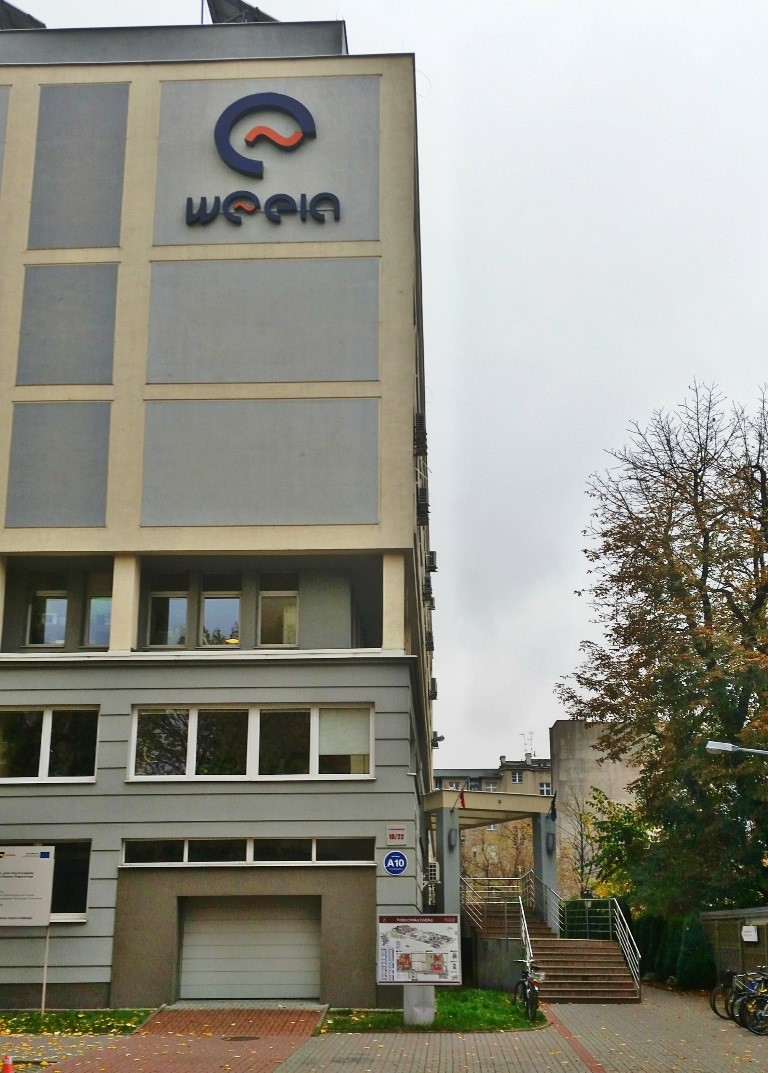
\includegraphics[width=200bp]{The_Headquaters_of_the_Institute_of_Applied_Computer_Science.jpg}
\caption{\href{https://commons.wikimedia.org/wiki/File:The\_Headquaters\_of\_the\_Institute\_of\_Applied\_Computer\_Science.jpg}{The Headquaters of the Institute of Applied Computer Science} - Polônia, CC BY-SA.}\label{\detokenize{AF209-E:id2}}\end{figure}

Sabendo que as medidas estão em metros, determine a altura máxima atingida por esse objeto, uma vez que essa altura foi alcançada a \(2\) metros do prédio.

\needspace{10em}
\item Uma fábrica tem o custo de sua produção descrito no gráfico a seguir.
\begin{figure}[H]
\centering

\begin{tikzpicture}[yscale=.75, every node/.style={scale=2}]

       \draw [->,  thick] (-0.5,0) -- (4,0) node [above left, scale=0.5] {$x$};
       \draw [ ->,  thick] (0,-0.5) -- (0,6) node [below right, scale=0.5] {$y$};
     \draw [ dashed, color=secundario] (0,4.2) -- (1,4.2) -- (1,0);
       \foreach \y in {3,4.2}  \draw  (0.1,\y) -- (-0.1,\y);
       \foreach \x in {1} \draw  (\x,0.1) -- (\x,-0.1);
     \draw [ thick, color=\currentcolor!80,domain=0:2.47] plot (\x,{1.2*\x+3});
       \node [left, scale=0.5] at (0,3) {1500};
       \node [left, scale=0.5] at (0,4.2) {2100};
       \node [below, scale=0.5] at (1,0) {10};
\end{tikzpicture}
\end{figure}

\(x\) representa a quantidade de unidades produzidas e \(y\) o custo total, em reais, para produzir essas quantidades.
Considere que o preço de venda das \(x\) unidades produzidas seja \(220 – x\); Lembre-se que o lucro é a diferença entre o que se arrecada e o gasto que se tem. Nessas condições, qual deve ser a quantidade \(x\) produzida para se obter o lucro máximo?

\item (\textbf{UERJ-2005}) Numa operação de salvamento marítimo, foi lançado um foguete sinalizador que permaneceu aceso durante toda sua trajetória. Considere que a altura \(h\), em metros, alcançada por este foguete, em relação ao nível do mar, é descrita por \(h = 10 + 5t - t^2\), em que \(t\) é o tempo, em segundos, após seu lançamento. A luz emitida pelo foguete é útil apenas a partir de \(14\) m acima do nível do mar. O intervalo de tempo, em segundos, no qual o foguete emite luz útil é igual a:
\begin{enumerate}
\item 3
\item 4
\item 5
\item 6
\end{enumerate}

\item (\textbf{UFRJ}) Considere a função \(y = f(x)\) definida por:
\begin{quote}

\(y = f(x) = \left\{ \begin{array}{rlll} 4x, & \text{se} & 0 \leq x \leq 2 \\ -x^2+6x, & \text{se} & 2 \leq x \leq 6 \\ \end{array} \right.\)
\end{quote}
\begin{enumerate}
\item {} 
Esboce o gráfico de \(y = f(x)\) no intervalo de \([0,6]\);

\item {} 
Para que valores de \(x\) temos \(f(x) = 5\) ?

\end{enumerate}

\clearpage
\item (\textbf{AFA}) O retângulo, com base no eixo das abcissas, está inscrito numa parábola, conforme figura abaixo. O valor de  \(x\)  que faz esse retângulo ter perímetro máximo é
\begin{figure}[H]
\centering

\begin{tikzpicture}
\begin{scope}[every node/.style={scale=10/6}, yscale=.4]
\draw [, fill=terciario!50] (-1.25,0) -- (-1.25,4.875) -- (1.25,4.875) -- (1.25,0) -- cycle;
\draw [ thick, ->] (-3,0) -- (3,0) node [above left, scale=0.6] {$x$};
\draw [ thick, ->] (0,-2) -- (0,10) node [below right, scale=0.6] {$y$};
\draw [ thick, color=\currentcolor!80, domain=-2.1:2.1] plot (\x,{-2*(\x)^2+8});
\node [ponto] at (-2,0) {};
\node [ponto] at (2,0) {};
\node [ponto] at (0,8) {};
\node [above left, scale=0.6] at (0,8) {8};
\node [above left, scale=0.6] at (-2,0) {-2};
\node [above right, scale=0.6] at (2,0) {2};
\node [ponto] at (1.25,4.875) {};
\node [ponto] at (-1.25,4.875) {};
\node [below, scale=0.6] at (1.25,0) {$x$};
\node [below, scale=0.6] at (-1.25,0) {-$x$};
\end{scope}
\end{tikzpicture}
\end{figure}
\begin{enumerate}
\item 1
\item 0,5
\item 0,25
\item 1,25
\end{enumerate}

\item (\textbf{ENEM-2010}) Nos processos industriais, como na indústria de cerâmica, é necessário o uso de fornos capazes de produzir elevadas temperaturas e, em muitas situações, o tempo de elevação dessa temperatura deve ser controlado, para garantir a qualidade do produto final e a economia do processo.
Em uma indústria de cerâmica, o forno é programado para elevar a temperatura ao longo do tempo de acordo
com a função:

\begin{equation*}
T(t) = \left\{ \begin{array}{rlll}\displaystyle \frac{7}{5}t+20, & \text{para} & 0 \leq t < 100 \\\displaystyle \frac{2}{125}t^2- \frac{16}{5}t +320, & \text{para} & t \geq 100 \\ \end{array} \right.
\end{equation*}

em que \(T\) é o valor da temperatura atingida pelo forno, em graus Celsius, e \(t\) é o tempo, em minutos, decorrido desde o instante em que o forno é ligado.
Uma peça deve ser colocada nesse forno quando a temperatura for \(48 \,^{o}C\) e retirada quando a temperatura for \(200 \,^{o}C\).

O tempo de permanência dessa peça no forno é, em
minutos, igual a:
\begin{enumerate}
\item 100
\item 108
\item 128
\item 130
\item 150
\end{enumerate}
\clearpage

\item (\textbf{UERJ - 2010}) Um terreno retangular tem \(800\) m de perímetro e será dividido pelos segmentos \(\overline{PA}\) e \(\overline{CQ}\) em três partes, como mostra a figura.

\begin{figure}[H]
\centering

\begin{tikzpicture}
\begin{scope} [scale=2, every node/.style={scale=2}]
\draw [fill=\currentcolor!80, color=\currentcolor!80] (0,0) -- (2.5,0) -- (2.5,1.5) -- (0,1.5) -- cycle;
\draw [fill=atento, color=secundario!50] (0,0) -- (1.666666,1.5) -- (2.5,1.5) -- (0.833333,0) -- cycle;
\draw [densely dashed, color=secundario] (0,0) -- (1.6666,1.5);
\draw [densely dashed, color=secundario] (0.83333,0) -- (2.5,1.5);
\node [above, scale=0.5] at (0,1.5) {D};
\node [below, scale=0.5] at (0,0) {A};
\node [below, scale=0.5] at (0.833333,0) {Q};
\node [below, scale=0.5] at (2.5,0) {B};
\node [above, scale=0.5] at (1.66666,1.5) {P};
\node [above, scale=0.5] at (2.5,1.5) {C};
\end{scope}
\end{tikzpicture}
\end{figure}

Admita que os segmentos de reta \(\overline{PA}\) e \(\overline{CQ}\) estão contidos nas bissetrizes de dois ângulos retos do terreno e que a área do paralelogramo \(PAQC\) tem medida \(S\).
Determine o maior valor, em \(m^2\) , que \(S\) pode assumir.

\item (\textbf{UERJ - 2012}) Distância de frenagem é aquela percorrida por um carro do instante em que seu freio é acionado até o momento em que ele para. Essa distância é diretamente proporcional ao quadrado da velocidade que o carro está desenvolvendo no instante em que o freio é acionado.

\begin{figure}[H]
\centering

\begin{tikzpicture}
[scale=0.75, every node/.style={scale=2.5}]
\draw [ thick, color=\currentcolor!80, domain=0:7.3] plot (\x,{0.128*(\x)^2});
\draw [ thick, ->] (-0.5,0) -- (7.5,0) node [below right, scale=0.4] {$v$(km/h)};
\draw [ thick, ->] (0,-0.5) -- (0,7) node [below left, scale=0.4] {$d$(m)};
\draw [dashed] (0,3.2) -- (5,3.2) -- (5,0);
\node[ponto] at (5,3.2){};
\node [below, scale=0.4] at (5,0) {50};
\node [below left, scale=0.4] at (0,0) {0};
\node [left, scale=0.4] at (0,3.2) {32};
\end{tikzpicture}
\end{figure}

O gráfico abaixo indica a distância de frenagem \(d\), em metros, percorrida por um carro, em função de sua velocidade \(v\), em quilômetros por hora.

Admita que o freio desse carro seja acionado quando ele alcançar a velocidade de \(100\) km/h.

Calcule sua distância de frenagem, em metros.


\clearpage
\item (\textbf{ENEM - 2013}) A parte interior de uma taça foi gerada pela rotação de uma parábola em torno de um eixo \(z\), conforme mostra a figura.

\begin{figure}[H]
\centering

\begin{tikzpicture}
[yscale=0.333333, every node/.style={scale=3.3333}, scale=.75]
       \draw [ , ->] (-1,0) -- (6,0) node [below left, scale=0.3] {$x$ (cm)};
       \draw [ , ->,] (0,-8) -- (0,12) node [below left,scale=0.3] {$y$ (cm)};
       \draw  [domain=0:4, fill=destacado!70!black] plot (\x,{3/2*(\x)^2-6*\x+6});
       \draw [thin, fill=destacado!70!black] (2,6) ellipse (2cm and 1cm);
       \draw [ ] (2,9.375) ellipse (2.5cm and 1.5cm);
     \draw [ , domain=-0.5:4.5] plot (\x,{3/2*(\x)^2-6*\x+6});
       \draw [ ] (2,-6) ellipse (1cm and 0.8cm);
       \draw [,fill=white] (2,-6) ellipse (0.2 cm and 0.2cm);
       \draw [ , fill=white] (1.8,0) rectangle (2.2,-6);
       \draw [white,  ] (1.82,-6) -- (2.18,-6);
       \draw [dashed, ->, color=secundario] (2,6) -- (2,12) node [right, color=black, scale=0.3] {$z$ Eixo de rotacao};
       \node [ponto] at (0,6) {} node at (0,6) [left, scale=0.3] {$C$} node [ponto] at (2,0) {} node [below, scale=0.3] at (2,0) {$V$};
\end{tikzpicture}
\end{figure}

A função real que expressa a parábola, no plano cartesiano da figura, é dada pela lei \(\displaystyle f(x)=\frac{3}{2}x^2-6x+C\), onde \(C\) é a medida da altura do líquido contido na taça, em centímetros. Sabe-se que o ponto \(V\), na figura, representa o vértice da parábola, localizado sobre o eixo \(x\).
Nessas condições, a altura do líquido contido na taça, em centímetros, é
\begin{enumerate}
\item 1
\item 2
\item 4
\item 5
\item 6
\end{enumerate}

\needspace{10em}
\item (\textbf{FGV - 2014}) A figura a seguir mostra uma parte do gráfico da função quadrática que simula a trajetória de uma bala de canhão. Com os eixos e escala adequados, o canhão estava no solo, no ponto \((0,0)\) e a bala passou, em seguida, pelos pontos \((1,1)\) e \((4,3)\).
\begin{center}\begin{tikzpicture}[scale=.9,every node/.style={scale=2}]
\draw [dashed,, color=secundario] (0,1) -- (1,1) -- (1,0);
\draw [dashed, , color=secundario] (0,3) -- (4,3) -- (4,0);
\draw [ thick, color=\currentcolor!80, domain=0:4.2] plot (\x,{(-1/12)*(\x)^2+(13/12)*\x});
\draw [ thick, ->] (-0.5,0) -- (4.5,0) node [below, scale=0.6] {$x$};
\draw [ thick, ->] (0,-0.5) -- (0,3.5) node [left, scale=0.6] {$y$};
\foreach \x in {1,...,4} \node [below, scale=0.5] at (\x,0) {\x};
\foreach \y in {1,...,3} \node [left, scale=0.5] at (0,\y) {\y};
\foreach \x in {1,...,4} \draw [] (\x,0.05) -- (\x,-0.05);
\foreach \y in {1,...,3} \draw [] (0.05,\y) -- (-0.05,\y);
\draw [dashed] (0,1) -- (1,1) -- (1,0);
\draw [dashed] (0,3) -- (4,3) -- (4,0);
\node [ponto,color=secundario] at (1,1) {};
\node [ponto, color=secundario] at (4,3) {};
\node [below left, scale=0.5] at (0,0) {0};
\end{tikzpicture}\end{center}
A bala atingirá o solo no ponto
\begin{enumerate}
\item (11,0)
\item (14,0)
\item (13,0)
\item (12,0)
\item (15,0)
\end{enumerate}

\item (\textbf{FUVEST}) A trajetória de um projétil, lançado da beira de um penhasco sobre um terreno plano e horizontal, é parte de uma parábola com eixo de simetria vertical, como ilustrado na figura. O ponto \(P\) sobre o terreno, pé da perpendicular traçada a partir do ponto ocupado pelo projétil, percorre \(30m\) desde o instante do lançamento até o instante em que o projétil atinge o solo. A altura máxima do projétil, de \(200m\) acima do terreno, é atingida no instante
em que a distância percorrida por \(P\), a partir do instante do lançamento, é de \(10m\). Quantos metros acima do terreno estava o projétil quando foi lançado?

\begin{figure}[H]
\centering
\capstart

\noindent\includegraphics[width=150bp]{{Vertical_granite_cliff_at_sunset}.jpg}
\caption{Foto de \href{https://commons.wikimedia.org/wiki/File:Vertical\_granite\_cliff\_at\_sunset.jpg}{W. Carter} CC-BY.}\label{\detokenize{AF209-E:id3}}\end{figure}
\begin{enumerate}
\item 60
\item 90
\item 120
\item 150
\item 180
\end{enumerate}

\item (\textbf{ITA}) Os dados experimentais da tabela a seguir correspondem às concentrações de uma substância química medida em intervalos de \(1\) segundo.

\begin{table}[H]
\centering
\begin{tabu} to \textwidth{|c|c|c}
\hline
\thead
Tempo (s) & Concentração (moles) \\
\hline
\(1\) & \(3\text{,}00\) \\
\hline
\(2\) & \(5\text{,}00\) \\
\hline
\(3\) & \(1\text{,}00\) \\
\hline
\end{tabu}
\end{table}

Assumindo que a linha que passa pelos três pontos experimentais é uma parábola, tem-se que a concentração (em moles) após \(2\text{,}5\) segundos é:
\begin{enumerate}
\item 3,60
\item 3,65
\item 3,70
\item 3,75
\item 3,80
\end{enumerate}

\item Uma ponte será sustentada por dois cabos principais,  cujo formato consideraremos o de um arco parabólico. A ponte terá \(60\) m de comprimento e, a cada \(10\) m, haverá um apoio vertical, ligando a ponte com o cabo principal, estabilizando a estrutura. A figura abaixo exibe o esquema de um dos lados dessa ponte.
\begin{center}\begin{tikzpicture}
[every node/.style={scale=2.5}]
       \draw [very thick, fill=secundario!70] (-0.5,-1.5) rectangle (0,2);
       \draw [very thick, fill=secundario!70] (6,-1.5) rectangle (6.5,2);
       \draw [very thick] (0,0) -- (6,0);
       \draw [very thick](1,0) -- (1,0.905);
       \draw [very thick](5,0) -- (5,0.905);
       \draw [very thick] (2,0) -- (2,0.2);
     \draw [very thick] (4,0) -- (4,0.2);
       \draw (-0.8,0) -- (-0.8,2);
       \node [left,scale=0.4] at (-0.8,1) {20m};
       \node [left,scale=0.4] at (6.8,1) {\phantom{20m}};
       \foreach\x in {1,...,5} \node [below,scale=0.4] at (\x,0) {\x0};
       \node  [scale=0.4] [below right] at (0,0) {0};
     \node [below left, scale=0.4] at (6,0) {60};
       \draw [very thick, domain=0:6] plot (\x,{(1/4.5)*((\x)^2)-4/3*(\x)+2});
\end{tikzpicture}\end{center}
O valor do metro do apoio vertical é R\$ \(500\text{,}00\). Nessas condições, calcule o gasto com os apoios verticais para a construção dessa ponte. (Use a aproximação \(\frac{10}{9} = 1\)).

\item Uma pizzaria só vende pizza de tamanho individual. Ela cobra R\$ \(15\text{,}00\) por cada pizza e considera como um padrão a venda de \(80\) pizzas por dia.

\begin{figure}[H]
\centering
\capstart

\noindent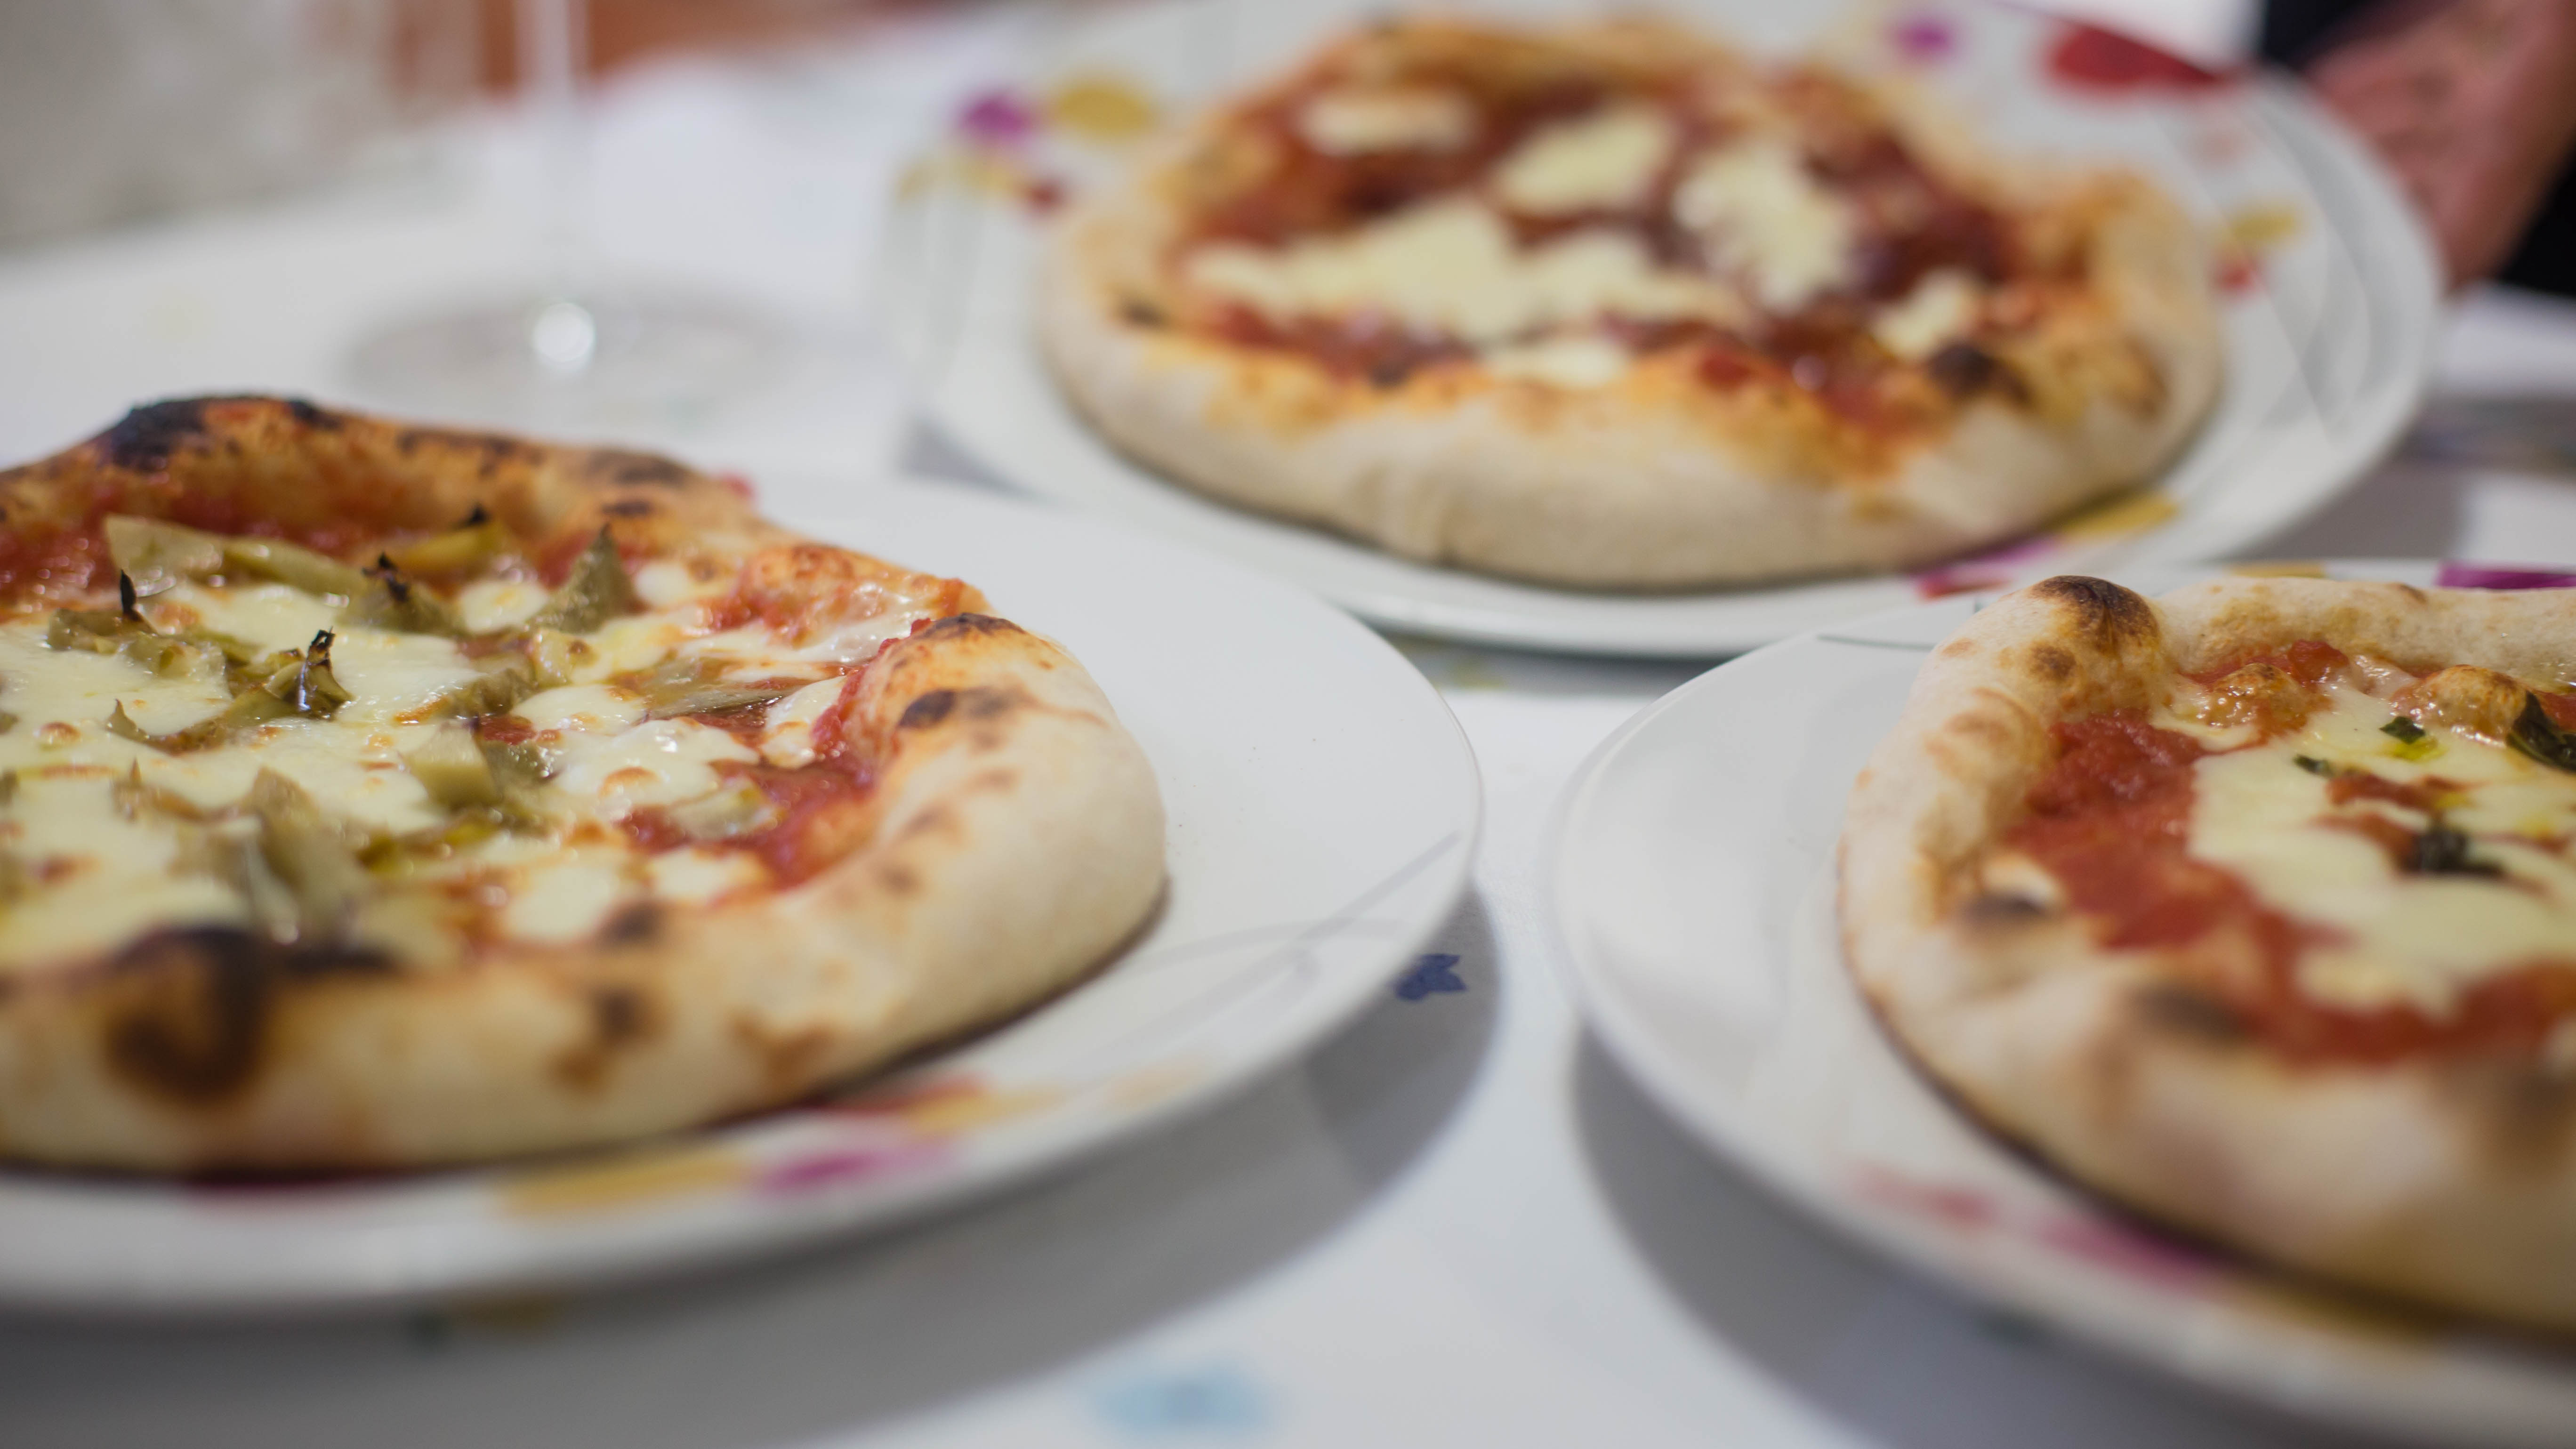
\includegraphics[width=200bp]{Pizza_(17425076966).jpg}
\caption{Foto do \href{https://commons.wikimedia.org/wiki/File:Pizza\_(17425076966).jpg}{Nicola} CC BY.}\label{\detokenize{AF209-E:id4}}\end{figure}
\needspace{5em}
Um estudo foi contratato e realizado na vizinhaça dessa pizzaria, em lojas, escolas, escritórios e pontos de ônibus. A conclusão revelou que a cada real reduzido no preço da pizza, aumentaria em 10 a quantidade padrão de venda de pizzas por dia. Nessas condições, responda:
\begin{enumerate}
\item {} 
Quanto arrecada em um dia essa pizzaria, cobrando R\$ \(15\text{,}00\) por pizza?

\item {} 
Quanto arrecada em um dia essa pizzaria, cobrando R\$ \(10\text{,}00\) por pizza?

\item {} 
Qual é o valor ideal para o preço da pizza deste estabelecimento, de modo a tornar máxima a arrecadação?

\item {} 
Com o valor ideal, qual o ganho diário esperado?

\end{enumerate}
\end{enumerate}

\ifnum\aluno=1
\clearpage
\else
\notasfinais
\fi

\bibliographystyle{apalike-pt}
\bibliography{../Bibliografia/funcao-quadratica_bibliografia.bib}

\nocite{*}